\documentclass{article}
\usepackage{titling}
\newcommand{\subtitle}[1]{\posttitle{\par\end{center}\begin{center}\large#1\end{center}\vskip0.5em}}
\usepackage[left=1.5cm, right=1.5cm, top=1.5cm, bottom=1.5cm]{geometry}
\usepackage{graphicx, float}
\usepackage[font=footnotesize,labelfont=bf,belowskip=0pt,aboveskip=2pt]{caption}
\usepackage[hidelinks]{hyperref}
\usepackage{fixltx2e}
\usepackage{amsmath,amssymb,mathrsfs}
\usepackage{sidecap}
\usepackage{gensymb}
\setlength\parindent{0pt}
\renewcommand{\floatpagefraction}{.8}
\pagenumbering{gobble}
\usepackage[labelsep=period]{caption}
\usepackage[skip=8pt]{caption}
\renewcommand{\figurename}{}
\renewcommand{\thefigure}{\small{Figure~S\arabic{figure}}}
\sidecaptionvpos{figure}{t}
\usepackage{fontspec}
\setmainfont{Calibri}
\usepackage{atbegshi}
\begin{document}

\renewcommand{\figurename}{\small{Figure}}

%\renewcommand{\thefigure}{S1}
%\begin{figure}[H]
%\centering
%\makebox[\textwidth][c]{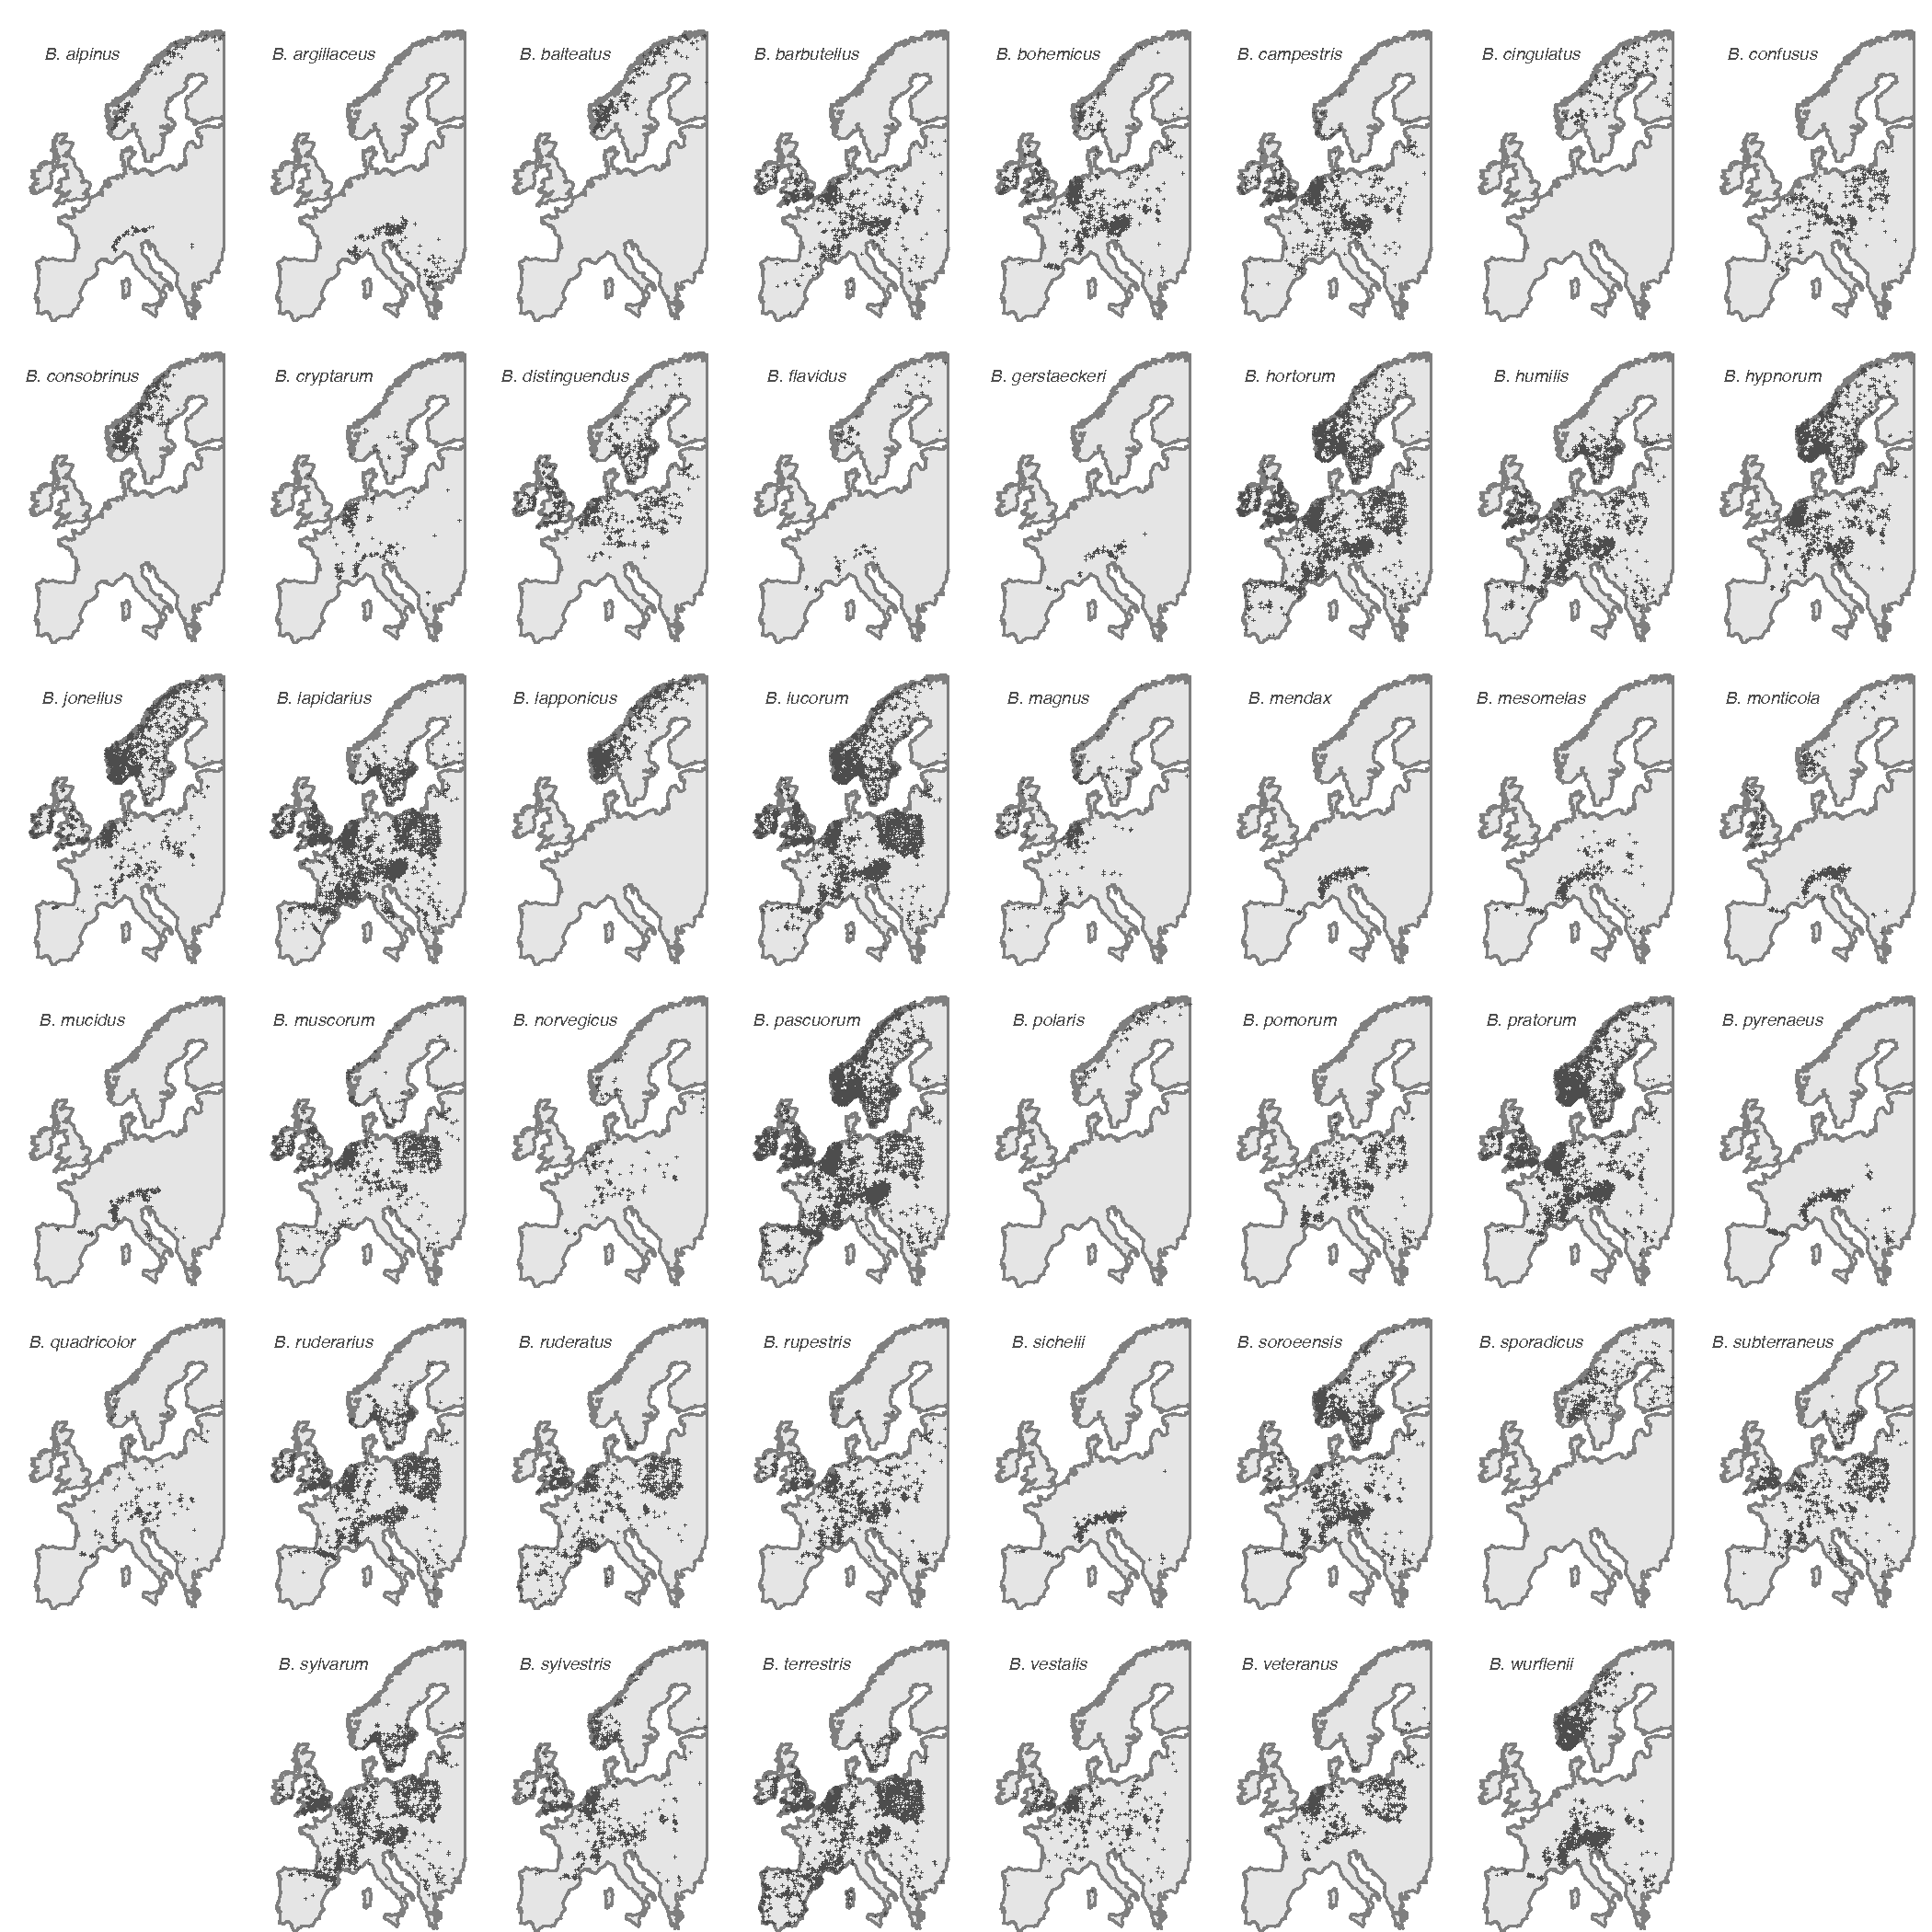
\includegraphics[width=1.00\textwidth]{Bombus_observations_1.pdf}}
%\caption{\small{\textbf{Occurrence data of the European bumblebee species for the first time period (1901-1974).}
%}}
%\label{FigureS1}
%\end{figure}
%
%\renewcommand{\thefigure}{S2}
%\begin{figure}[H]
%\centering
%\makebox[\textwidth][c]{\includegraphics[width=1.00\textwidth]{Bombus_observations_2.pdf}}
%\caption{\small{\textbf{Occurrence data of the European bumblebee species for the second time period (2000-2014).}
%}}
%\label{FigureS2}
%\end{figure}

%\renewcommand{\thefigure}{S3}
%\begin{figure}[H]
%\centering
%\makebox[\textwidth][c]{\includegraphics[width=1.00\textwidth]{Bombus_projections_1.pdf}}
%\caption{\small{\textbf{Ecological niche modelling for the first time period (1901-1974).}
%}}
%\label{FigureS3}
%\end{figure}
%
%\renewcommand{\thefigure}{S4}
%\begin{figure}[H]
%\centering
%\makebox[\textwidth][c]{\includegraphics[width=1.00\textwidth]{Bombus_projections_2.pdf}}
%\caption{\small{\textbf{Ecological niche modelling for the second time period (2000-2014).}
%}}
%\label{FigureS4}
%\end{figure}

\renewcommand{\thefigure}{S1}
\begin{figure}[H]
\centering
\makebox[\textwidth][c]{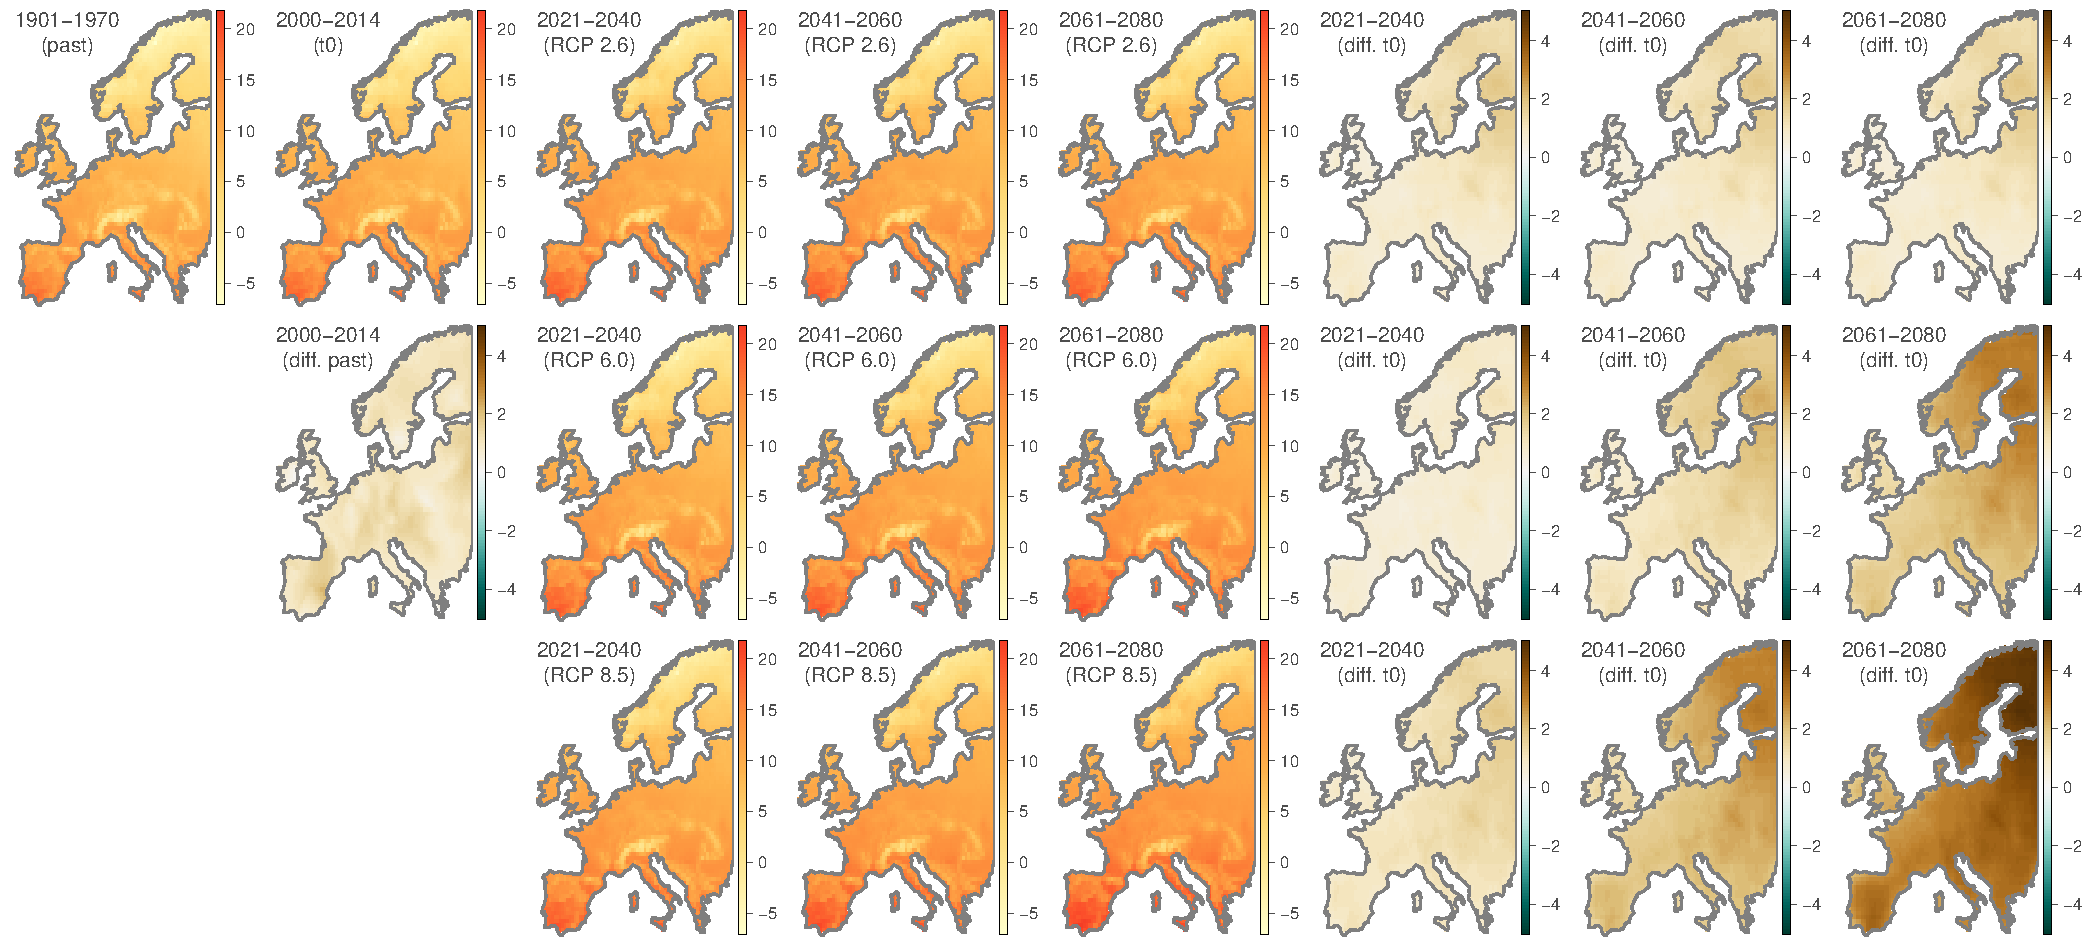
\includegraphics[width=1.00\textwidth]{Environmental_variable_1.pdf}}
\caption{\small{\textbf{1� environmental variable involved in ecological niche modelling: air temperature near surface (�C).}
We here also report the difference between each future estimate and the estimate for the current period (t0).}}
\label{FigureS1}
\end{figure}

\renewcommand{\thefigure}{S2}
\begin{figure}[H]
\centering
\makebox[\textwidth][c]{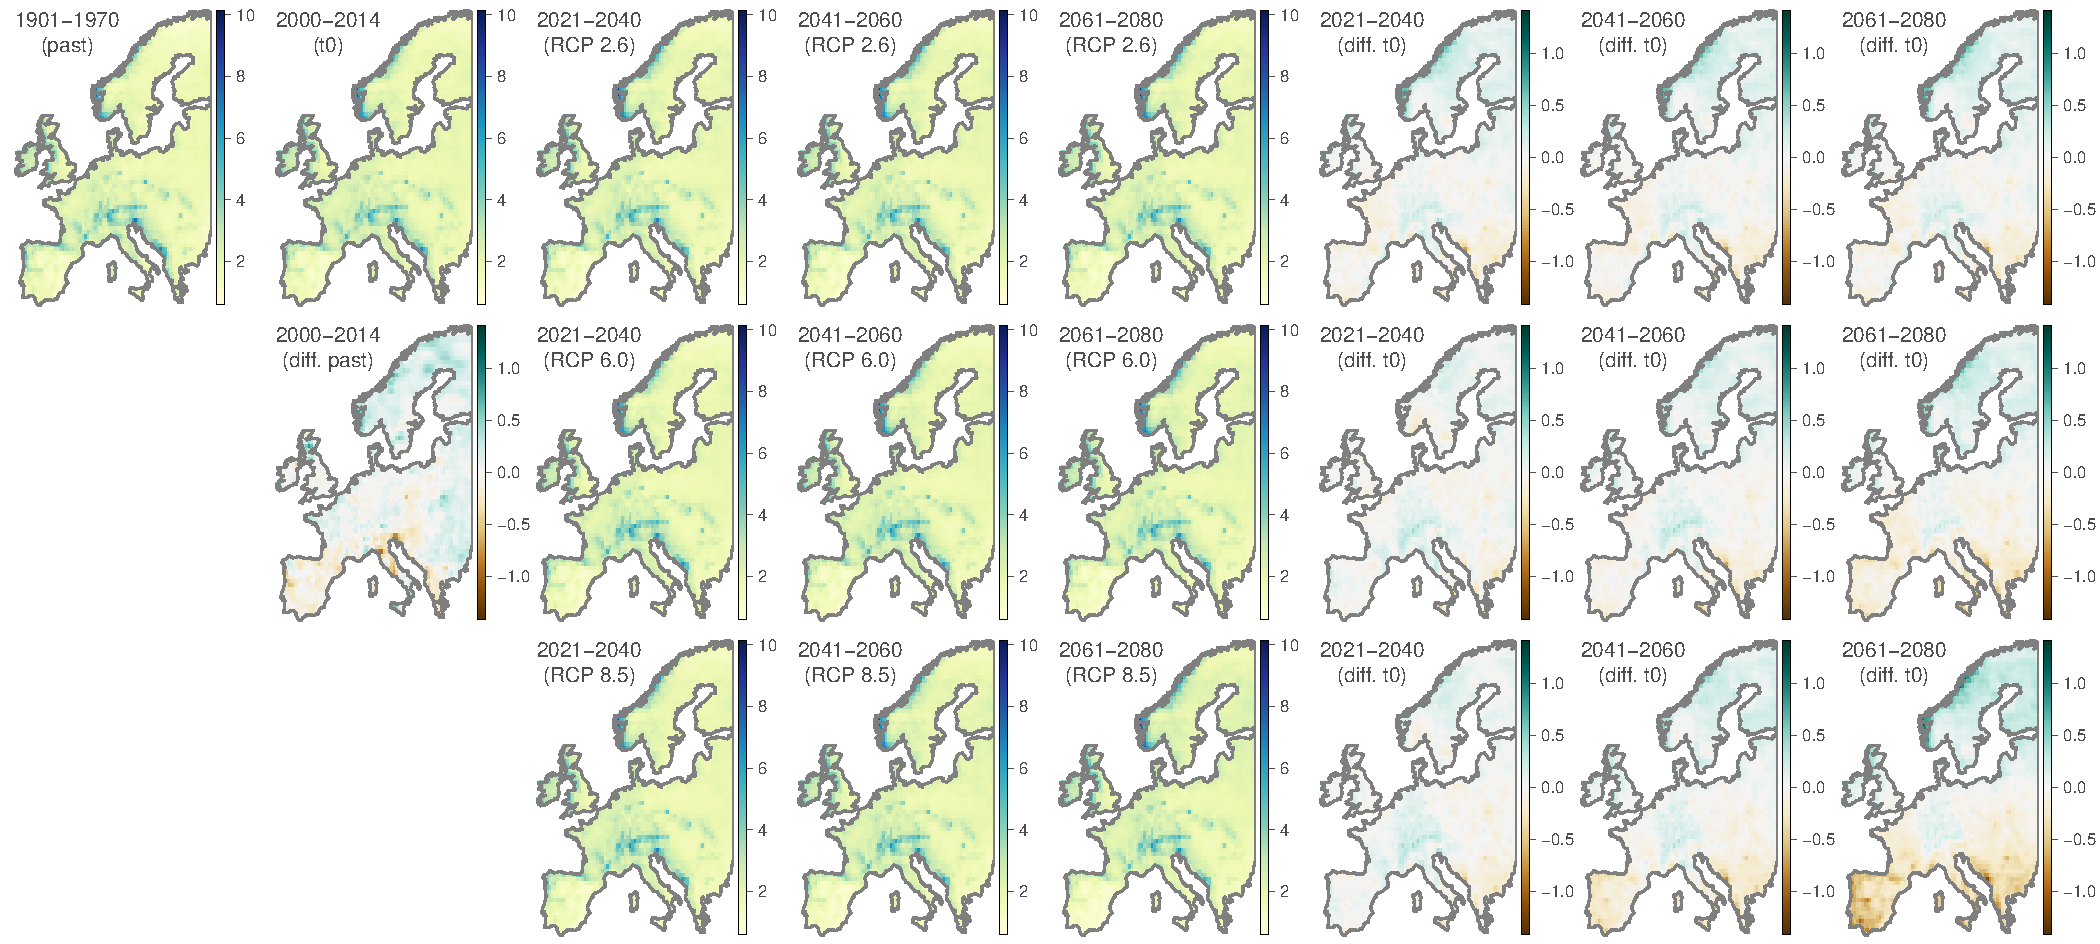
\includegraphics[width=1.00\textwidth]{Environmental_variable_2.pdf}}
\caption{\small{\textbf{2� environmental variable involved in ecological niche modelling: precipitation (kg/m\textsuperscript{2}/day).}
We here also report the difference between each future estimate and the estimate for the current period (t0).}}
\label{FigureS2}
\end{figure}

\renewcommand{\thefigure}{S3}
\begin{figure}[H]
\centering
\makebox[\textwidth][c]{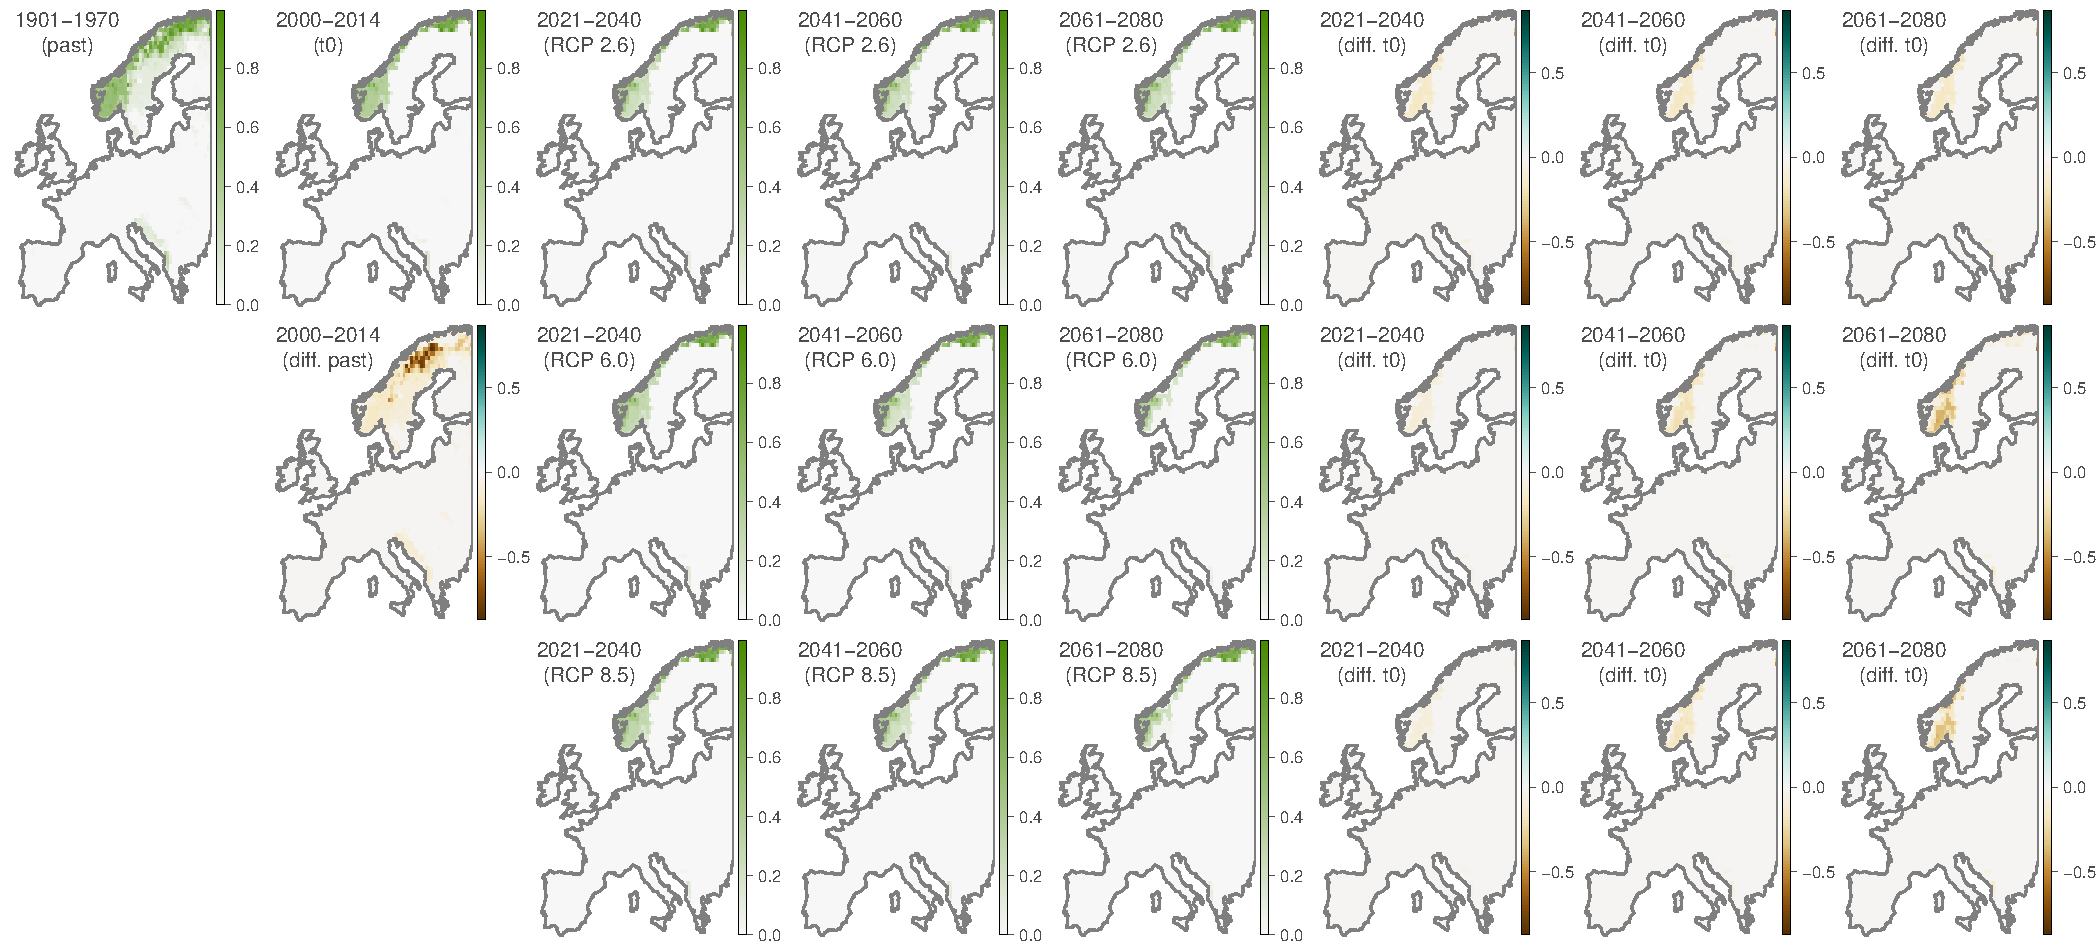
\includegraphics[width=1.00\textwidth]{Environmental_variable_3.pdf}}
\caption{\small{\textbf{3� environmental variable involved in ecological niche modelling: forested primary land.}
We here also report the difference between each future estimate and the estimate for the current period (t0).}}
\label{FigureS3}
\end{figure}

\renewcommand{\thefigure}{S4}
\begin{figure}[H]
\centering
\makebox[\textwidth][c]{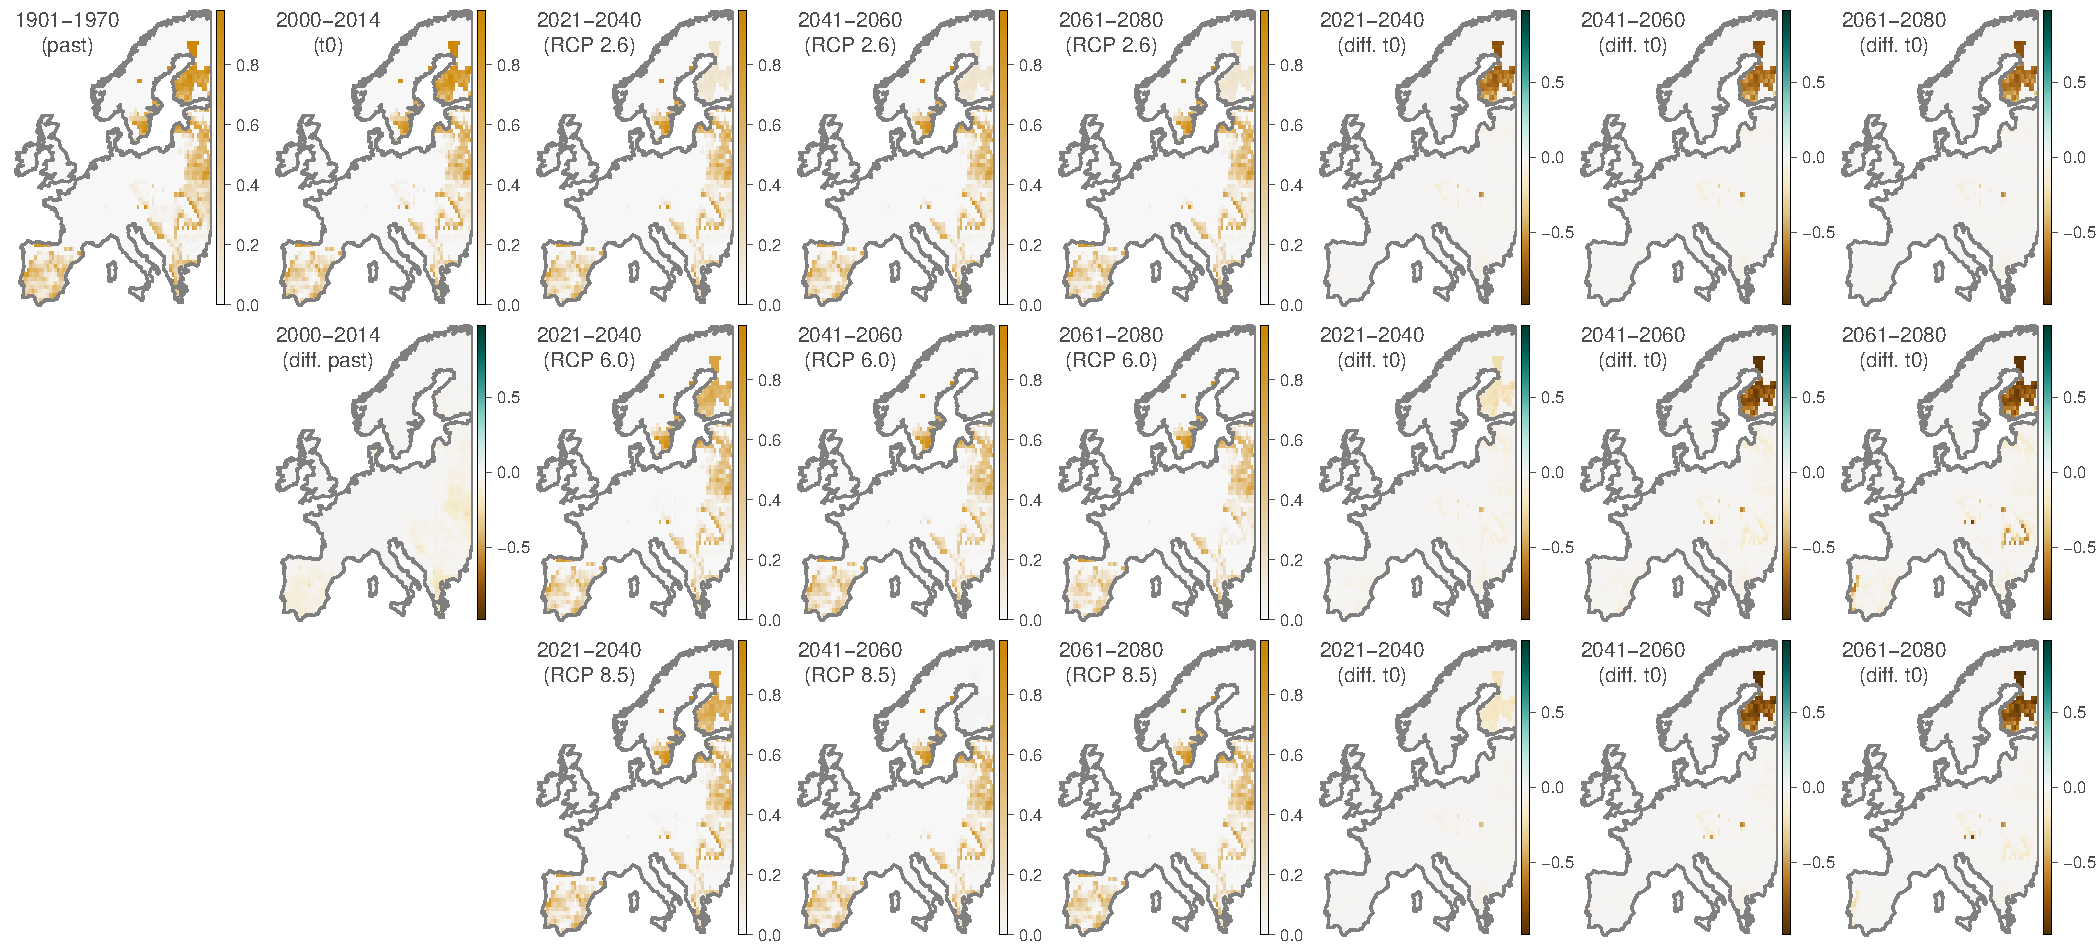
\includegraphics[width=1.00\textwidth]{Environmental_variable_4.pdf}}
\caption{\small{\textbf{4� environmental variable involved in ecological niche modelling: non-forested primary land.}
We here also report the difference between each future estimate and the estimate for the current period (t0).}}
\label{FigureS4}
\end{figure}

\renewcommand{\thefigure}{S5}
\begin{figure}[H]
\centering
\makebox[\textwidth][c]{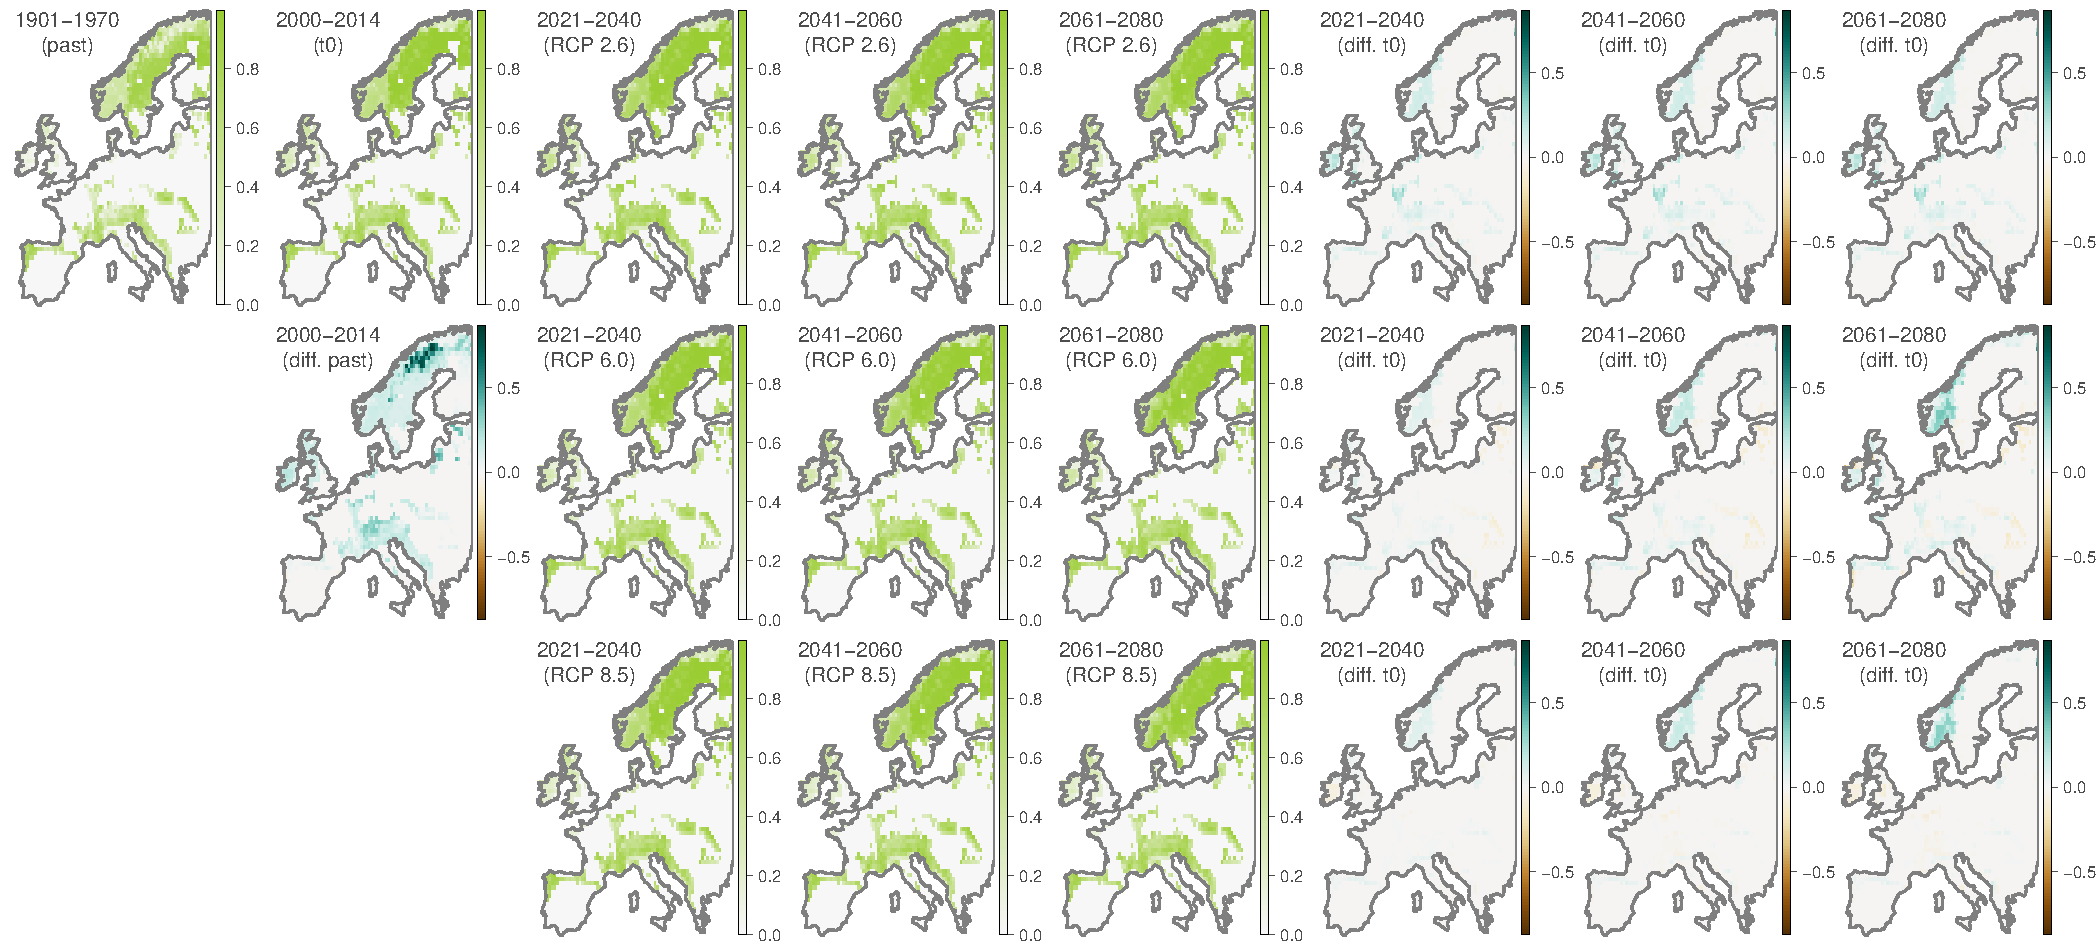
\includegraphics[width=1.00\textwidth]{Environmental_variable_5.pdf}}
\caption{\small{\textbf{5� environmental variable involved in ecological niche modelling: forested secondary land.}
We here also report the difference between each future estimate and the estimate for the current period (t0).}}
\label{FigureS5}
\end{figure}

\renewcommand{\thefigure}{S6}
\begin{figure}[H]
\centering
\makebox[\textwidth][c]{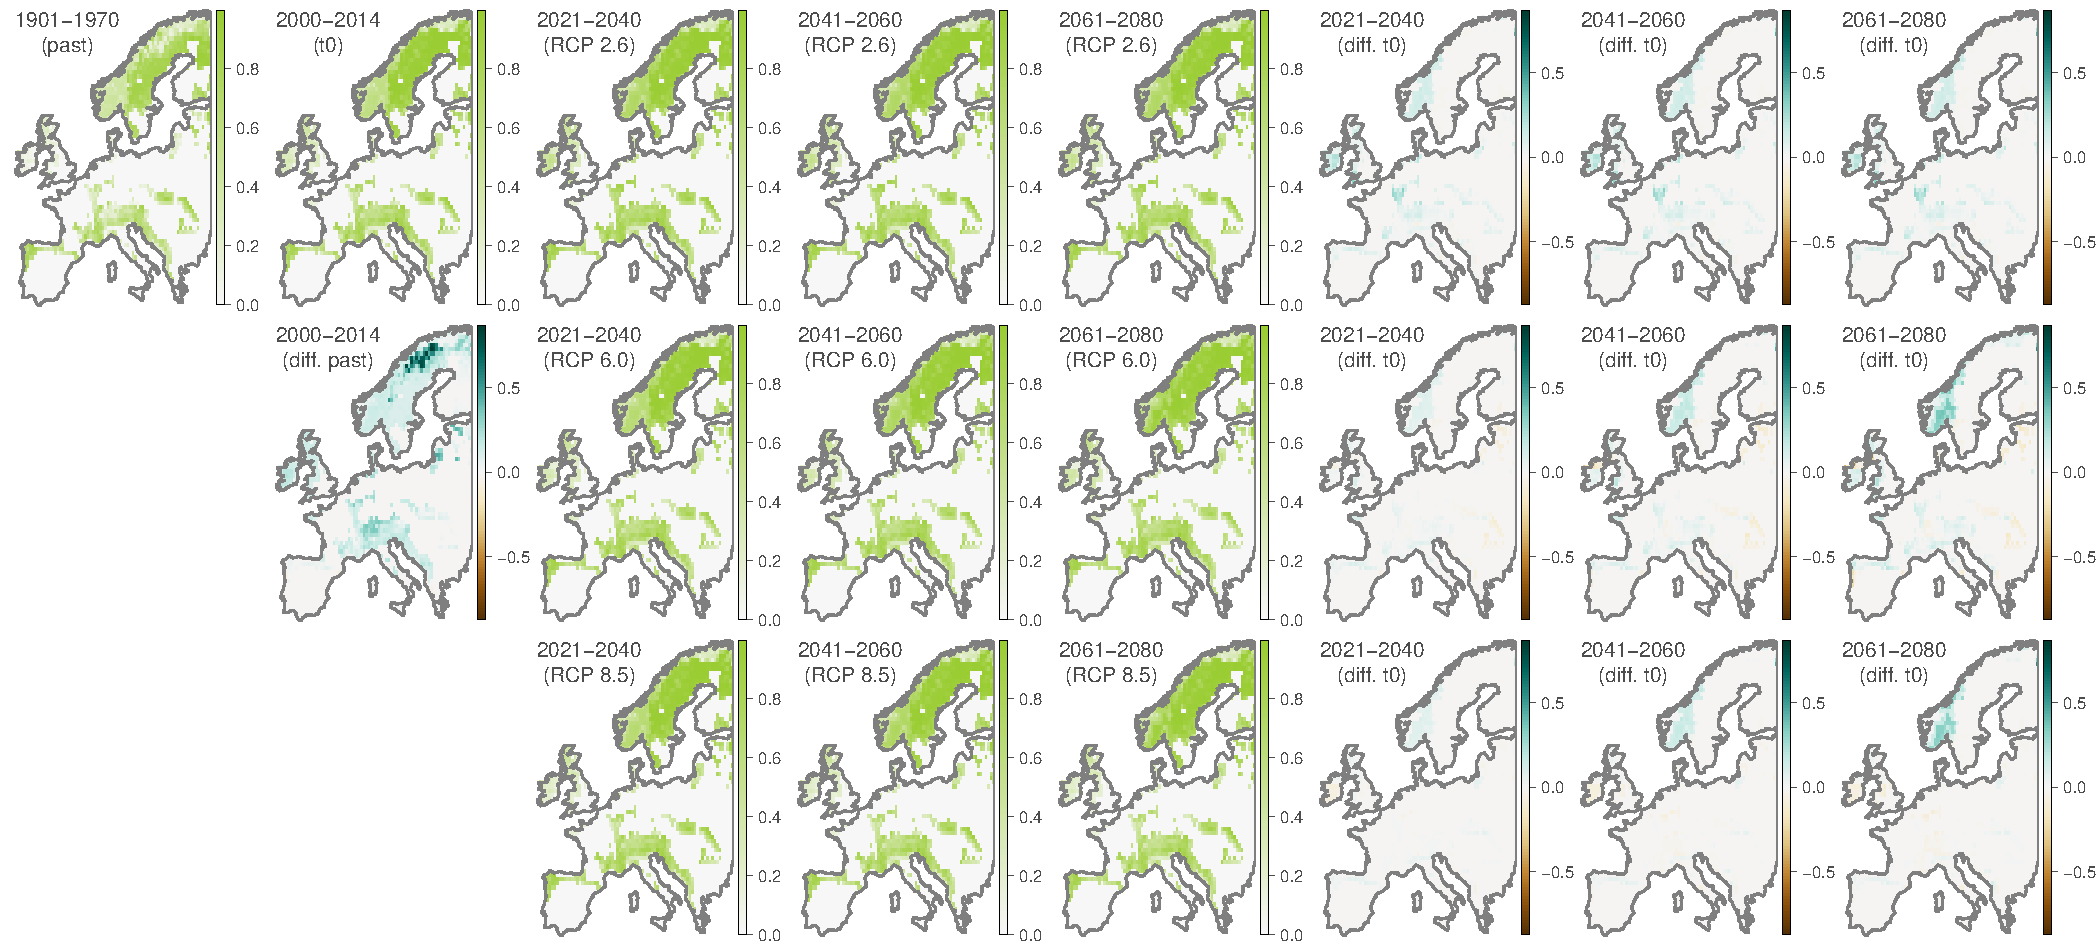
\includegraphics[width=1.00\textwidth]{Environmental_variable_5.pdf}}
\caption{\small{\textbf{6� environmental variable involved in ecological niche modelling: non-forested secondary land.}
We here also report the difference between each future estimate and the estimate for the current period (t0).}}
\label{FigureS6}
\end{figure}

\renewcommand{\thefigure}{S7}
\begin{figure}[H]
\centering
\makebox[\textwidth][c]{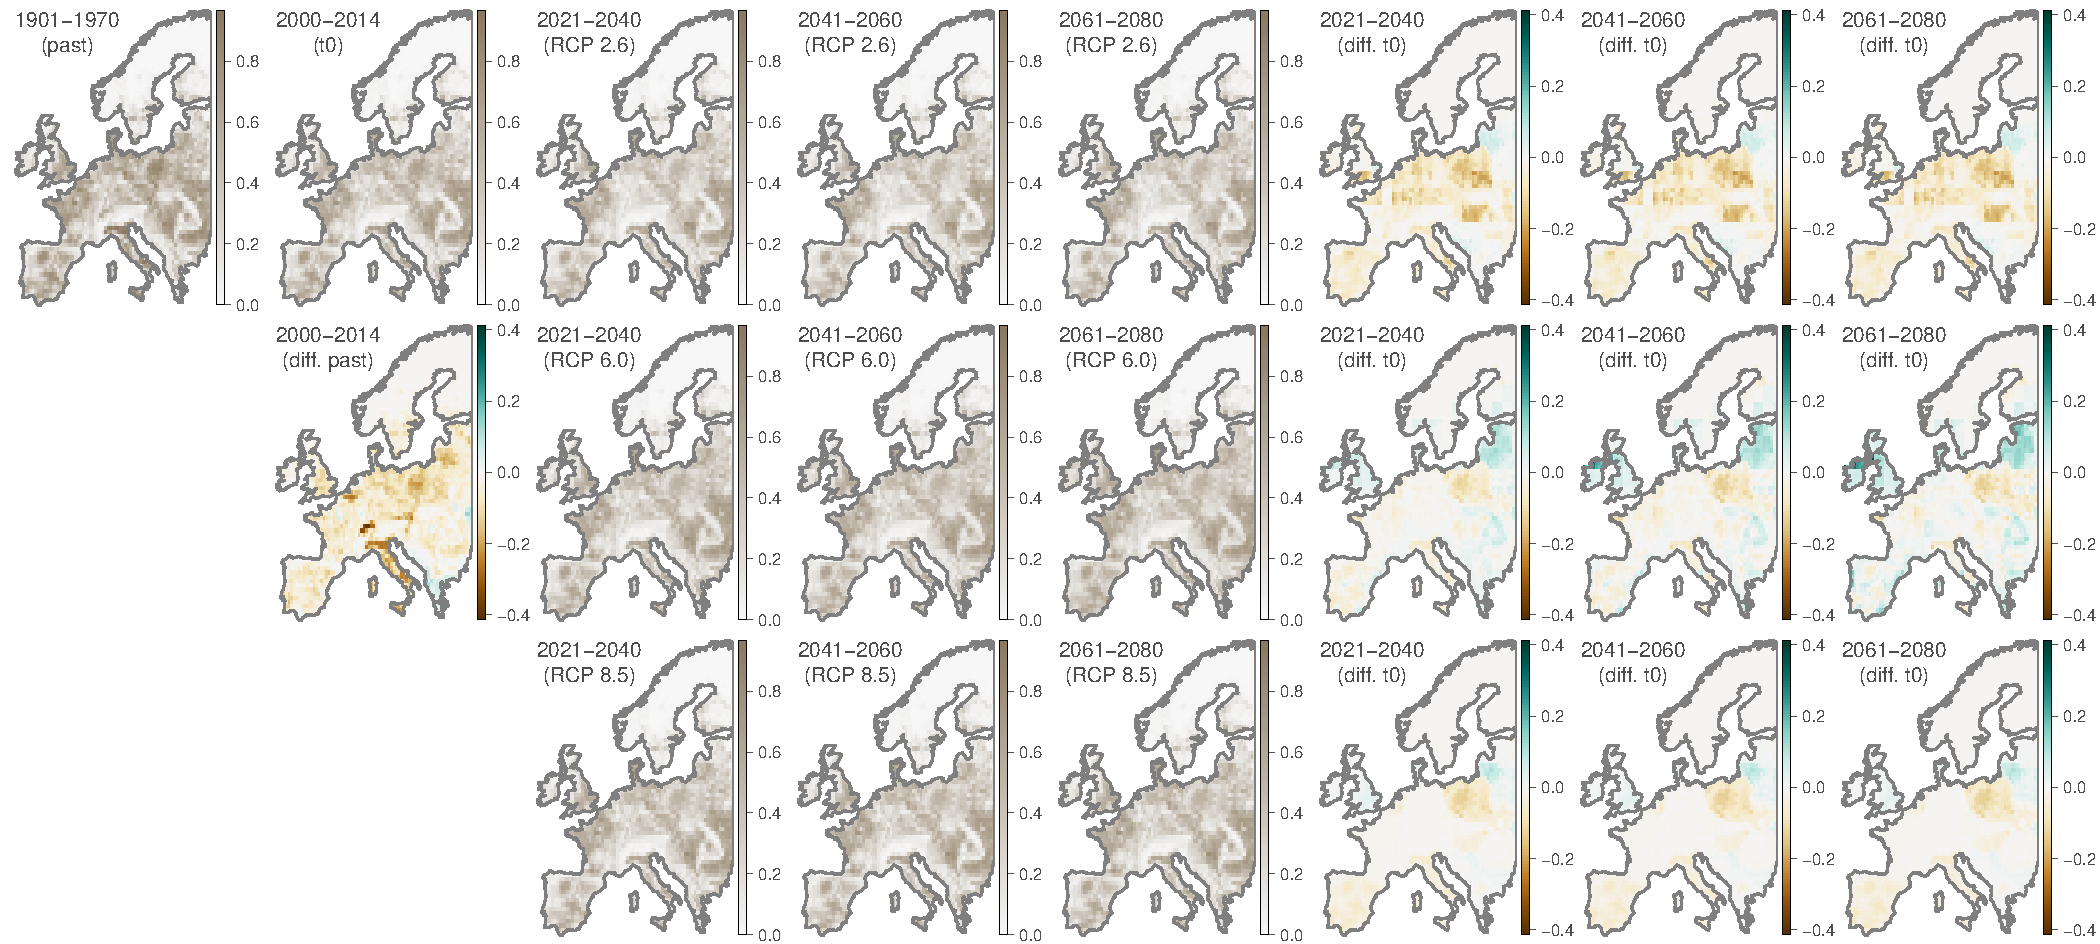
\includegraphics[width=1.00\textwidth]{Environmental_variable_7.pdf}}
\caption{\small{\textbf{7� environmental variable involved in ecological niche modelling: croplands (all categories).}
We here also report the difference between each future estimate and the estimate for the current period (t0).}}
\label{FigureS7}
\end{figure}

\renewcommand{\thefigure}{S8}
\begin{figure}[H]
\centering
\makebox[\textwidth][c]{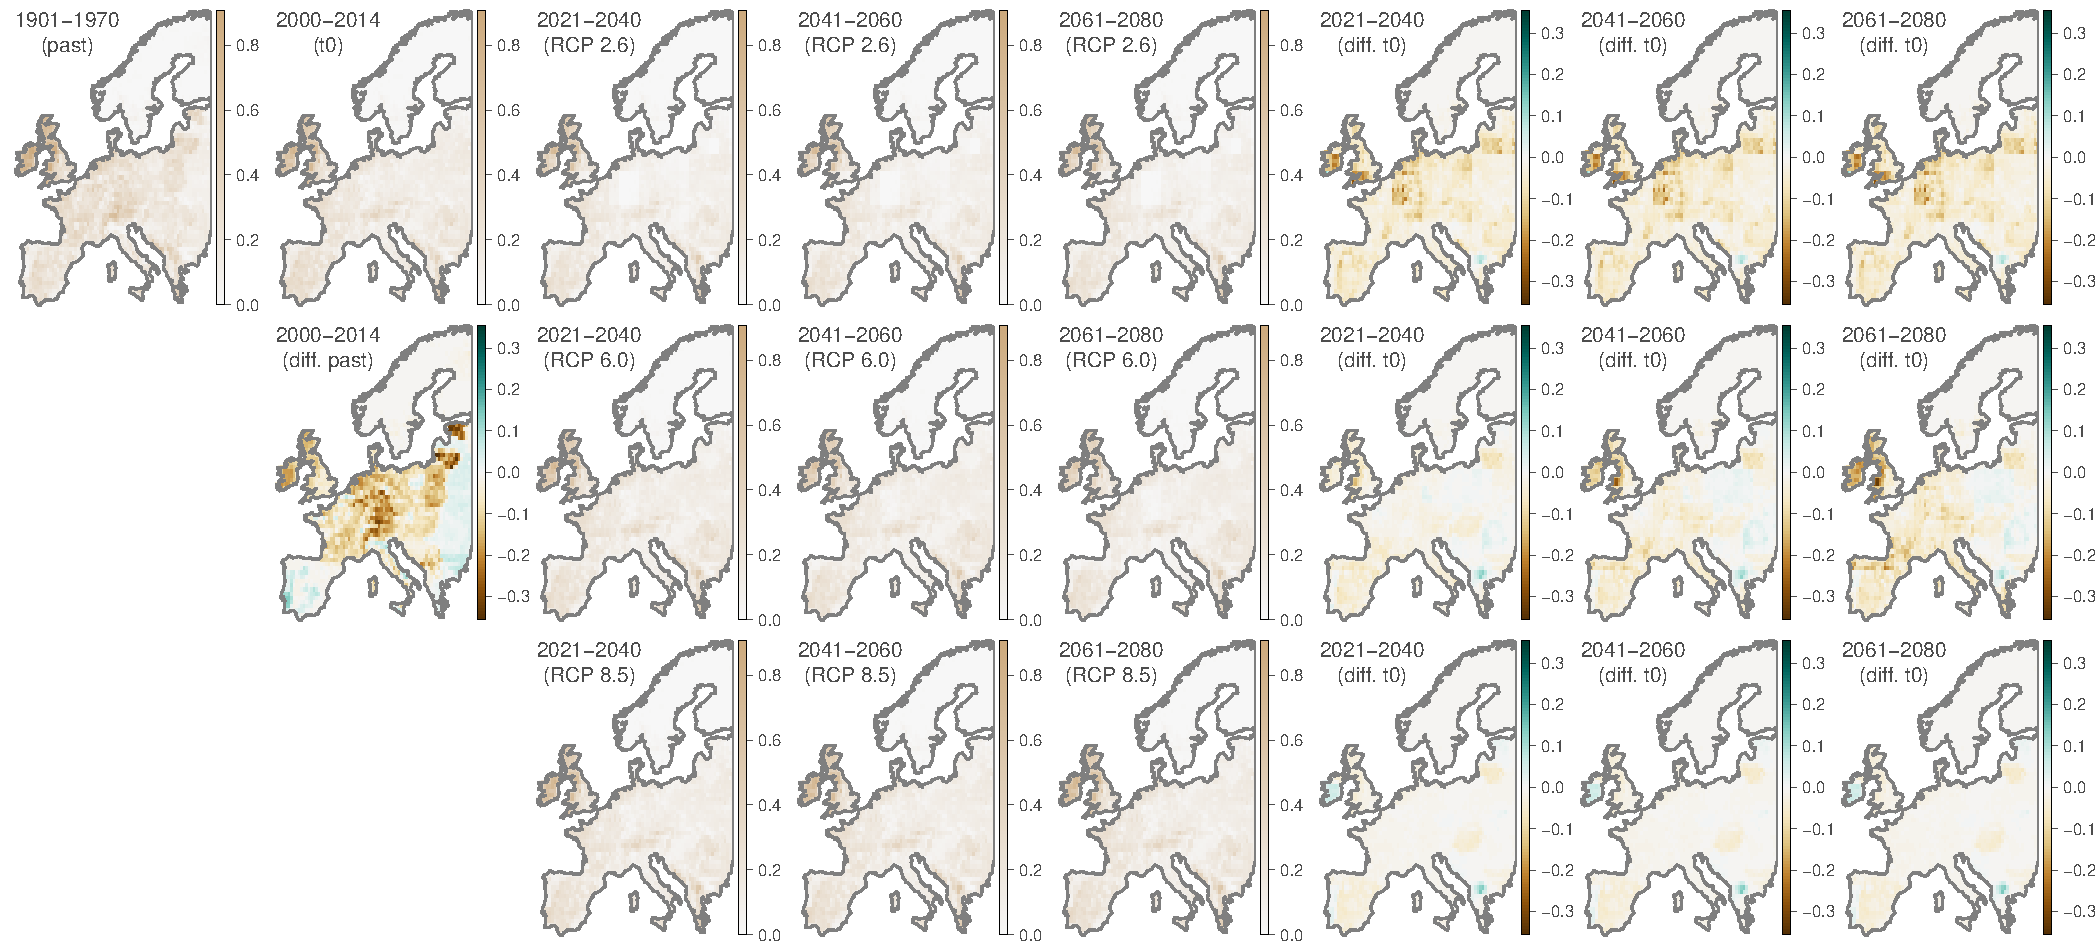
\includegraphics[width=1.00\textwidth]{Environmental_variable_8.pdf}}
\caption{\small{\textbf{8� environmental variable involved in ecological niche modelling: pastures and rangeland.}
We here also report the difference between each future estimate and the estimate for the current period (t0).}}
\label{FigureS8}
\end{figure}

\renewcommand{\thefigure}{S9}
\begin{figure}[H]
\centering
\makebox[\textwidth][c]{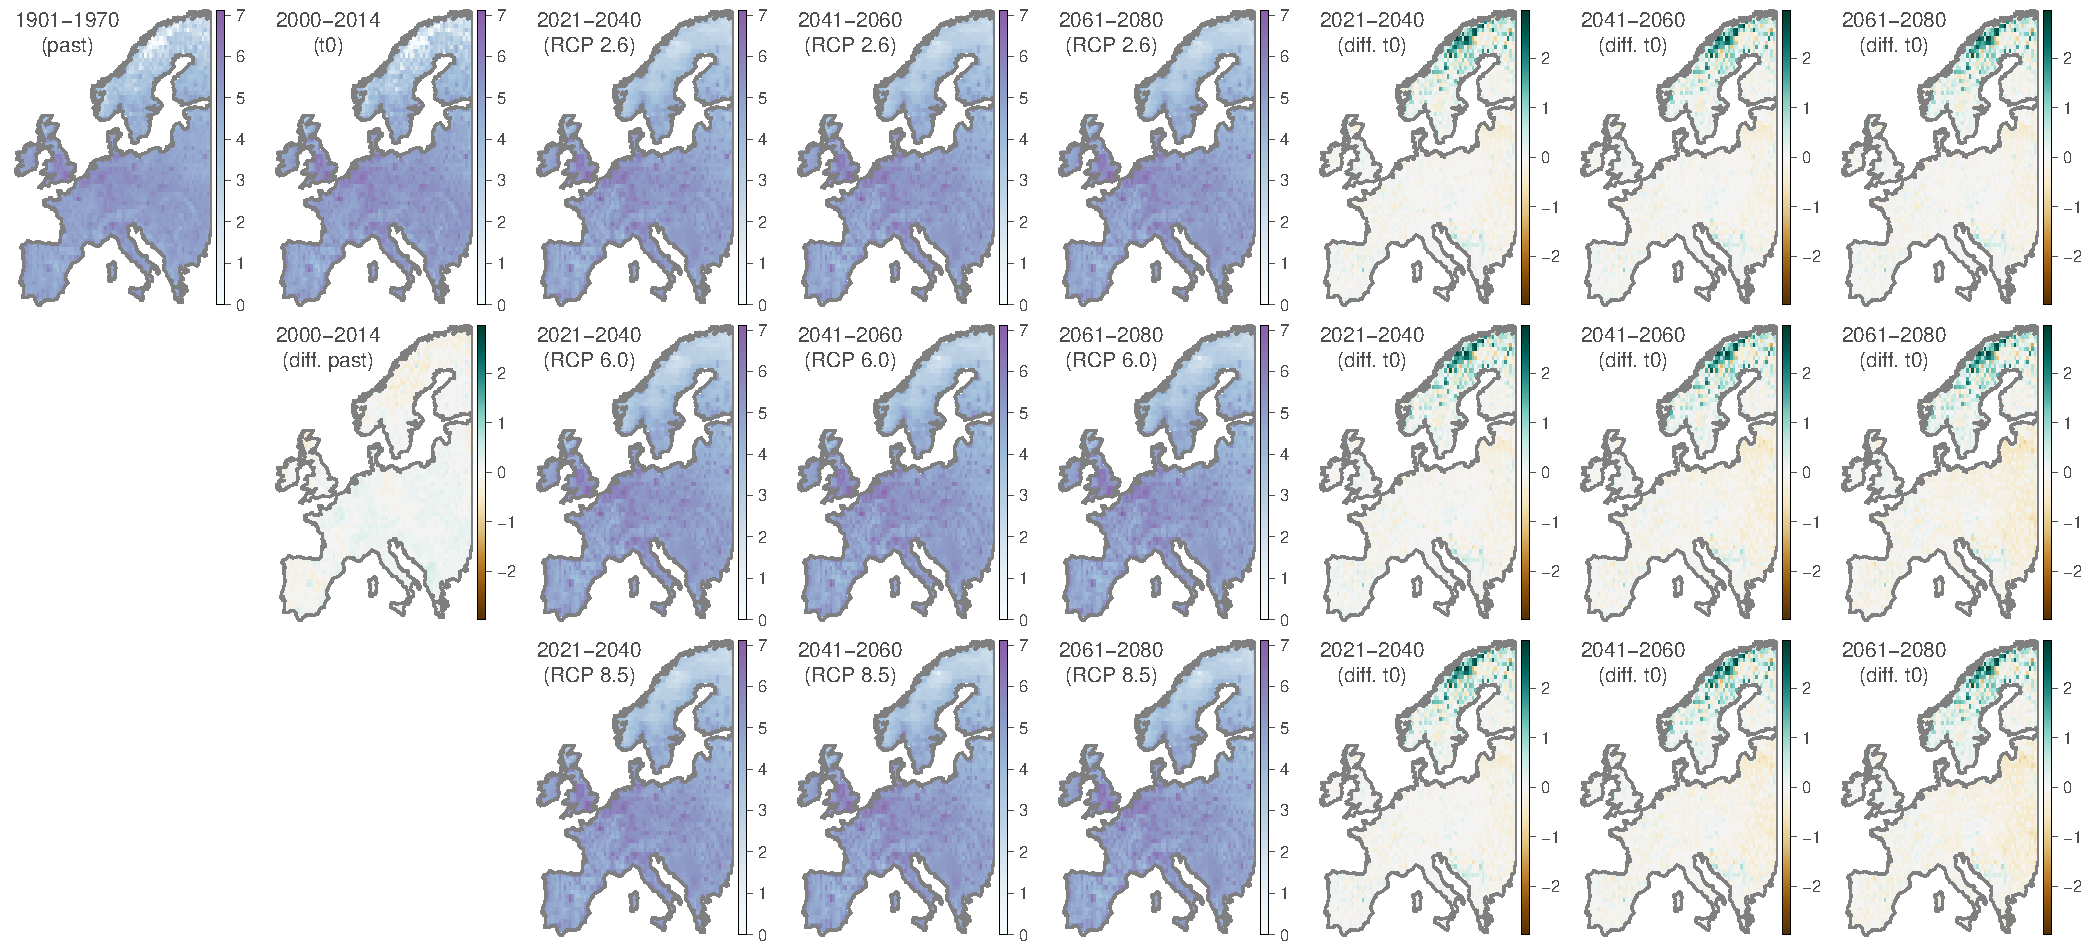
\includegraphics[width=1.00\textwidth]{Environmental_variable_9.pdf}}
\caption{\small{\textbf{9� environmental variable involved in ecological niche modelling: human population (log\textsubscript{10}-transformed).}
We here also report the difference between each future estimate and the estimate for the current period (t0).}}
\label{FigureS9}
\end{figure}

\renewcommand{\thefigure}{S10}
\begin{figure}[H]
\centering
\makebox[\textwidth][c]{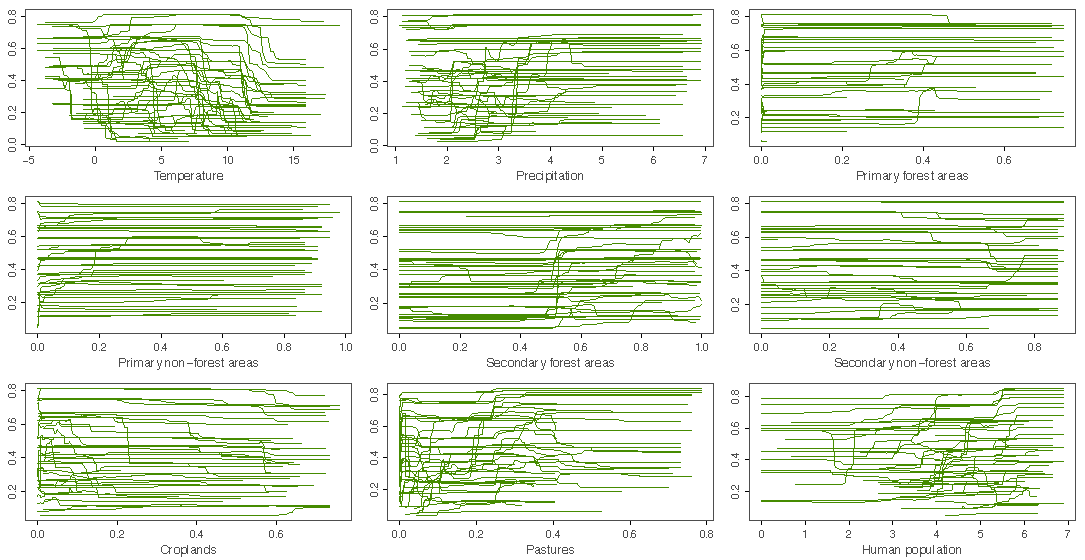
\includegraphics[width=1.01\textwidth]{All_response_curves_2.pdf}}
\caption{\small{\textbf{Response curves of environmental variables included in ecological niche models.}
}}
\label{FigureS10}
\end{figure}

\renewcommand{\thefigure}{S11}
\begin{figure}[H]
\centering
\makebox[\textwidth][c]{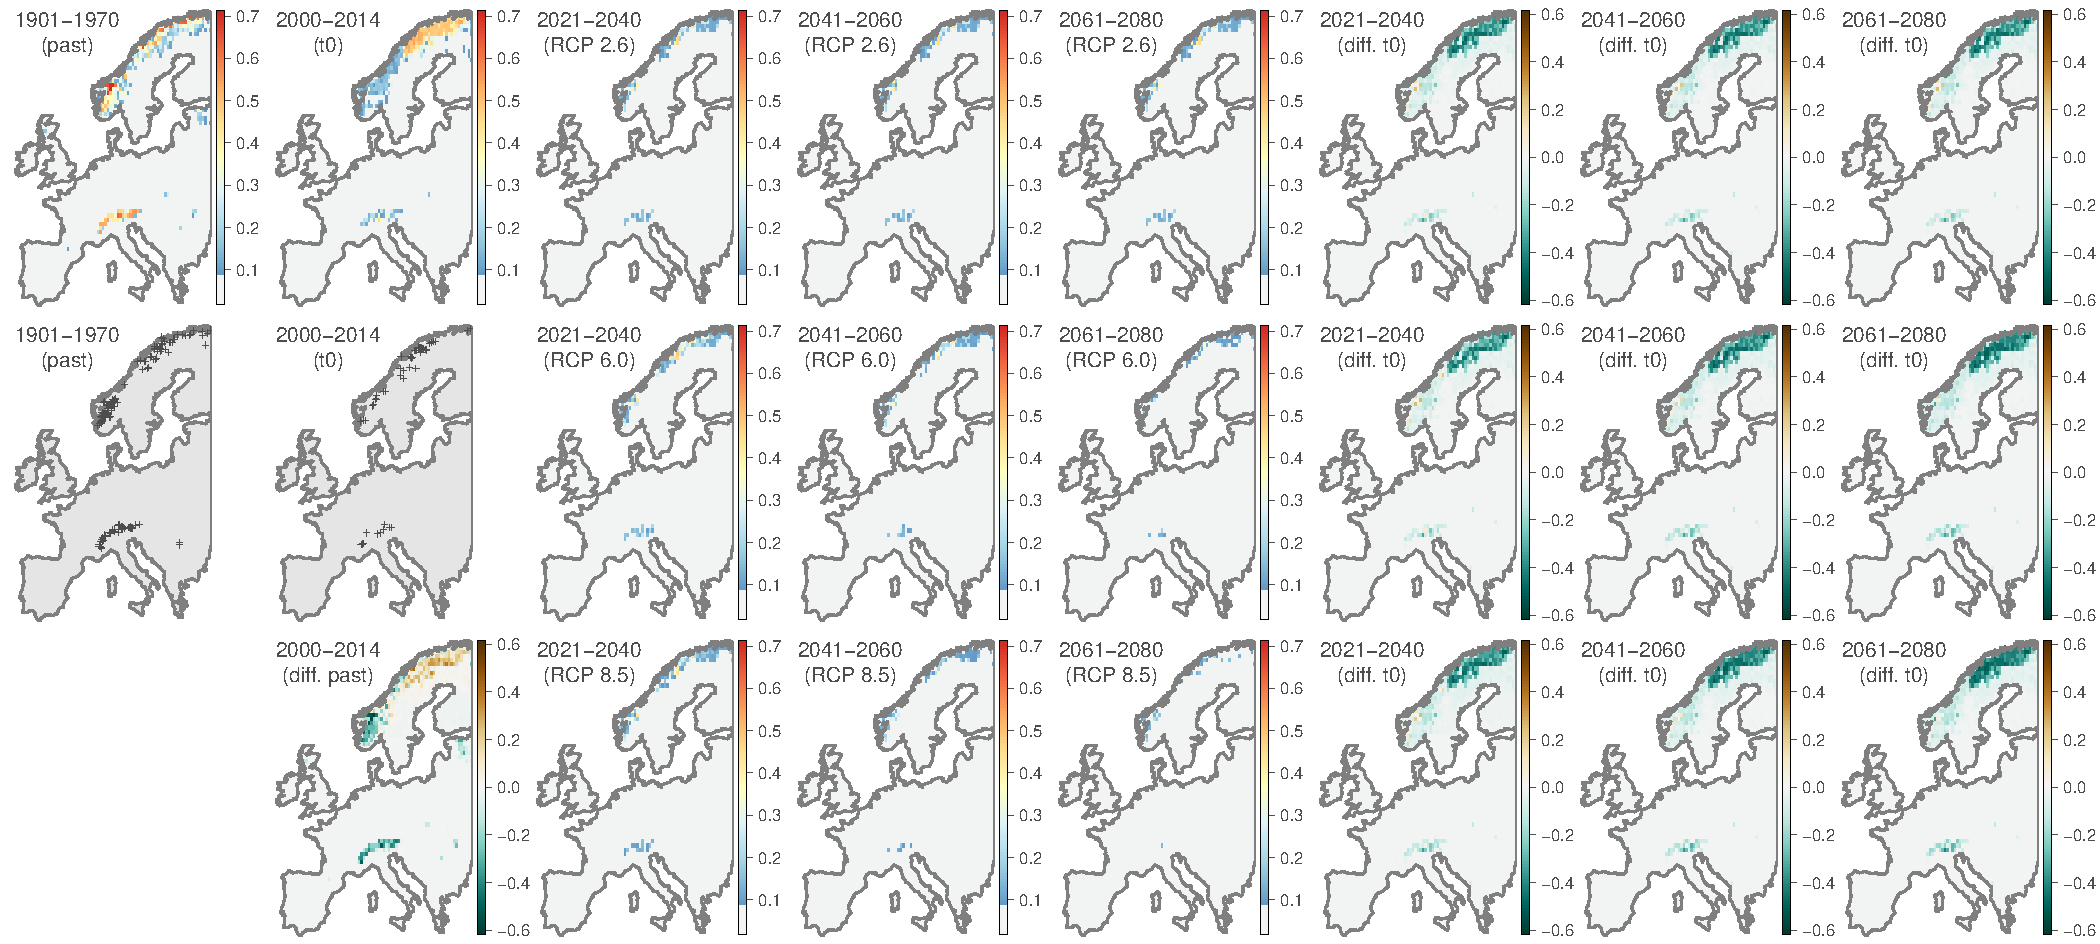
\includegraphics[width=1.00\textwidth]{All_the_species_projections/B_alpinus_projections.pdf}}
\caption{\small{\textbf{Ecological niche modelling for \emph{Bombus alpinus}.}
We report the projection for the current period as well as differences between future and current projections.}}
\label{FigureS11}
\end{figure}
\renewcommand{\thefigure}{S12}
\begin{figure}[H]
\centering
\makebox[\textwidth][c]{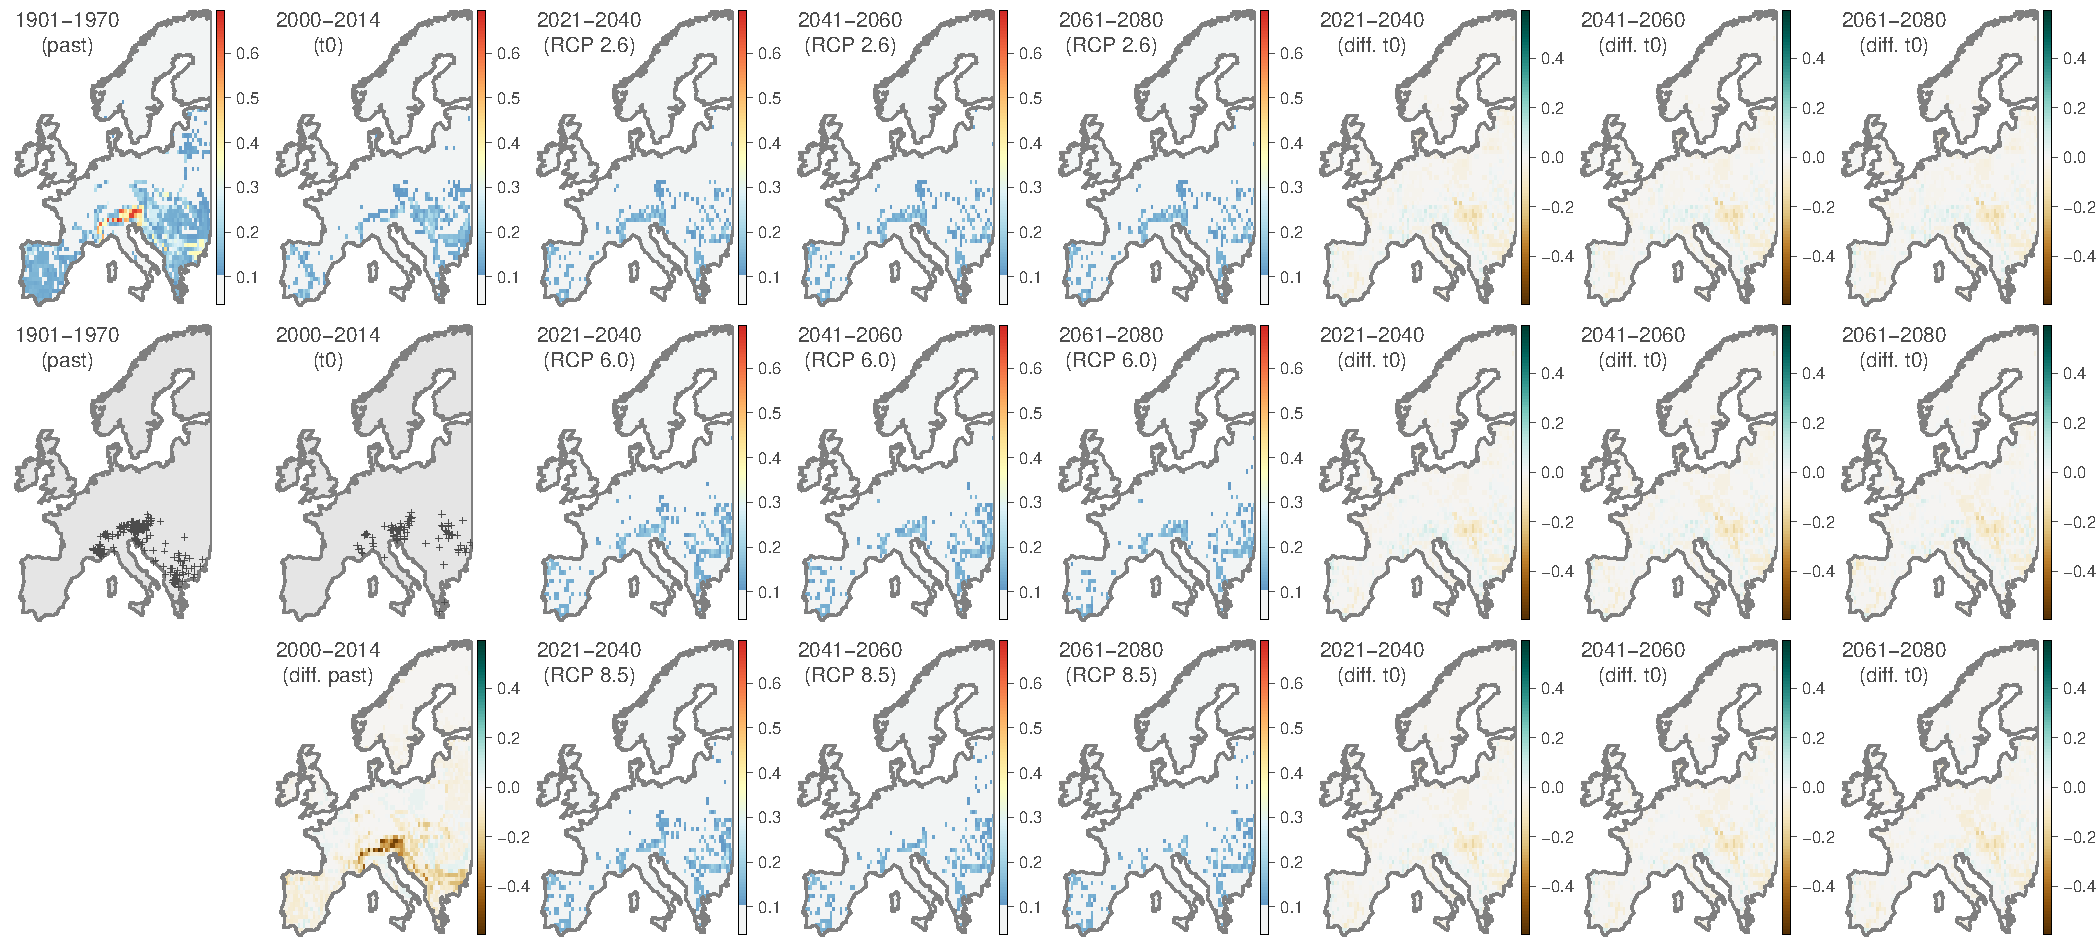
\includegraphics[width=1.00\textwidth]{All_the_species_projections/B_argillaceus_projections.pdf}}
\caption{\small{\textbf{Ecological niche modelling for \emph{Bombus argillaceus}.}
We report the projection for the current period as well as differences between future and current projections.}}
\label{FigureS12}
\end{figure}
\renewcommand{\thefigure}{S13}
\begin{figure}[H]
\centering
\makebox[\textwidth][c]{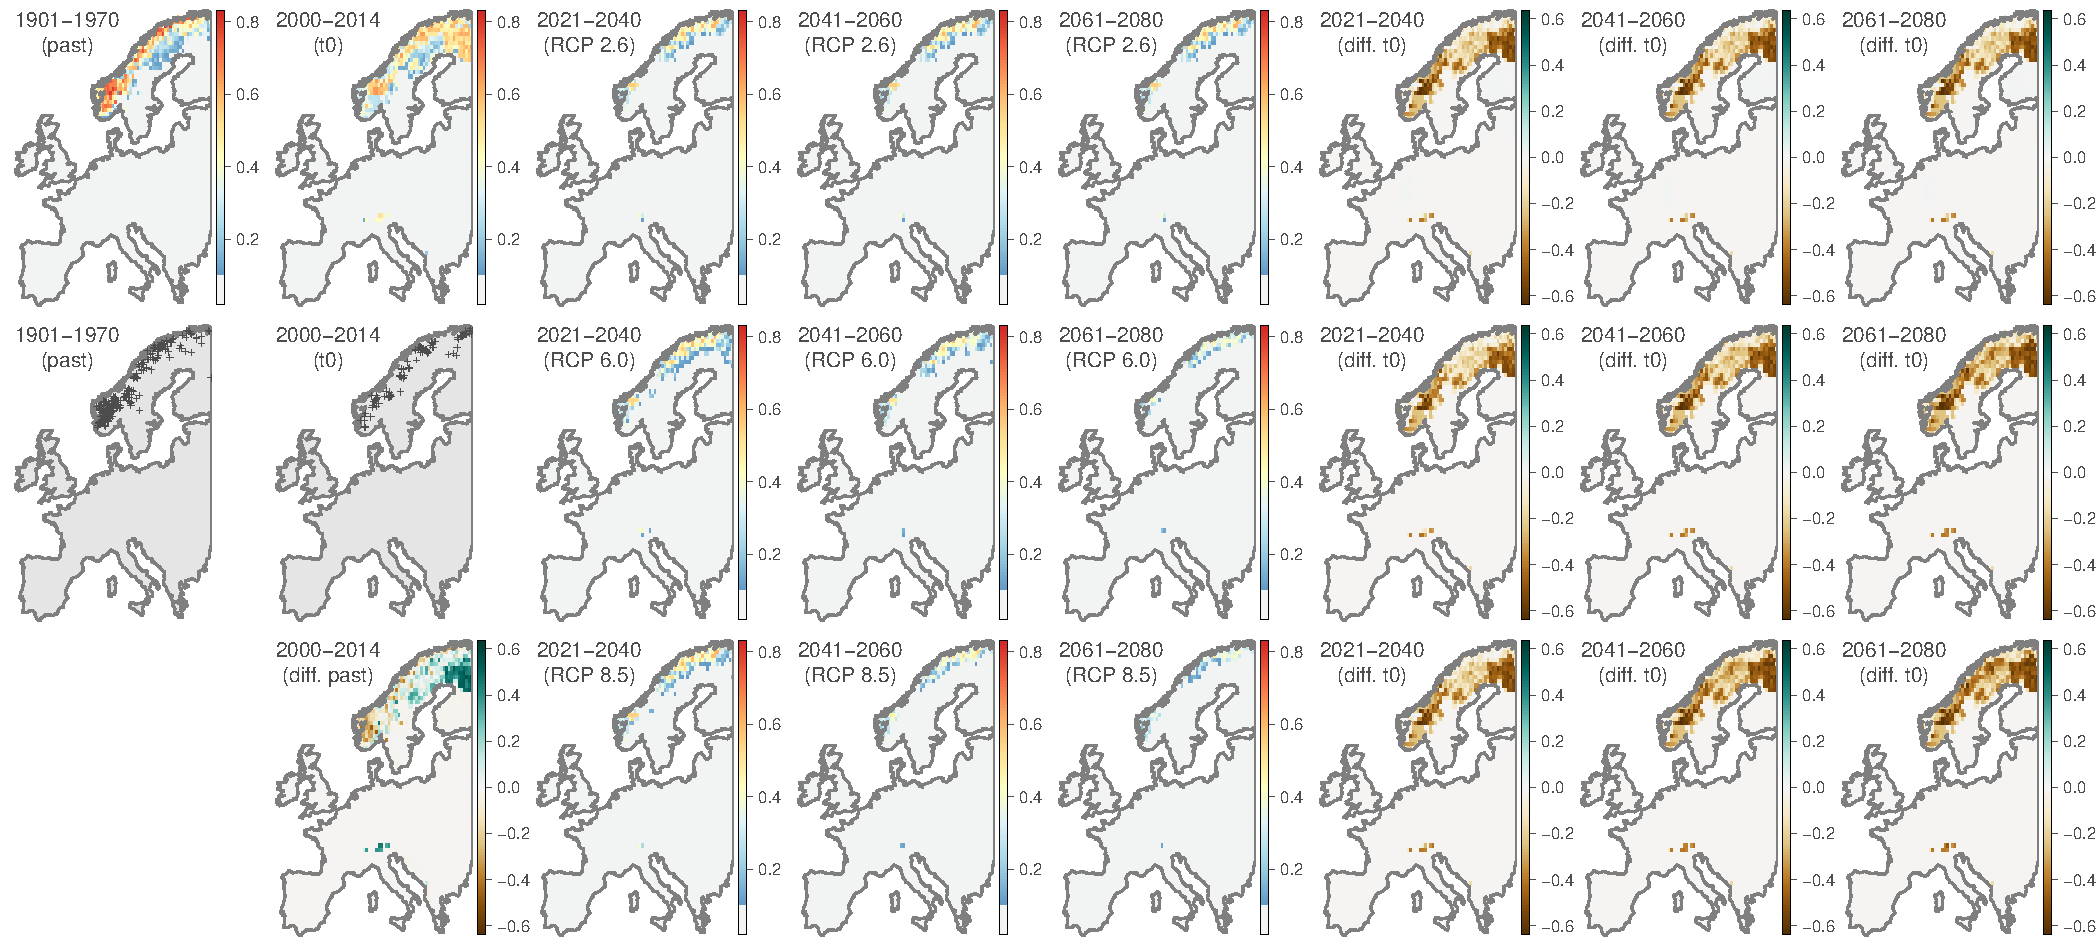
\includegraphics[width=1.00\textwidth]{All_the_species_projections/B_balteatus_projections.pdf}}
\caption{\small{\textbf{Ecological niche modelling for \emph{Bombus balteatus}.}
We report the projection for the current period as well as differences between future and current projections.}}
\label{FigureS13}
\end{figure}
\renewcommand{\thefigure}{S14}
\begin{figure}[H]
\centering
\makebox[\textwidth][c]{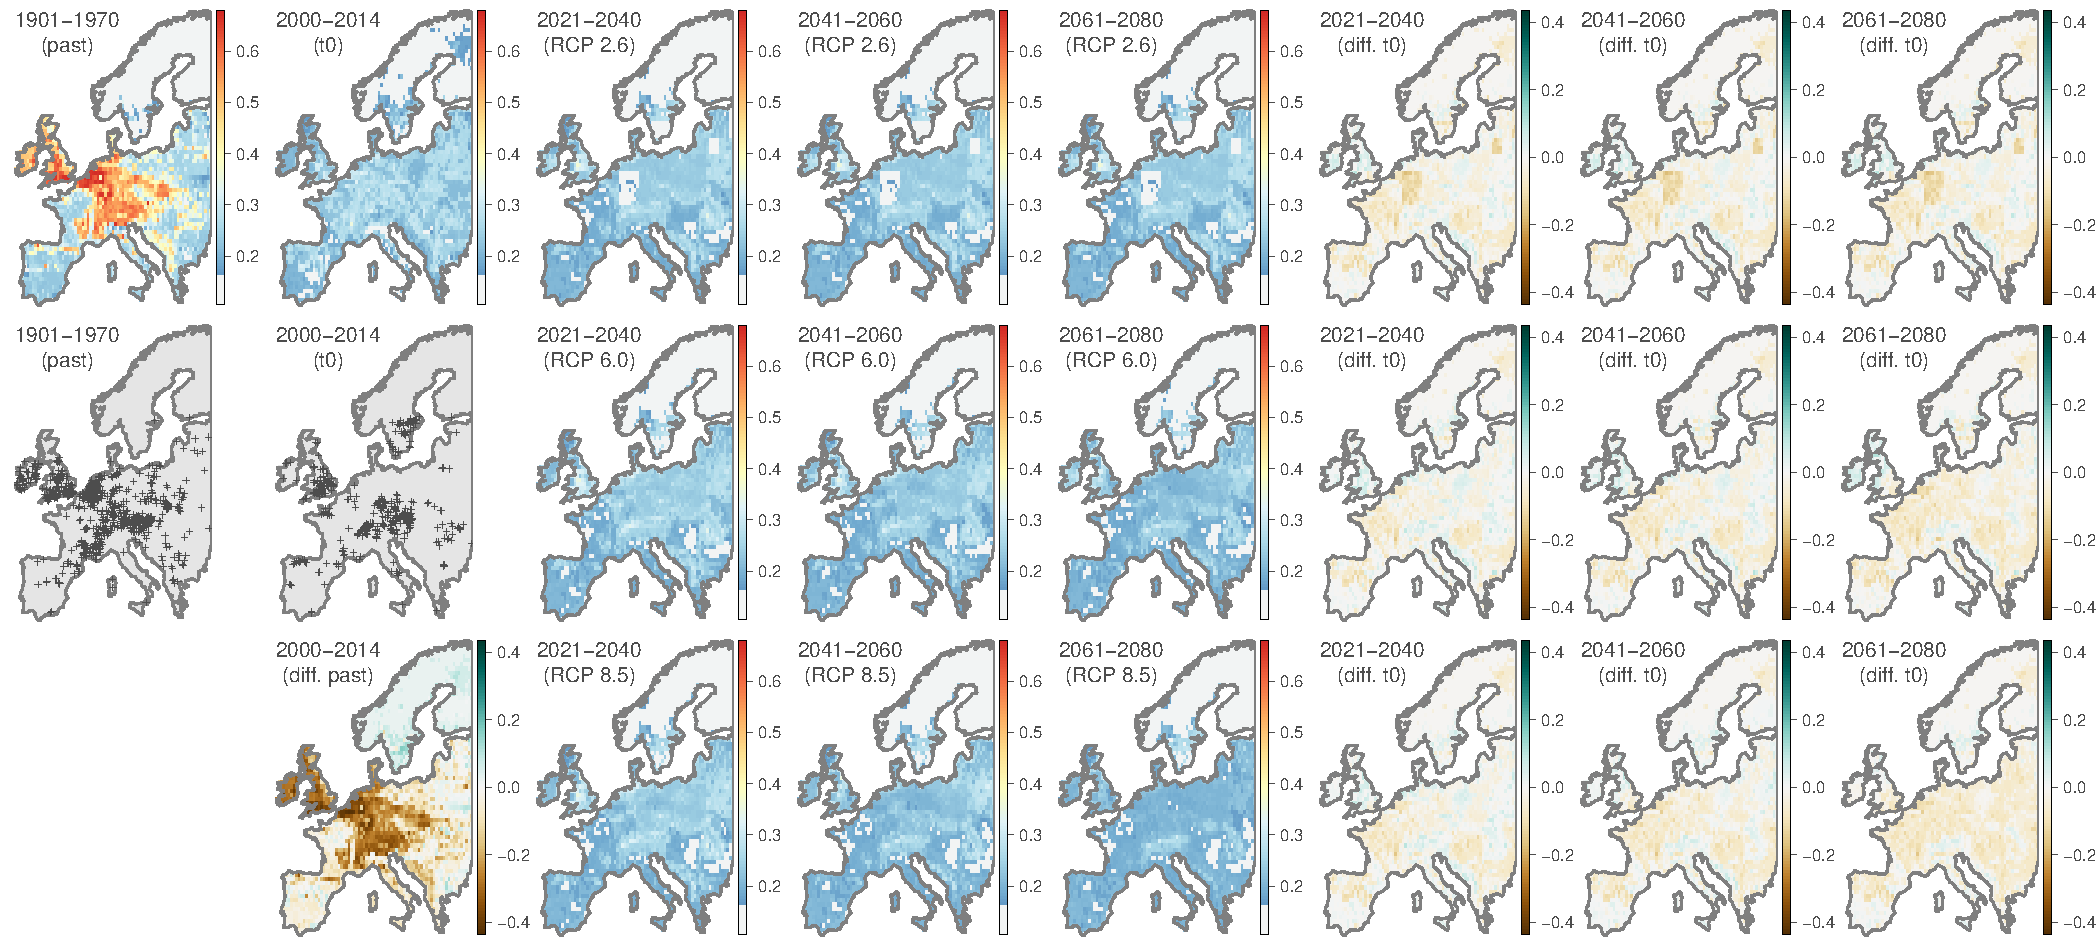
\includegraphics[width=1.00\textwidth]{All_the_species_projections/B_barbutellus_projections.pdf}}
\caption{\small{\textbf{Ecological niche modelling for \emph{Bombus barbutellus}.}
We report the projection for the current period as well as differences between future and current projections.}}
\label{FigureS14}
\end{figure}
\renewcommand{\thefigure}{S15}
\begin{figure}[H]
\centering
\makebox[\textwidth][c]{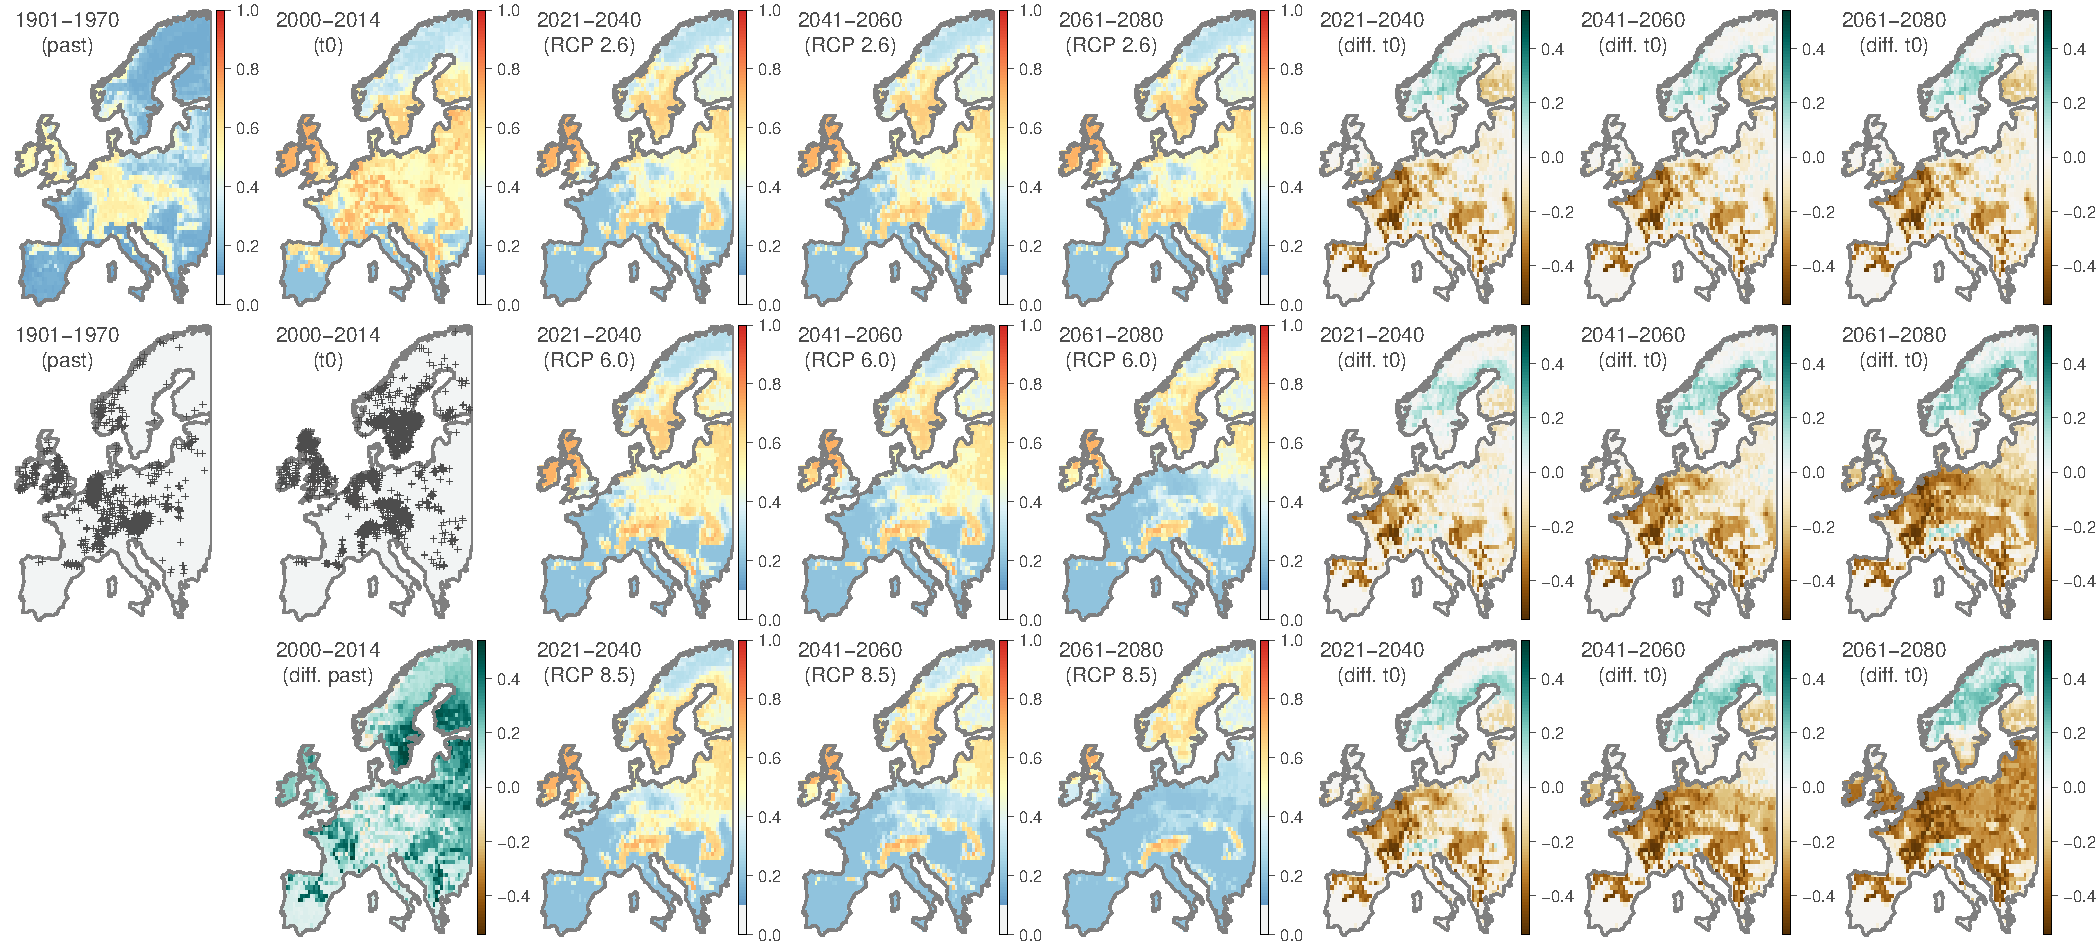
\includegraphics[width=1.00\textwidth]{All_the_species_projections/B_bohemicus_projections.pdf}}
\caption{\small{\textbf{Ecological niche modelling for \emph{Bombus bohemicus}.}
We report the projection for the current period as well as differences between future and current projections.}}
\label{FigureS15}
\end{figure}
\renewcommand{\thefigure}{S16}
\begin{figure}[H]
\centering
\makebox[\textwidth][c]{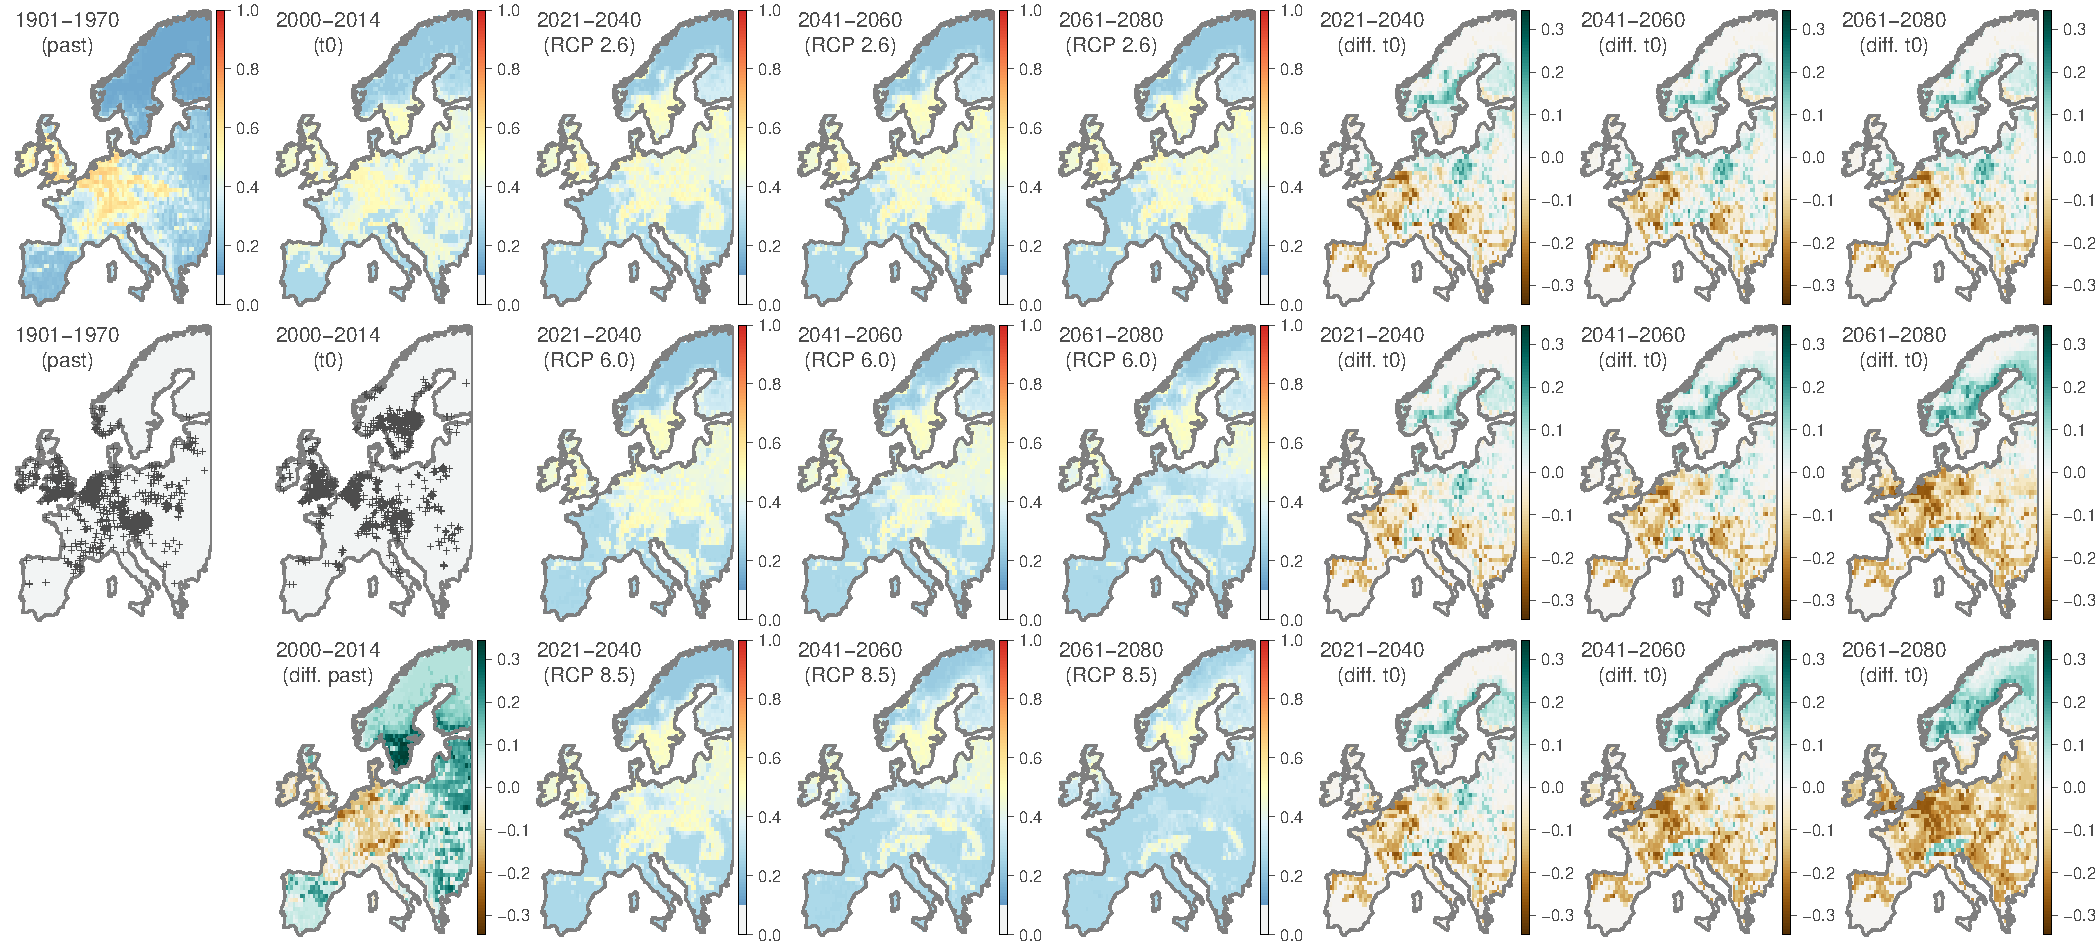
\includegraphics[width=1.00\textwidth]{All_the_species_projections/B_campestris_projections.pdf}}
\caption{\small{\textbf{Ecological niche modelling for \emph{Bombus campestris}.}
We report the projection for the current period as well as differences between future and current projections.}}
\label{FigureS16}
\end{figure}
\renewcommand{\thefigure}{S17}
\begin{figure}[H]
\centering
\makebox[\textwidth][c]{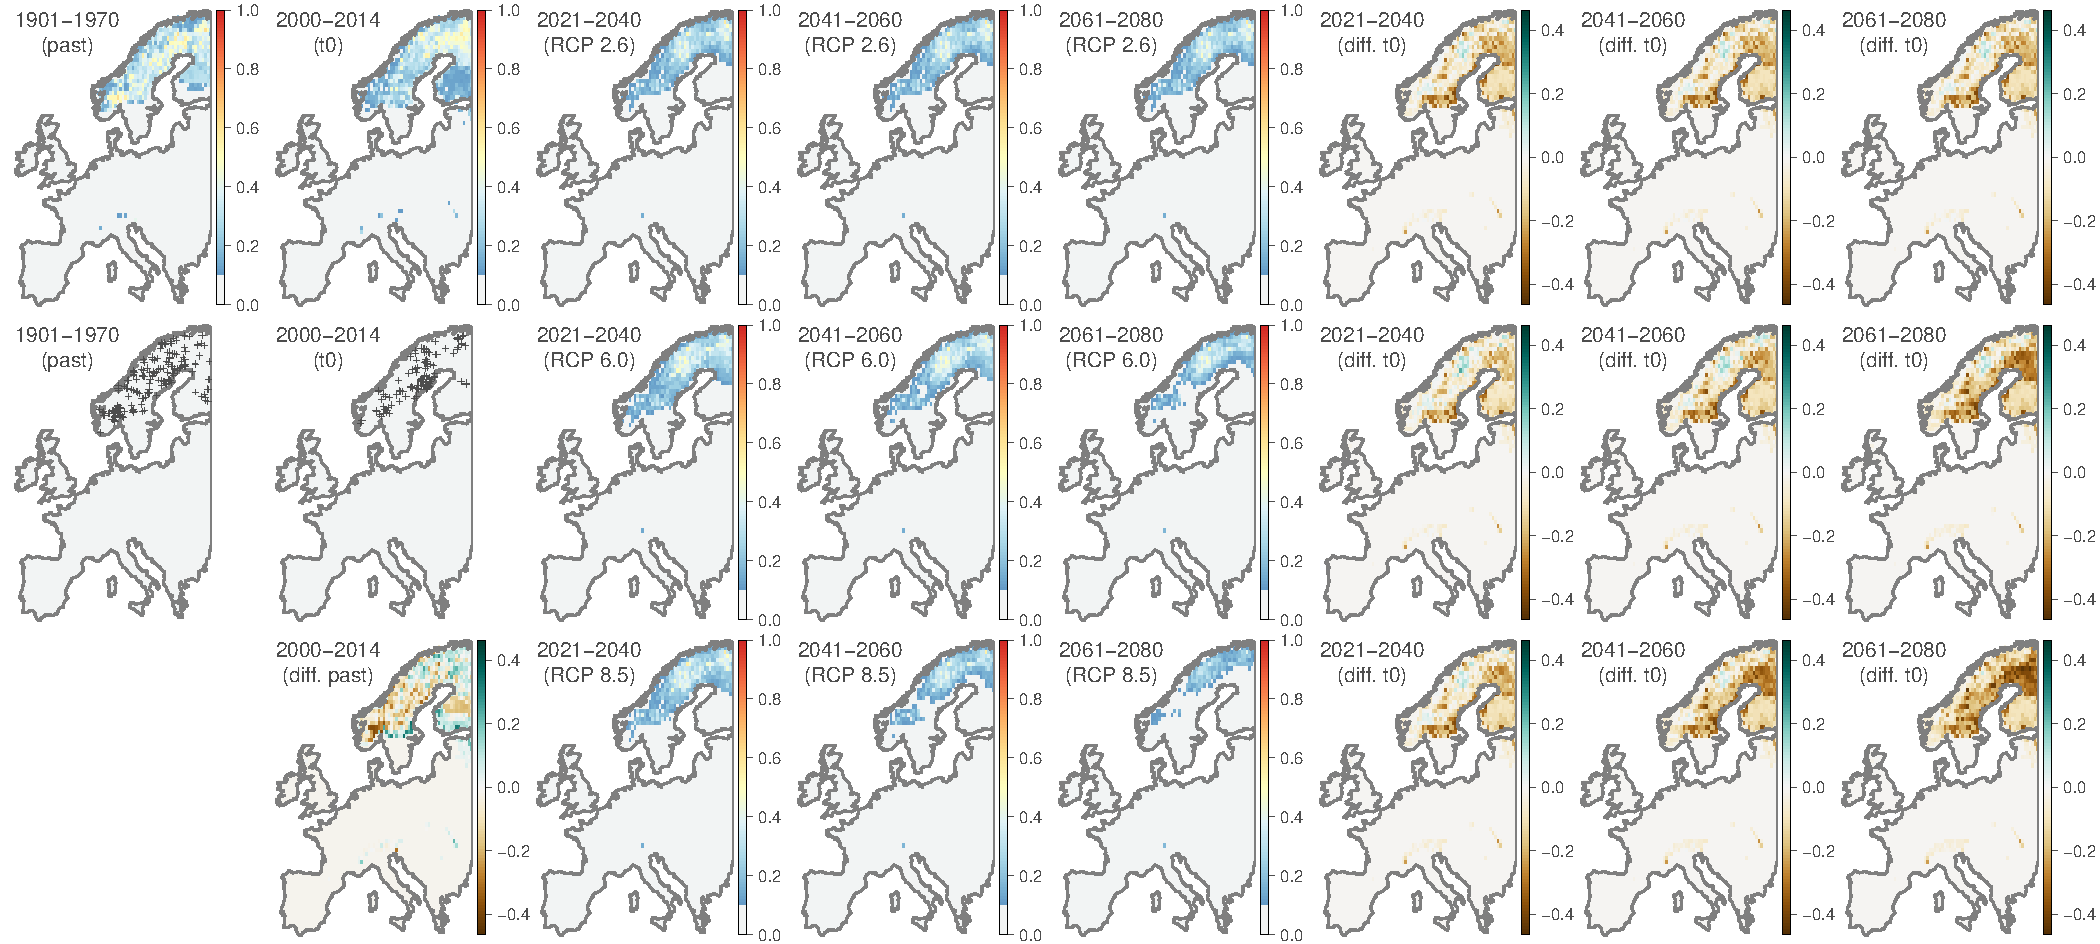
\includegraphics[width=1.00\textwidth]{All_the_species_projections/B_cingulatus_projections.pdf}}
\caption{\small{\textbf{Ecological niche modelling for \emph{Bombus cingulatus}.}
We report the projection for the current period as well as differences between future and current projections.}}
\label{FigureS17}
\end{figure}
\renewcommand{\thefigure}{S18}
\begin{figure}[H]
\centering
\makebox[\textwidth][c]{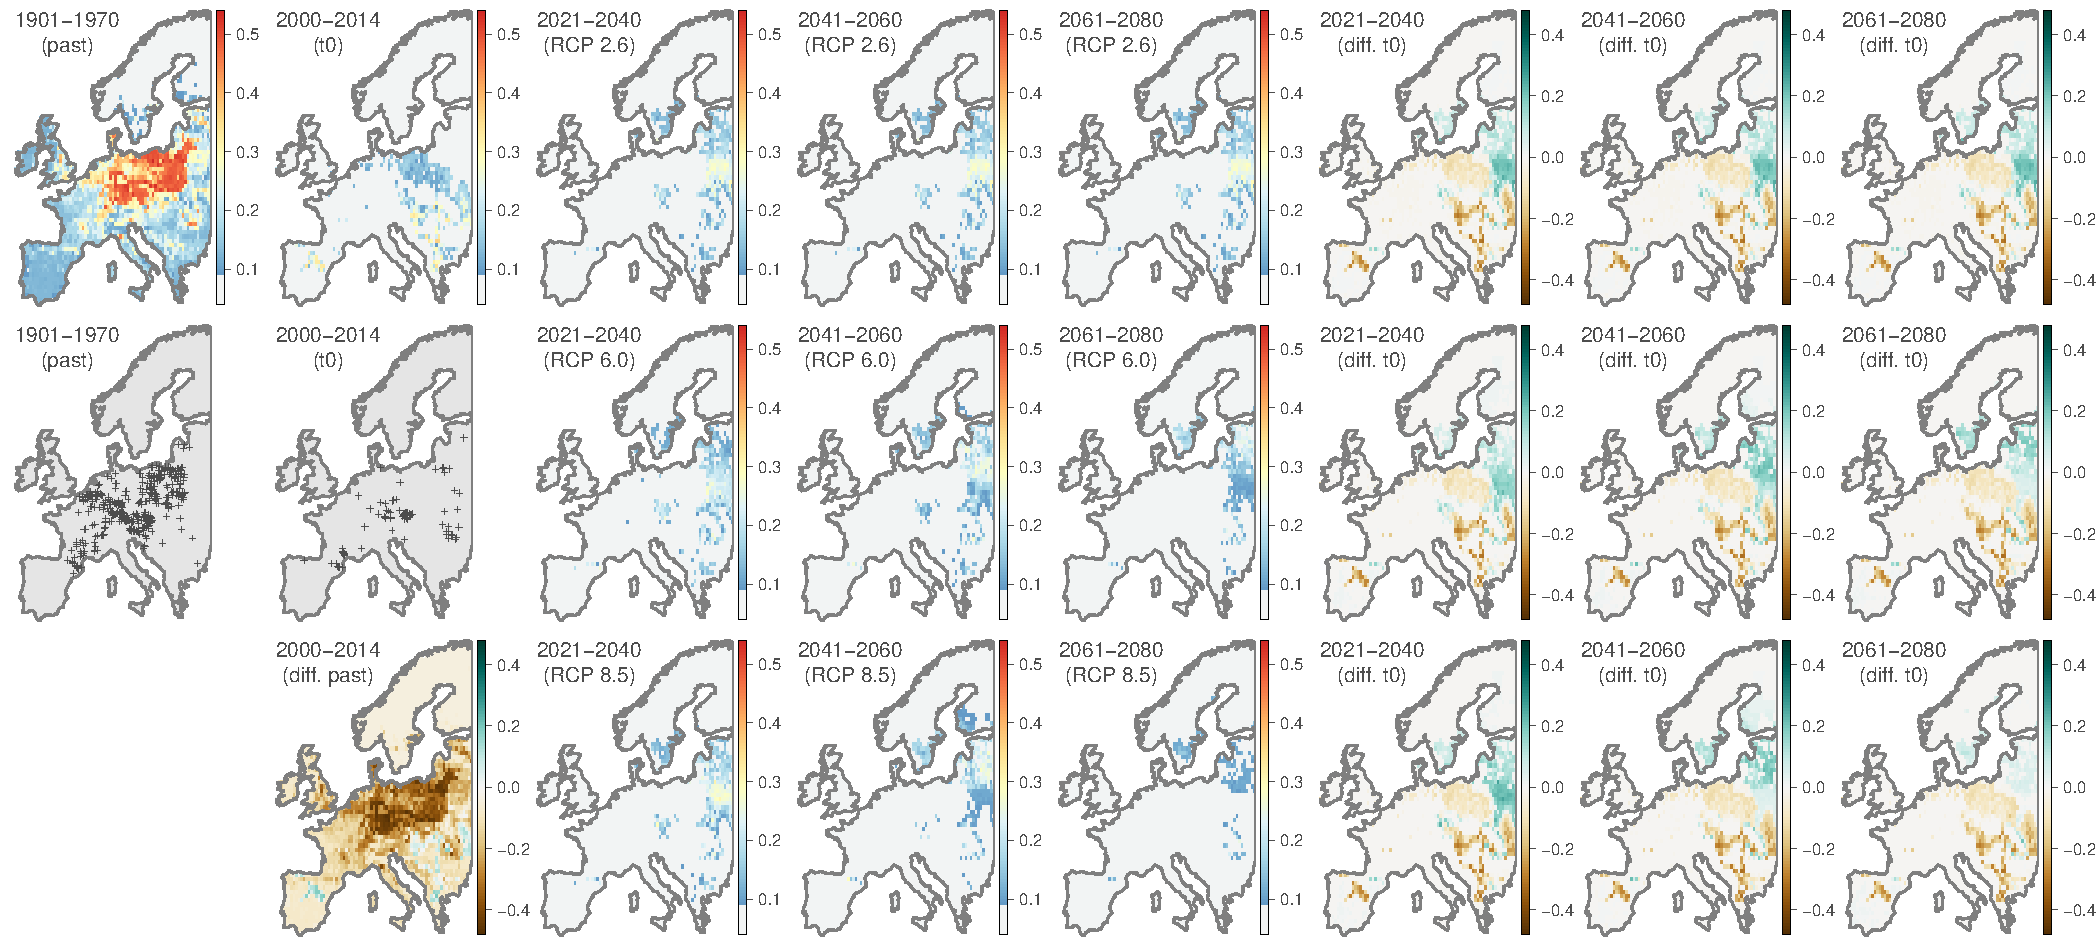
\includegraphics[width=1.00\textwidth]{All_the_species_projections/B_confusus_projections.pdf}}
\caption{\small{\textbf{Ecological niche modelling for \emph{Bombus confusus}.}
We report the projection for the current period as well as differences between future and current projections.}}
\label{FigureS18}
\end{figure}
\renewcommand{\thefigure}{S19}
\begin{figure}[H]
\centering
\makebox[\textwidth][c]{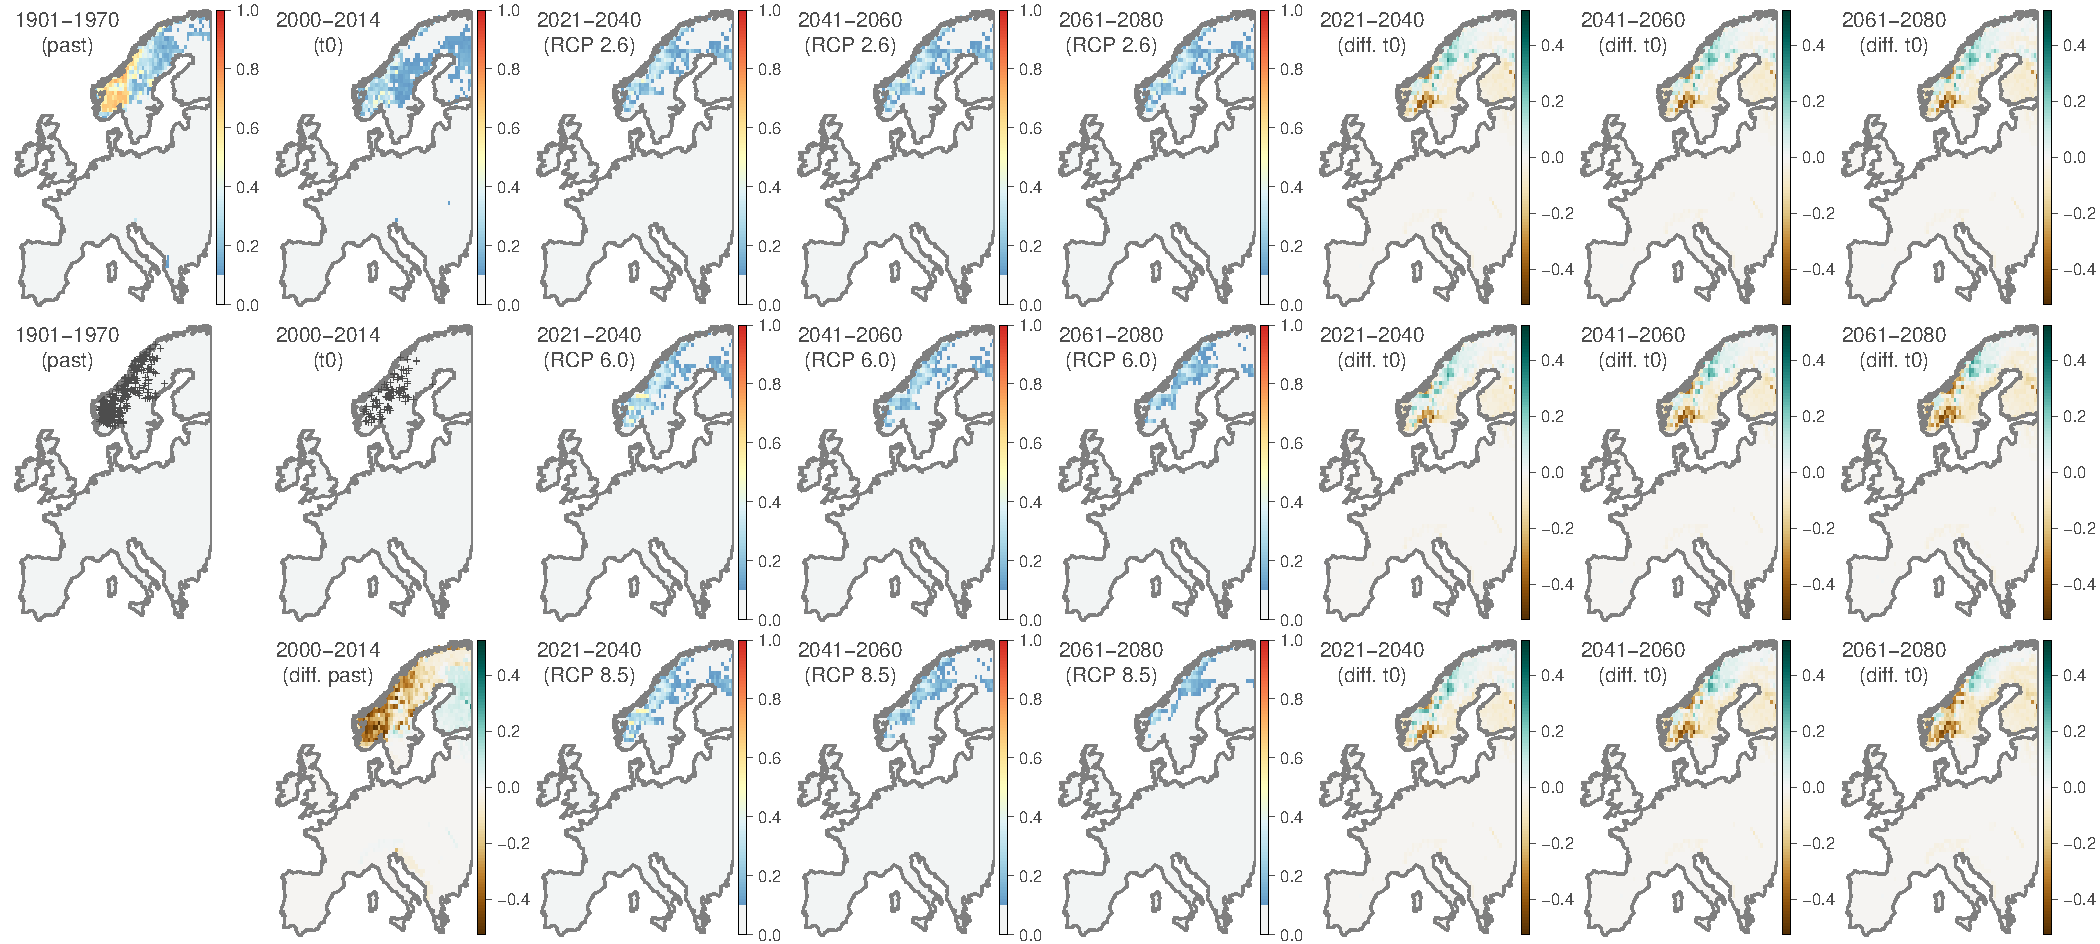
\includegraphics[width=1.00\textwidth]{All_the_species_projections/B_consobrinus_projections.pdf}}
\caption{\small{\textbf{Ecological niche modelling for \emph{Bombus consobrinus}.}
We report the projection for the current period as well as differences between future and current projections.}}
\label{FigureS19}
\end{figure}
\renewcommand{\thefigure}{S20}
\begin{figure}[H]
\centering
\makebox[\textwidth][c]{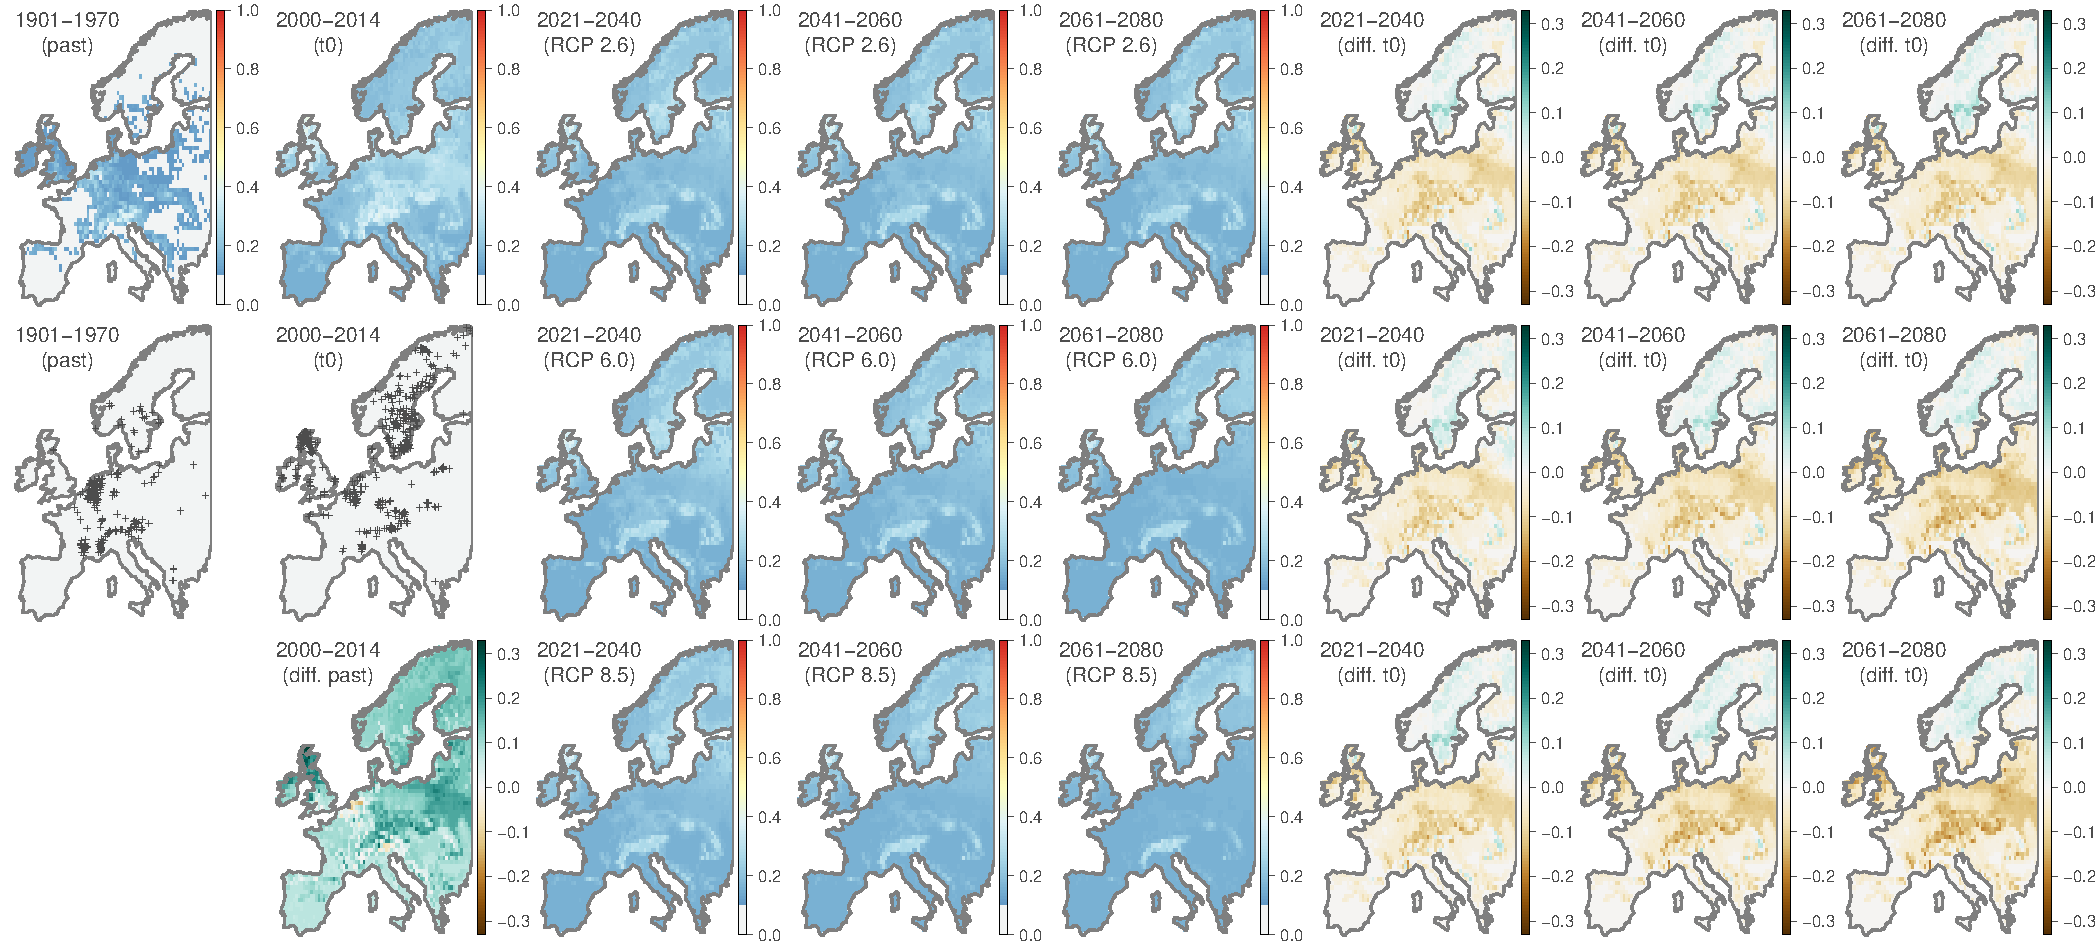
\includegraphics[width=1.00\textwidth]{All_the_species_projections/B_cryptarum_projections.pdf}}
\caption{\small{\textbf{Ecological niche modelling for \emph{Bombus cryptarum}.}
We report the projection for the current period as well as differences between future and current projections.}}
\label{FigureS20}
\end{figure}
\renewcommand{\thefigure}{S21}
\begin{figure}[H]
\centering
\makebox[\textwidth][c]{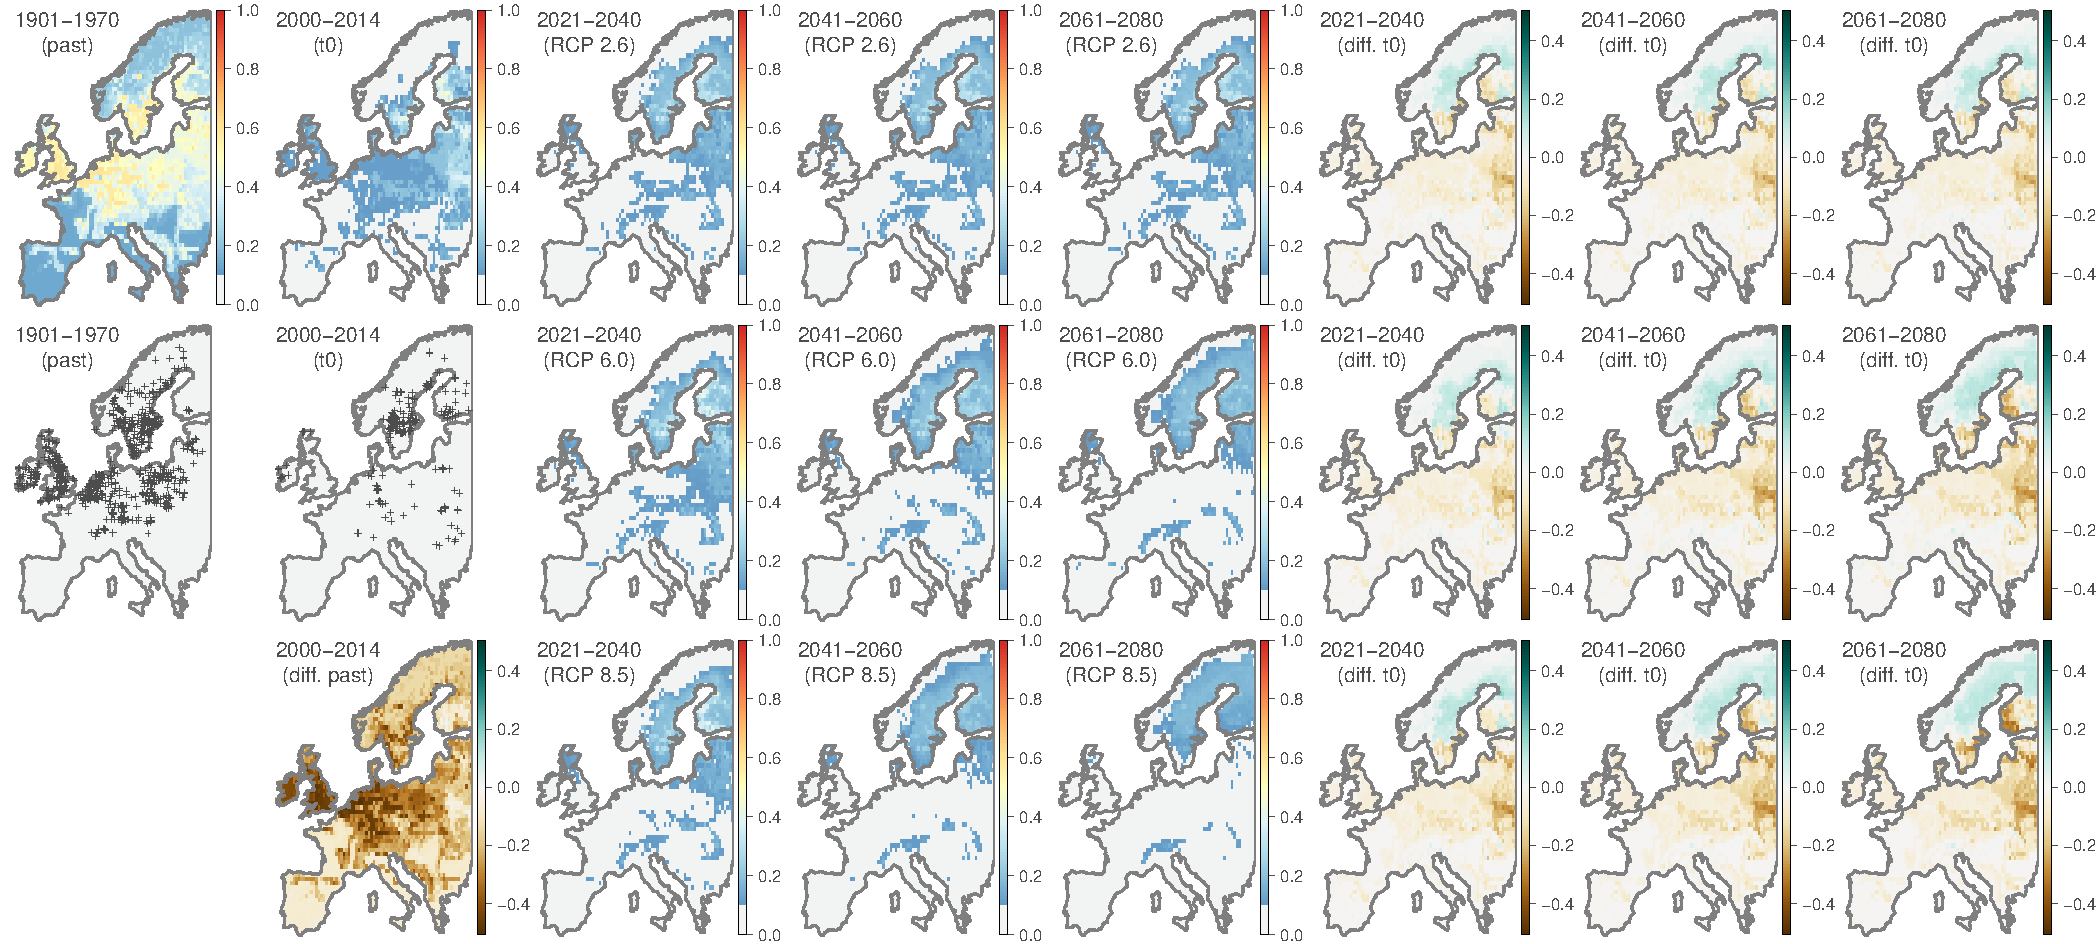
\includegraphics[width=1.00\textwidth]{All_the_species_projections/B_distinguendus_projections.pdf}}
\caption{\small{\textbf{Ecological niche modelling for \emph{Bombus distinguendus}.}
We report the projection for the current period as well as differences between future and current projections.}}
\label{FigureS21}
\end{figure}
\renewcommand{\thefigure}{S22}
\begin{figure}[H]
\centering
\makebox[\textwidth][c]{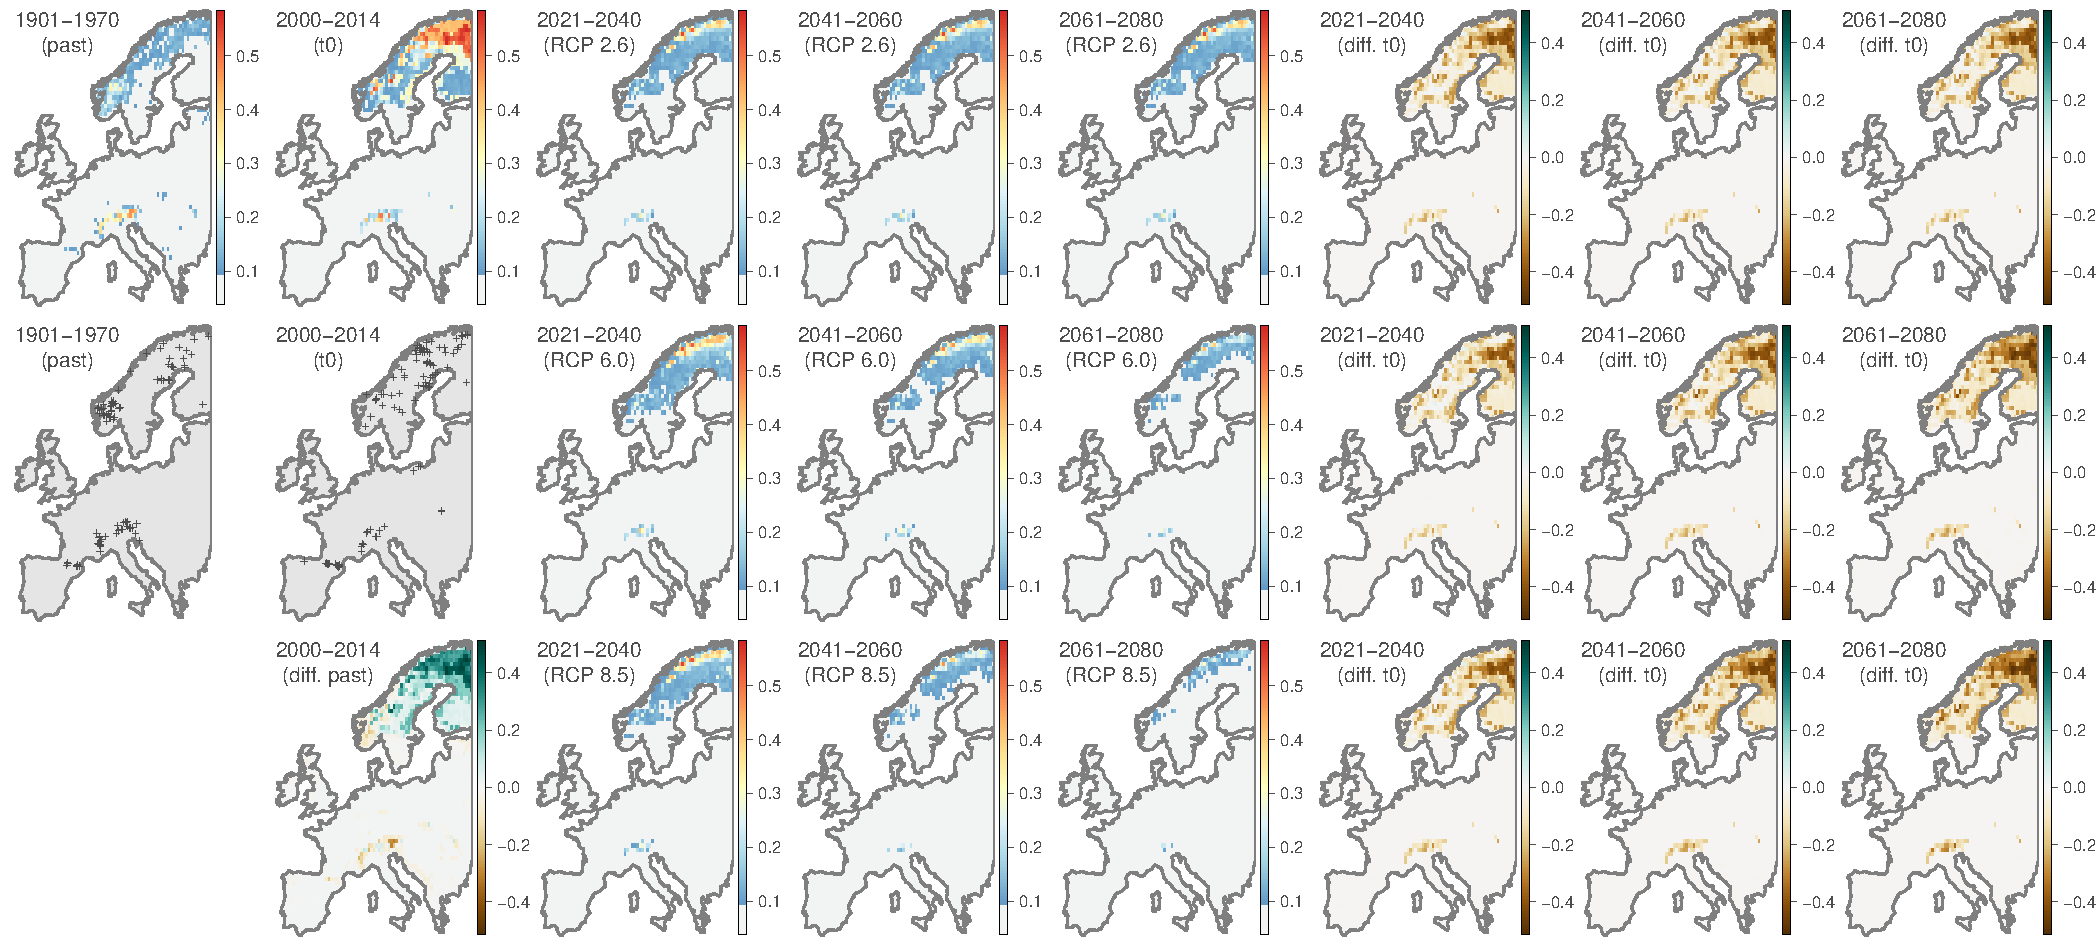
\includegraphics[width=1.00\textwidth]{All_the_species_projections/B_flavidus_projections.pdf}}
\caption{\small{\textbf{Ecological niche modelling for \emph{Bombus flavidus}.}
We report the projection for the current period as well as differences between future and current projections.}}
\label{FigureS22}
\end{figure}
\renewcommand{\thefigure}{S23}
\begin{figure}[H]
\centering
\makebox[\textwidth][c]{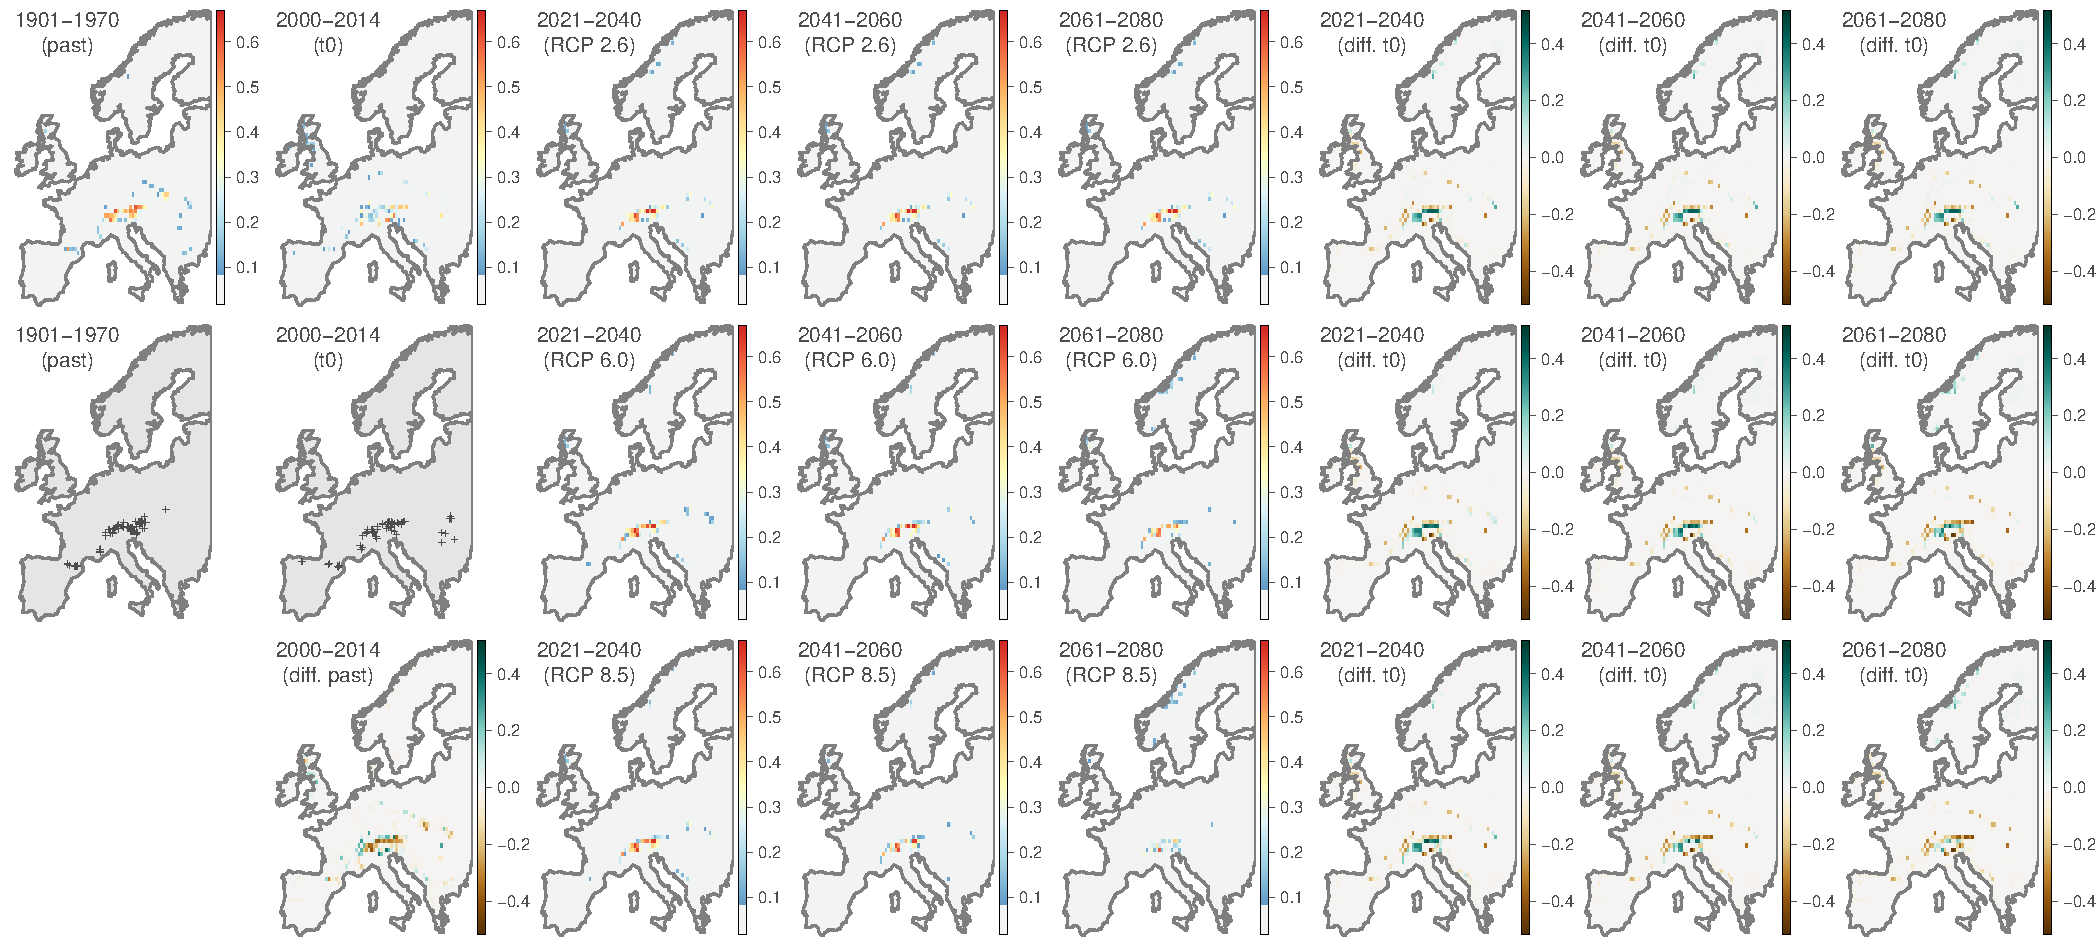
\includegraphics[width=1.00\textwidth]{All_the_species_projections/B_gerstaeckeri_projections.pdf}}
\caption{\small{\textbf{Ecological niche modelling for \emph{Bombus gerstaeckeri}.}
We report the projection for the current period as well as differences between future and current projections.}}
\label{FigureS23}
\end{figure}
\renewcommand{\thefigure}{S24}
\begin{figure}[H]
\centering
\makebox[\textwidth][c]{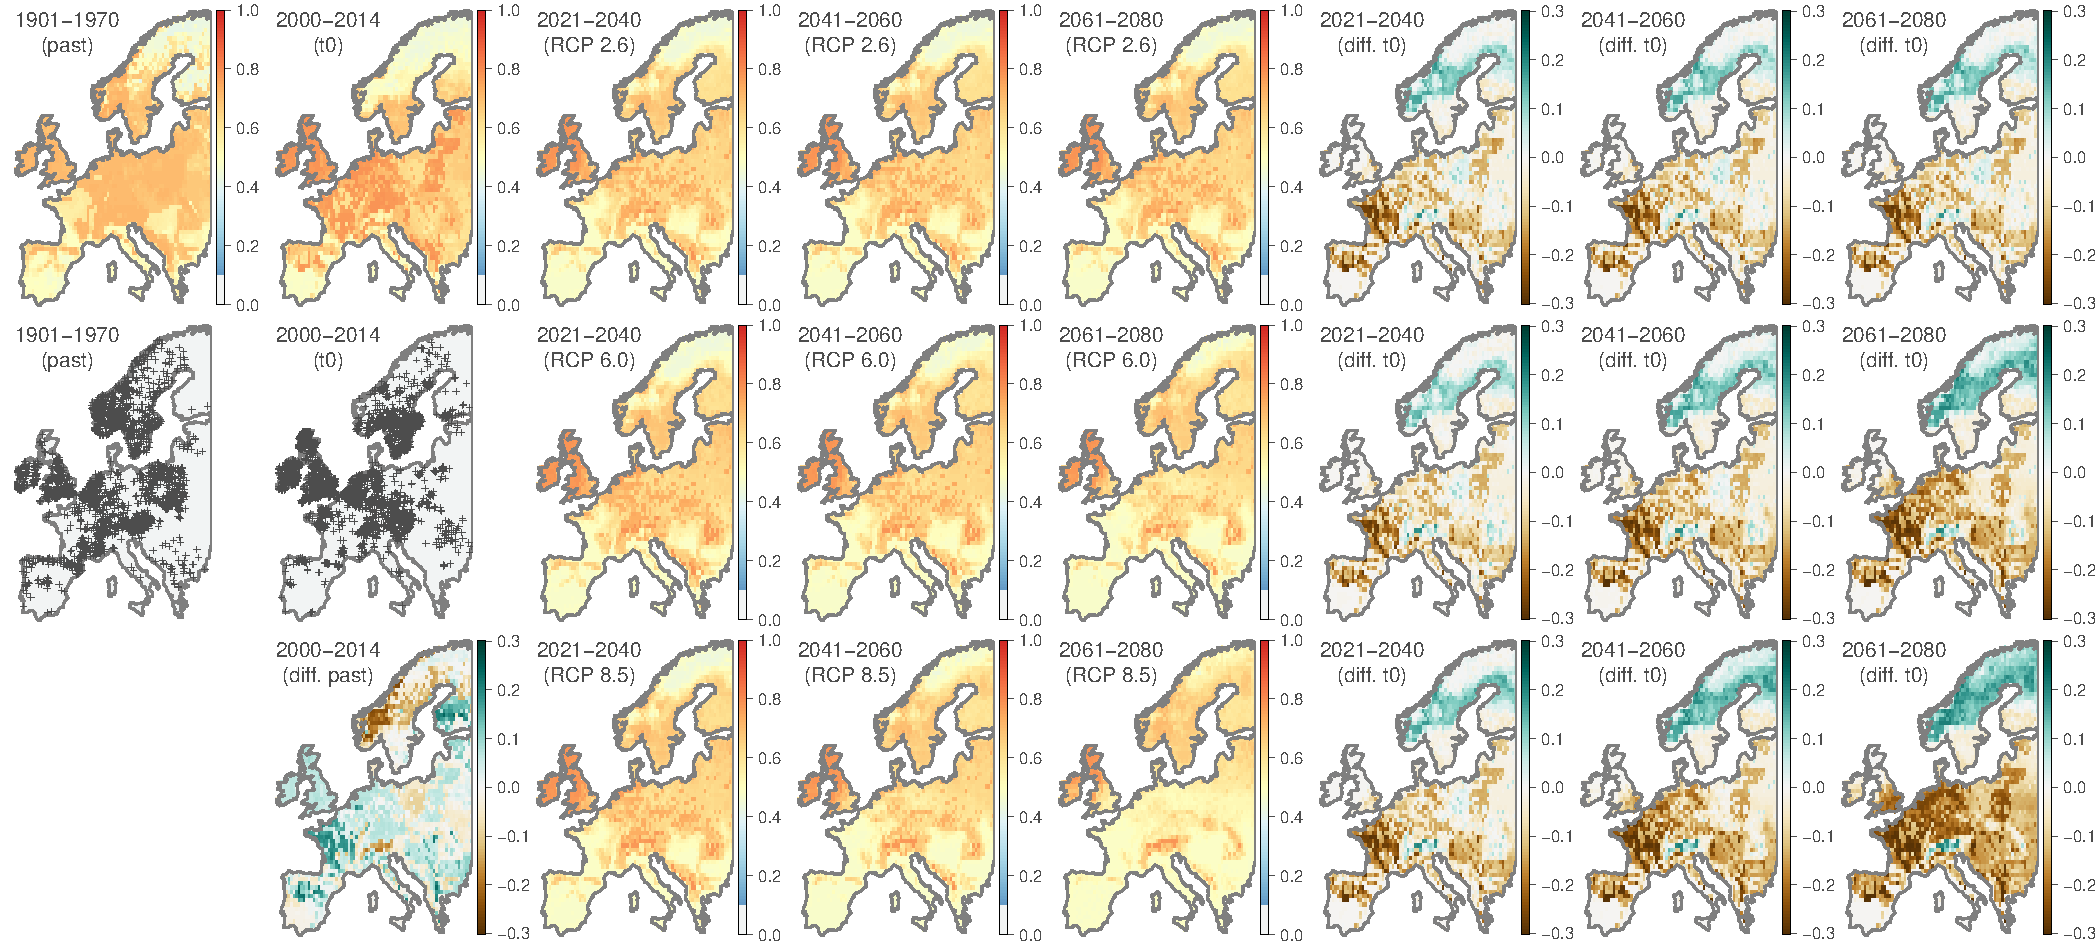
\includegraphics[width=1.00\textwidth]{All_the_species_projections/B_hortorum_projections.pdf}}
\caption{\small{\textbf{Ecological niche modelling for \emph{Bombus hortorum}.}
We report the projection for the current period as well as differences between future and current projections.}}
\label{FigureS24}
\end{figure}
\renewcommand{\thefigure}{S25}
\begin{figure}[H]
\centering
\makebox[\textwidth][c]{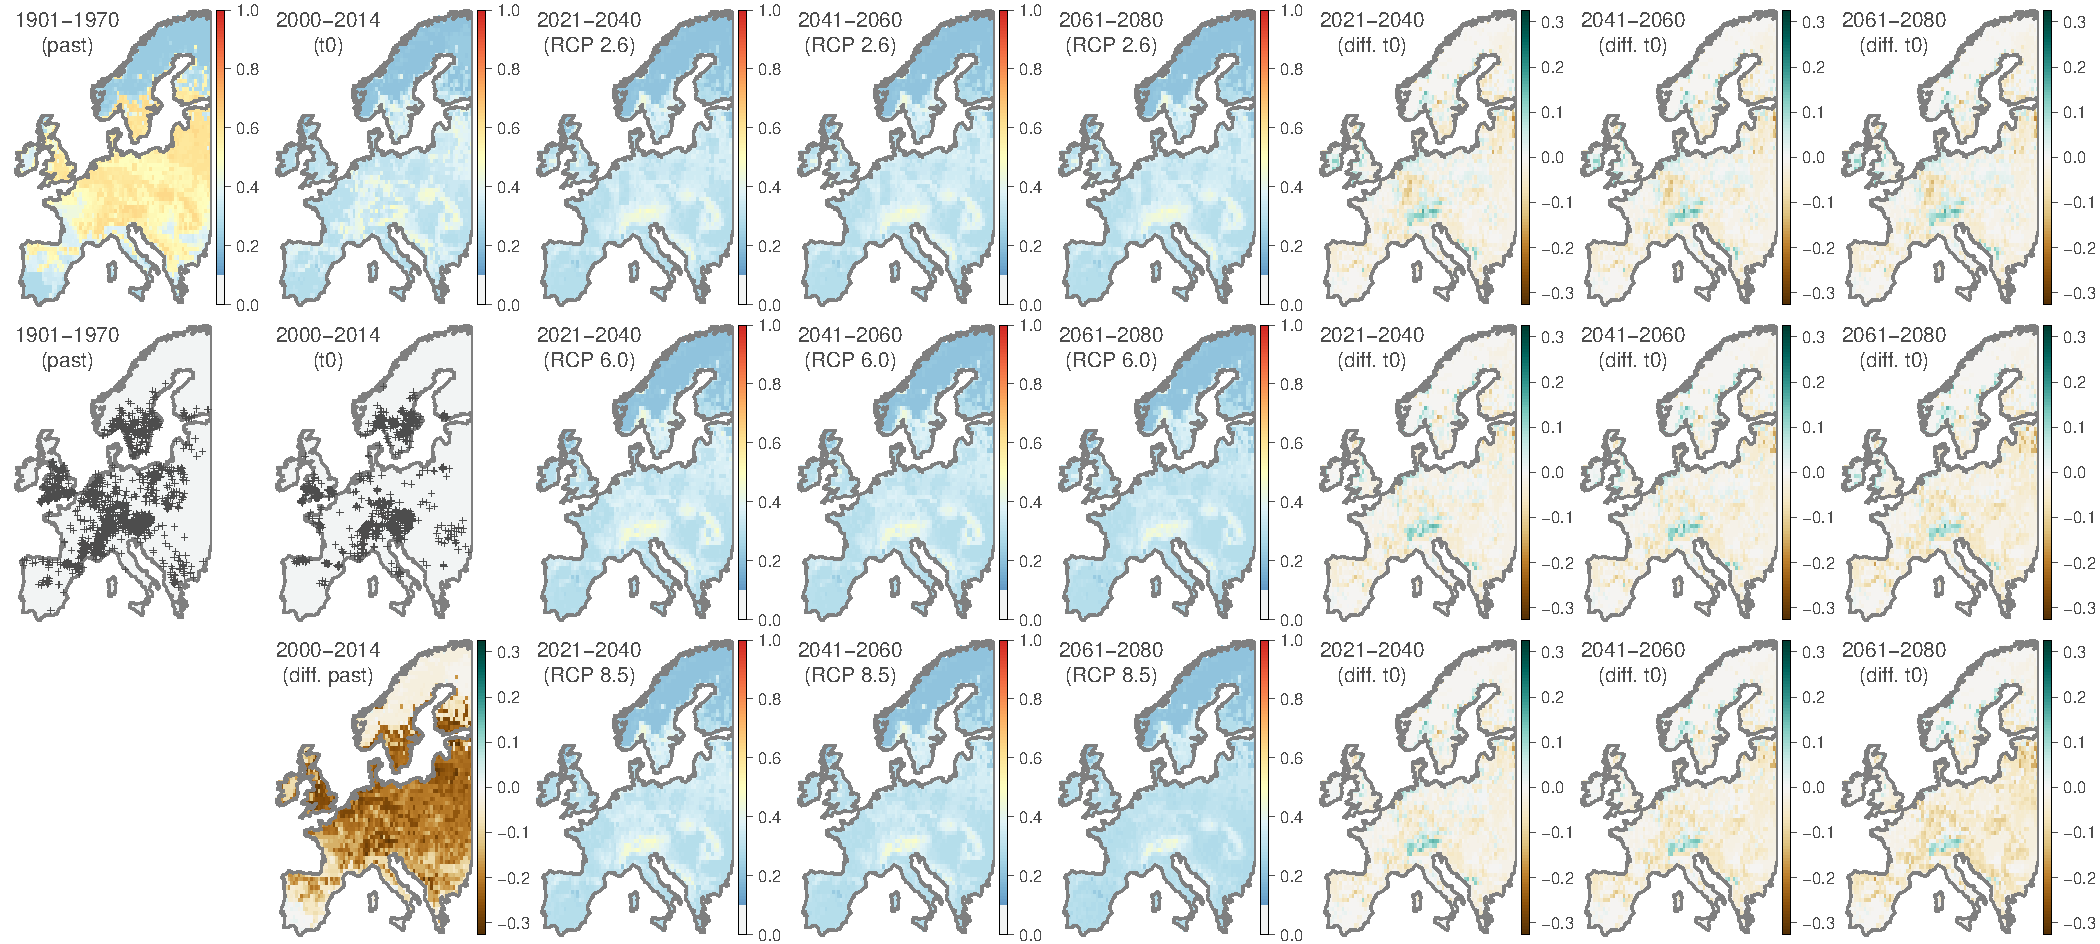
\includegraphics[width=1.00\textwidth]{All_the_species_projections/B_humilis_projections.pdf}}
\caption{\small{\textbf{Ecological niche modelling for \emph{Bombus humilis}.}
We report the projection for the current period as well as differences between future and current projections.}}
\label{FigureS25}
\end{figure}
\renewcommand{\thefigure}{S26}
\begin{figure}[H]
\centering
\makebox[\textwidth][c]{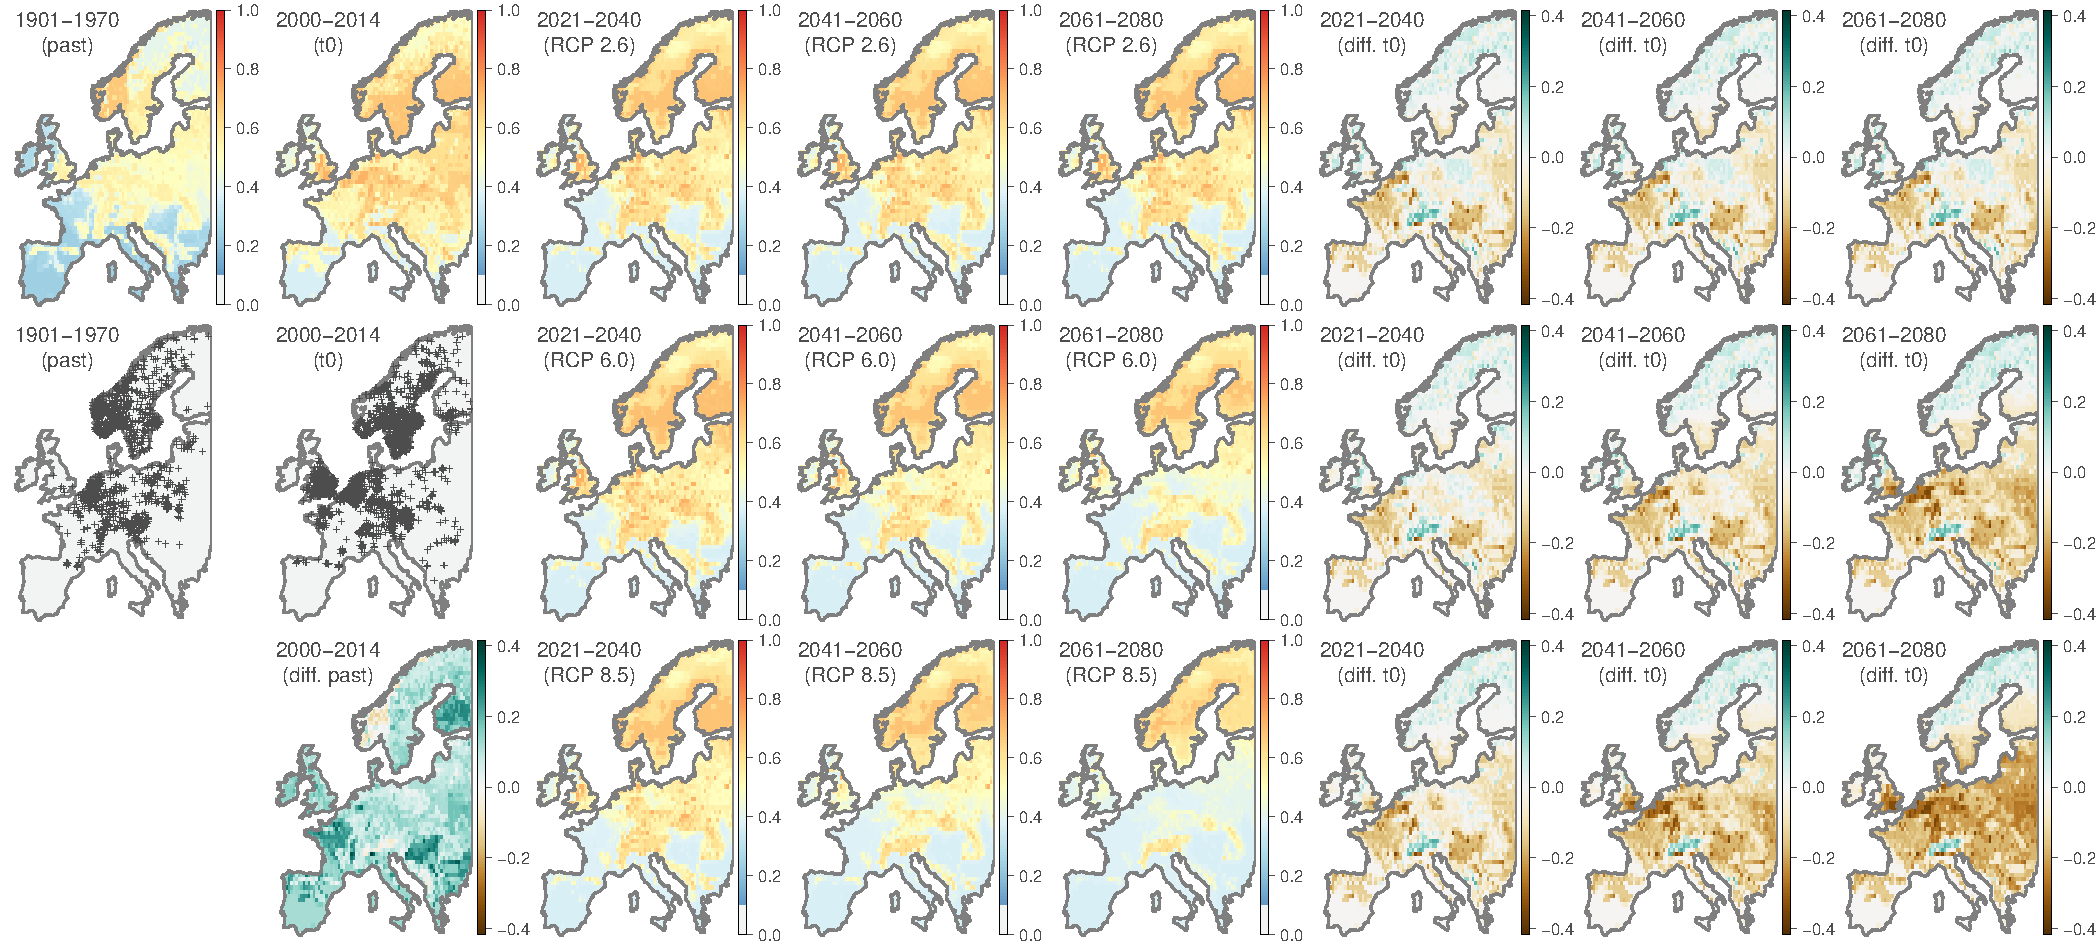
\includegraphics[width=1.00\textwidth]{All_the_species_projections/B_hypnorum_projections.pdf}}
\caption{\small{\textbf{Ecological niche modelling for \emph{Bombus hypnorum}.}
We report the projection for the current period as well as differences between future and current projections.}}
\label{FigureS26}
\end{figure}
\renewcommand{\thefigure}{S27}
\begin{figure}[H]
\centering
\makebox[\textwidth][c]{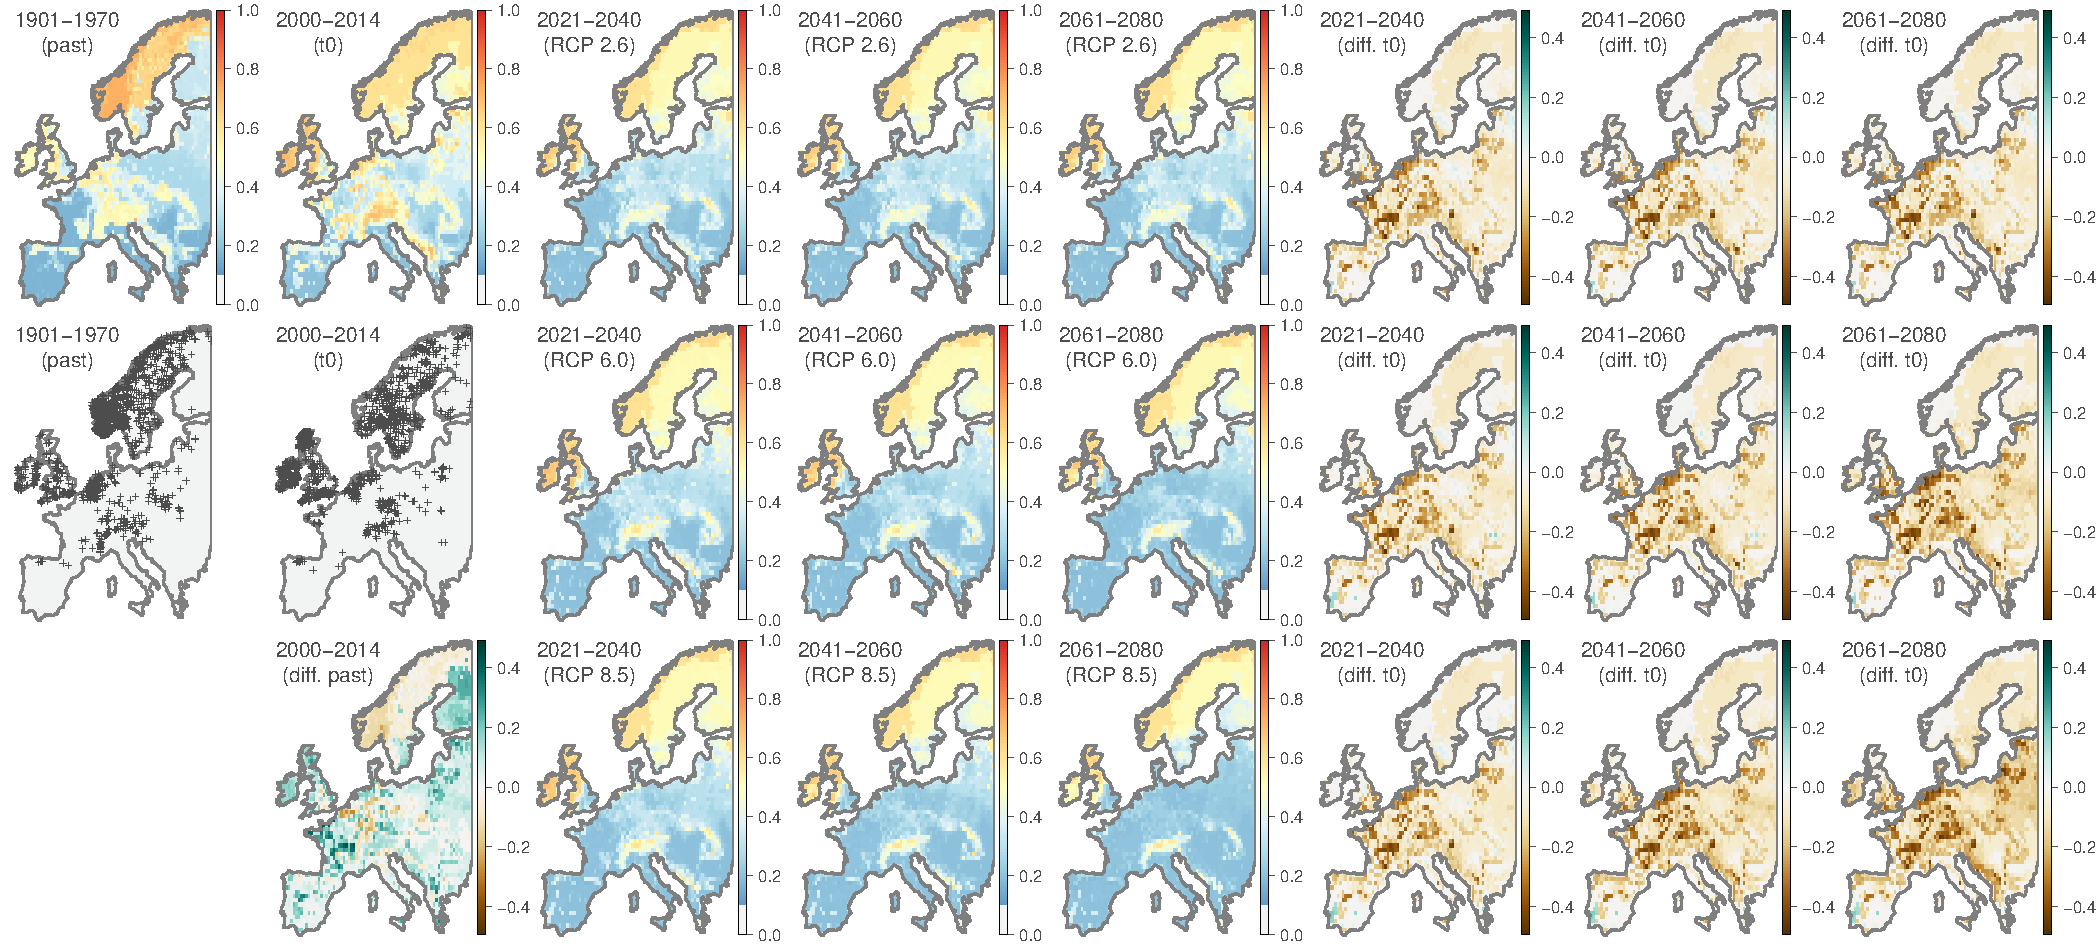
\includegraphics[width=1.00\textwidth]{All_the_species_projections/B_jonellus_projections.pdf}}
\caption{\small{\textbf{Ecological niche modelling for \emph{Bombus jonellus}.}
We report the projection for the current period as well as differences between future and current projections.}}
\label{FigureS27}
\end{figure}
\renewcommand{\thefigure}{S28}
\begin{figure}[H]
\centering
\makebox[\textwidth][c]{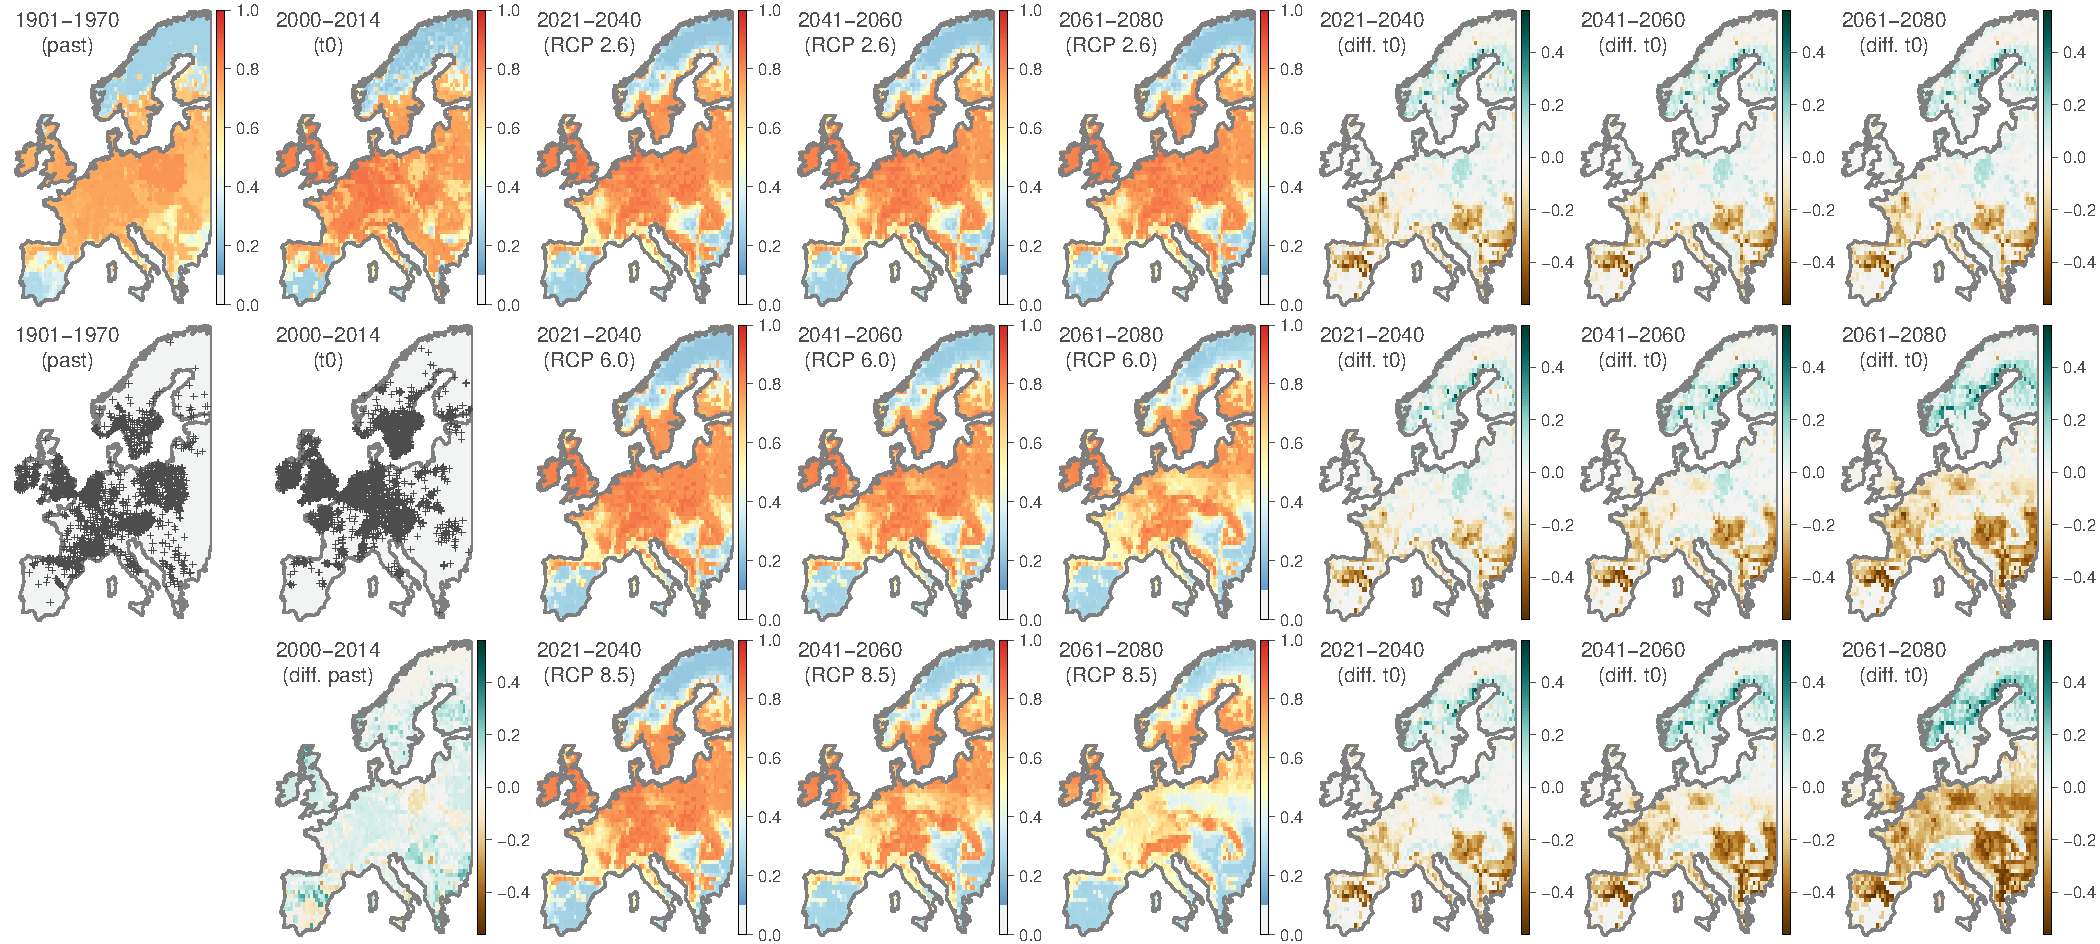
\includegraphics[width=1.00\textwidth]{All_the_species_projections/B_lapidarius_projections.pdf}}
\caption{\small{\textbf{Ecological niche modelling for \emph{Bombus lapidarius}.}
We report the projection for the current period as well as differences between future and current projections.}}
\label{FigureS28}
\end{figure}
\renewcommand{\thefigure}{S29}
\begin{figure}[H]
\centering
\makebox[\textwidth][c]{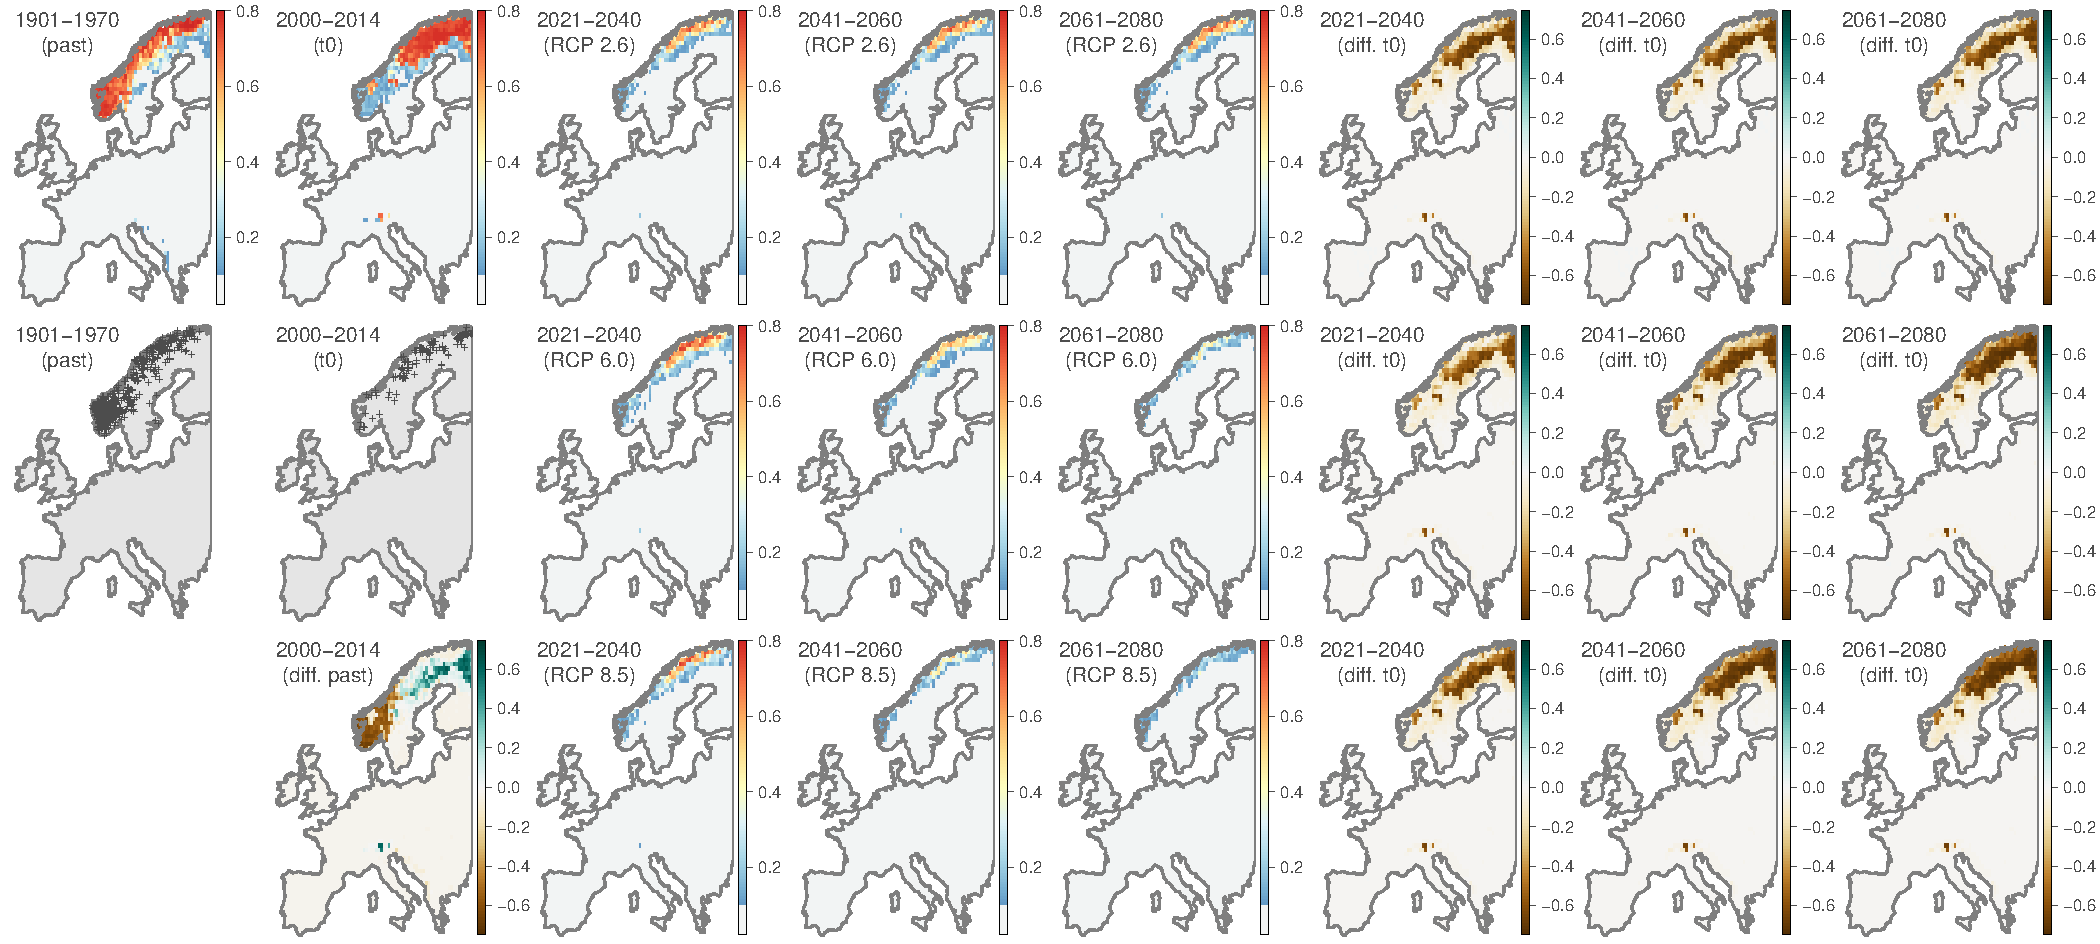
\includegraphics[width=1.00\textwidth]{All_the_species_projections/B_lapponicus_projections.pdf}}
\caption{\small{\textbf{Ecological niche modelling for \emph{Bombus lapponicus}.}
We report the projection for the current period as well as differences between future and current projections.}}
\label{FigureS29}
\end{figure}
\renewcommand{\thefigure}{S30}
\begin{figure}[H]
\centering
\makebox[\textwidth][c]{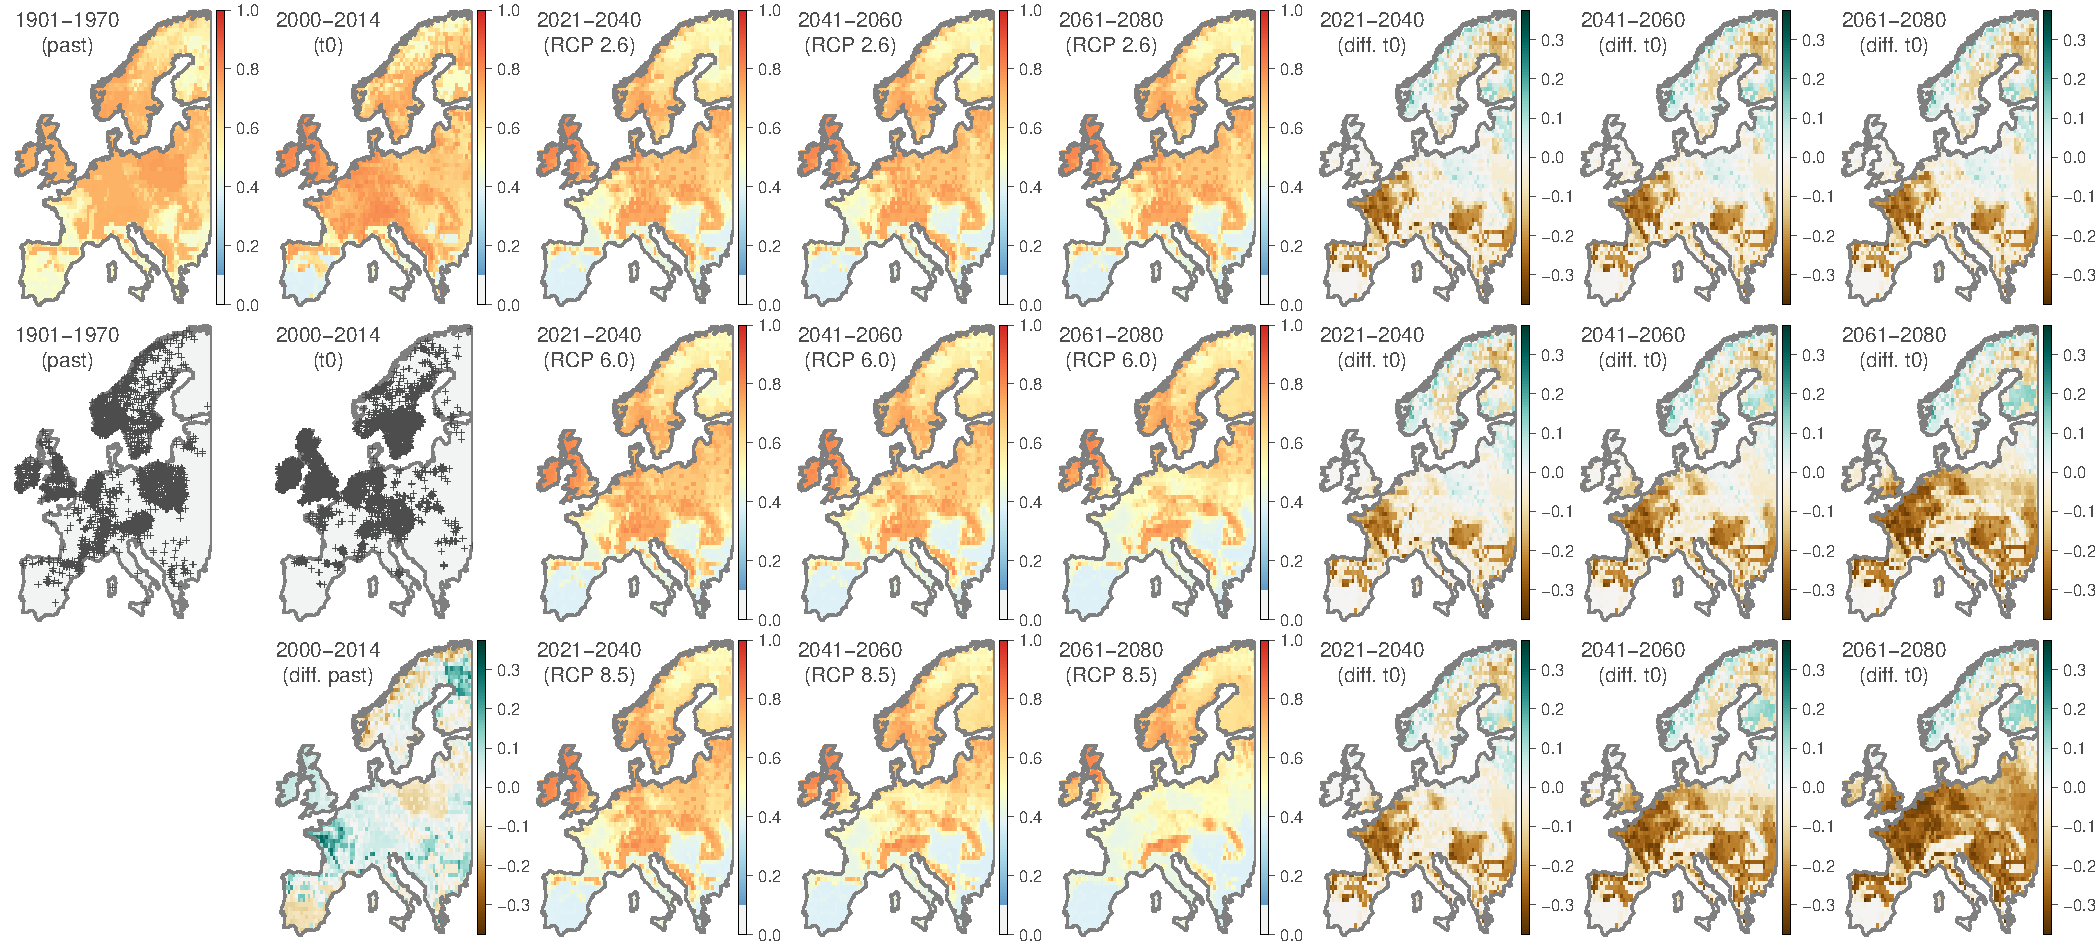
\includegraphics[width=1.00\textwidth]{All_the_species_projections/B_lucorum_projections.pdf}}
\caption{\small{\textbf{Ecological niche modelling for \emph{Bombus lucorum}.}
We report the projection for the current period as well as differences between future and current projections.}}
\label{FigureS30}
\end{figure}
\renewcommand{\thefigure}{S31}
\begin{figure}[H]
\centering
\makebox[\textwidth][c]{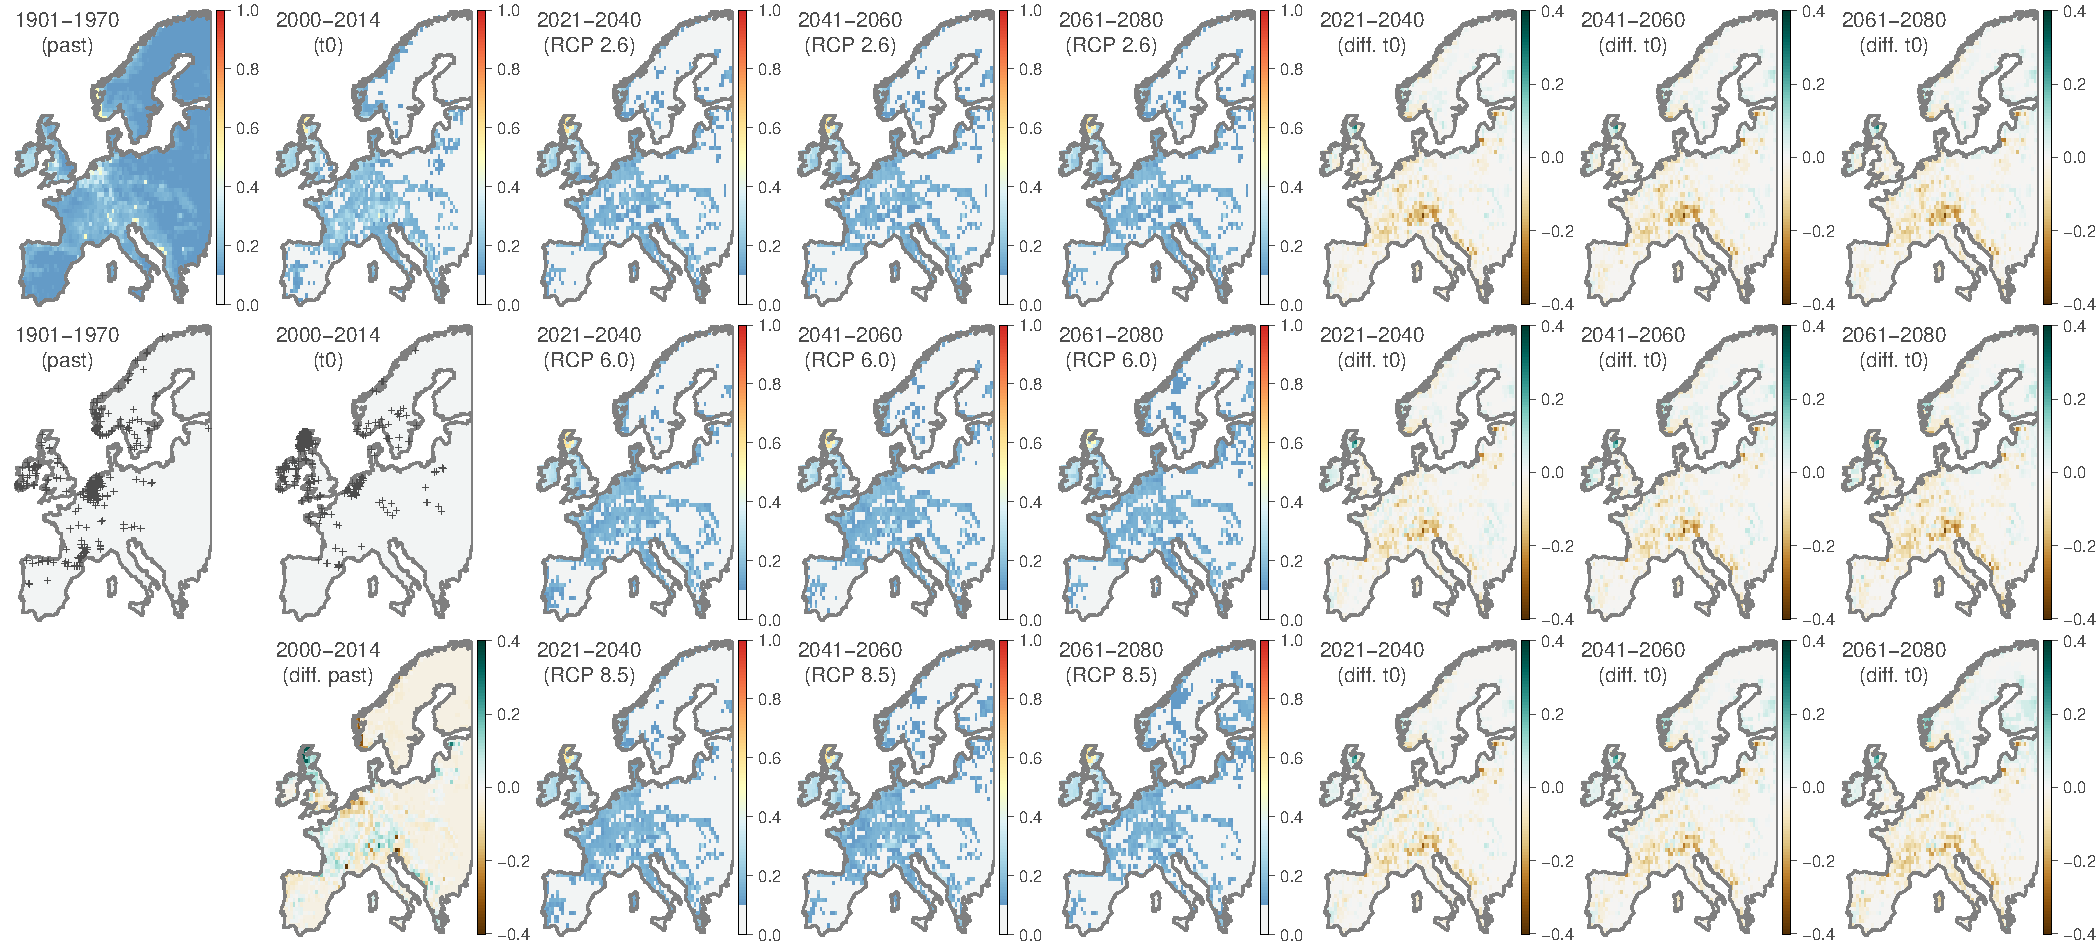
\includegraphics[width=1.00\textwidth]{All_the_species_projections/B_magnus_projections.pdf}}
\caption{\small{\textbf{Ecological niche modelling for \emph{Bombus magnus}.}
We report the projection for the current period as well as differences between future and current projections.}}
\label{FigureS31}
\end{figure}
\renewcommand{\thefigure}{S32}
\begin{figure}[H]
\centering
\makebox[\textwidth][c]{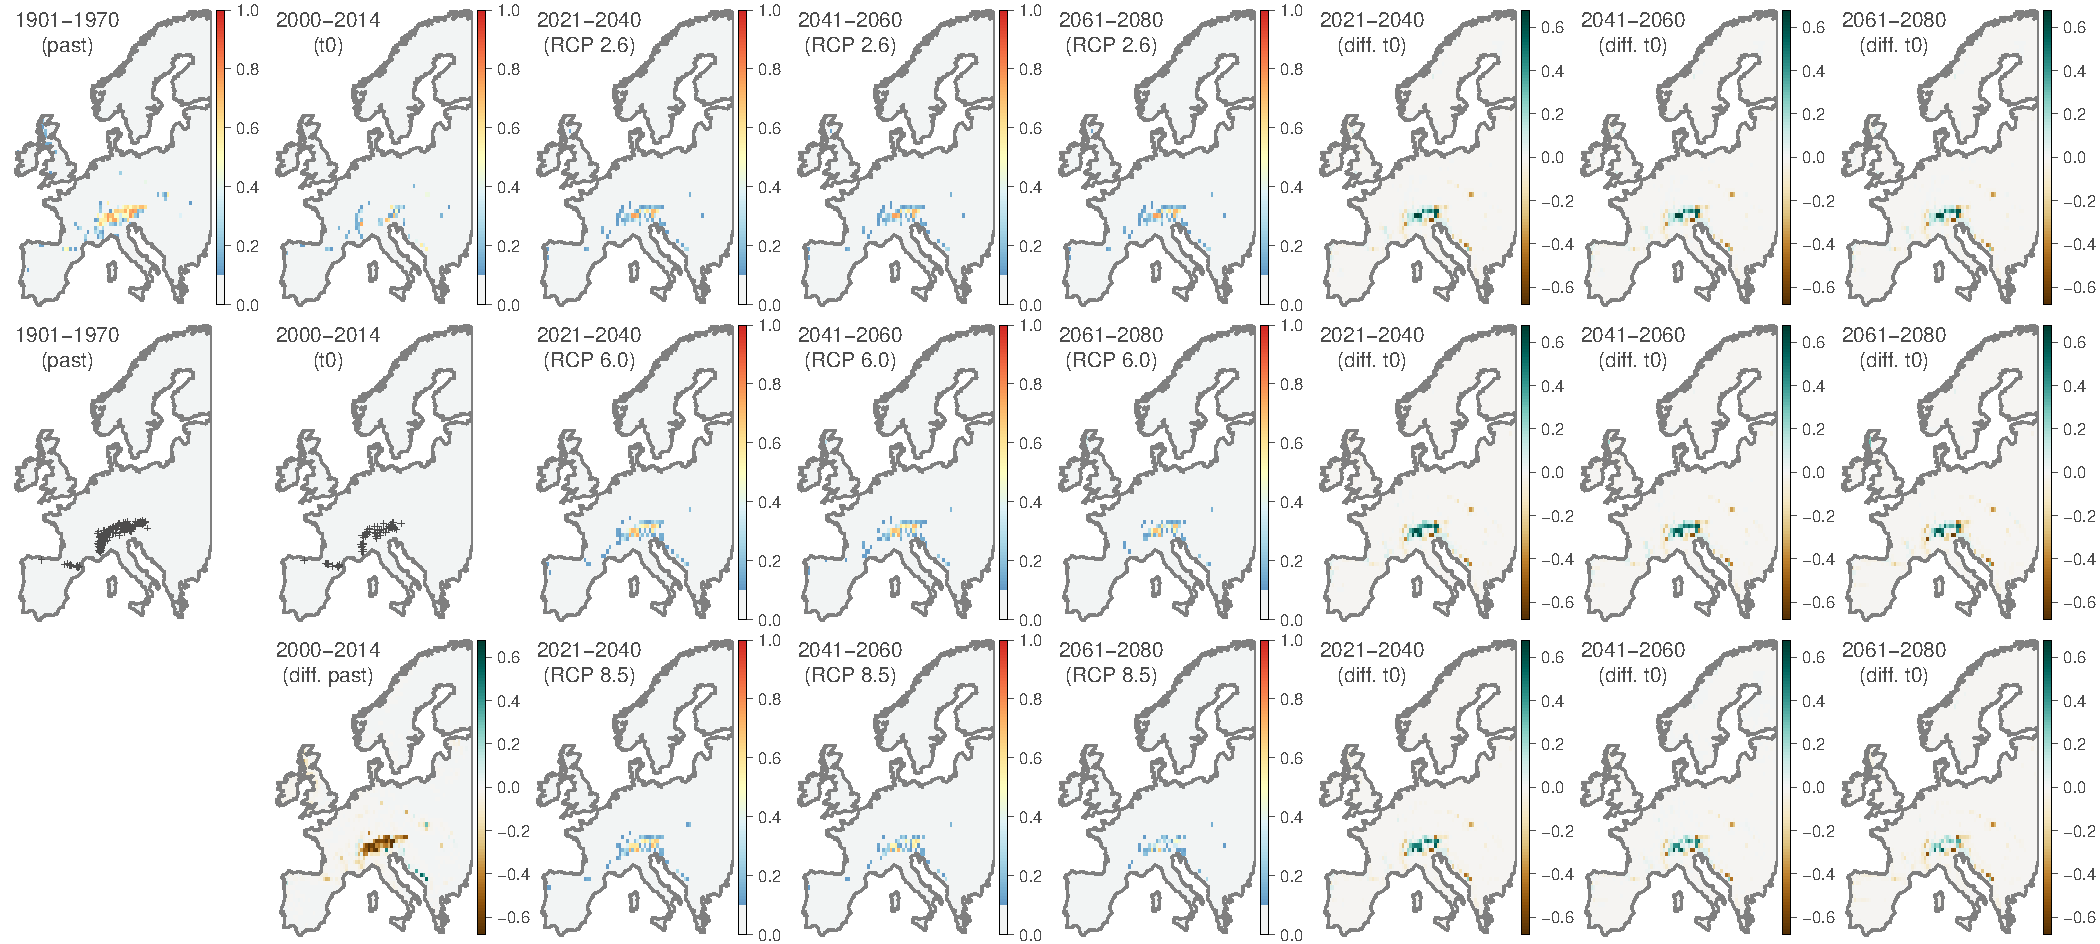
\includegraphics[width=1.00\textwidth]{All_the_species_projections/B_mendax_projections.pdf}}
\caption{\small{\textbf{Ecological niche modelling for \emph{Bombus mendax}.}
We report the projection for the current period as well as differences between future and current projections.}}
\label{FigureS32}
\end{figure}
\renewcommand{\thefigure}{S33}
\begin{figure}[H]
\centering
\makebox[\textwidth][c]{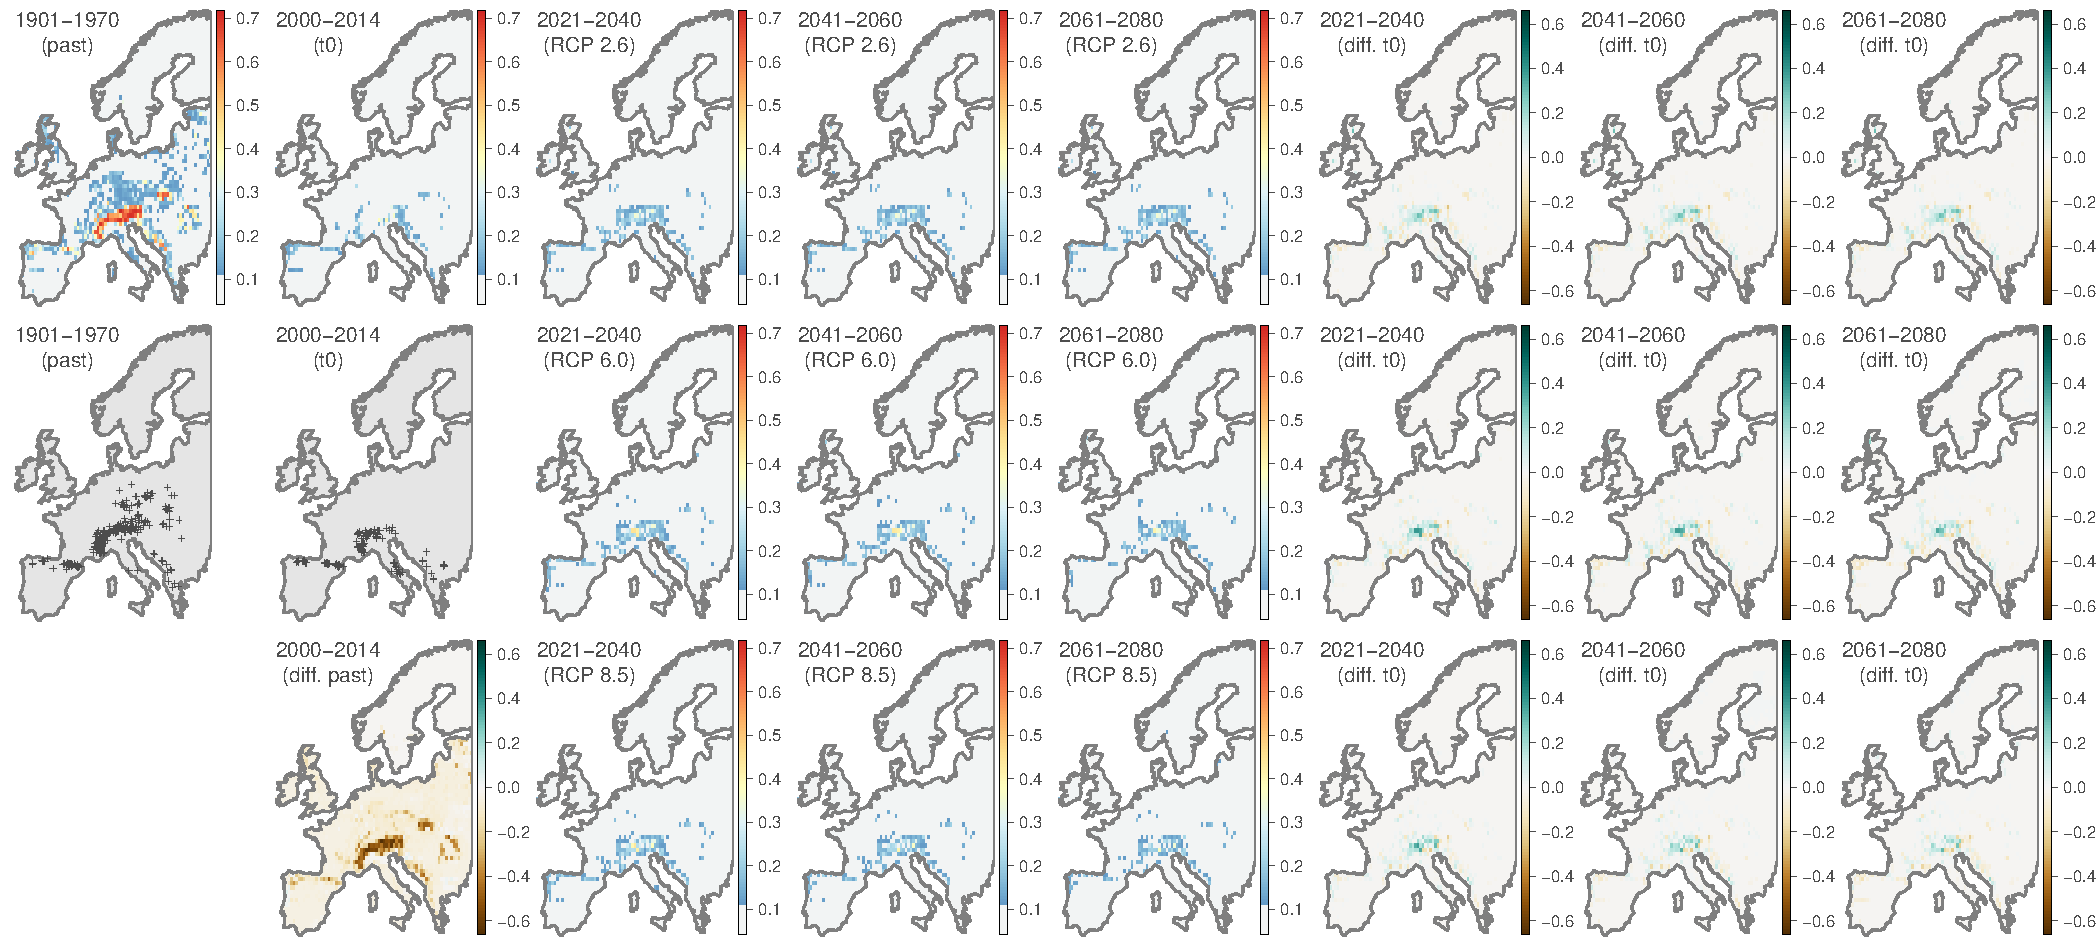
\includegraphics[width=1.00\textwidth]{All_the_species_projections/B_mesomelas_projections.pdf}}
\caption{\small{\textbf{Ecological niche modelling for \emph{Bombus mesomelas}.}
We report the projection for the current period as well as differences between future and current projections.}}
\label{FigureS33}
\end{figure}
\renewcommand{\thefigure}{S34}
\begin{figure}[H]
\centering
\makebox[\textwidth][c]{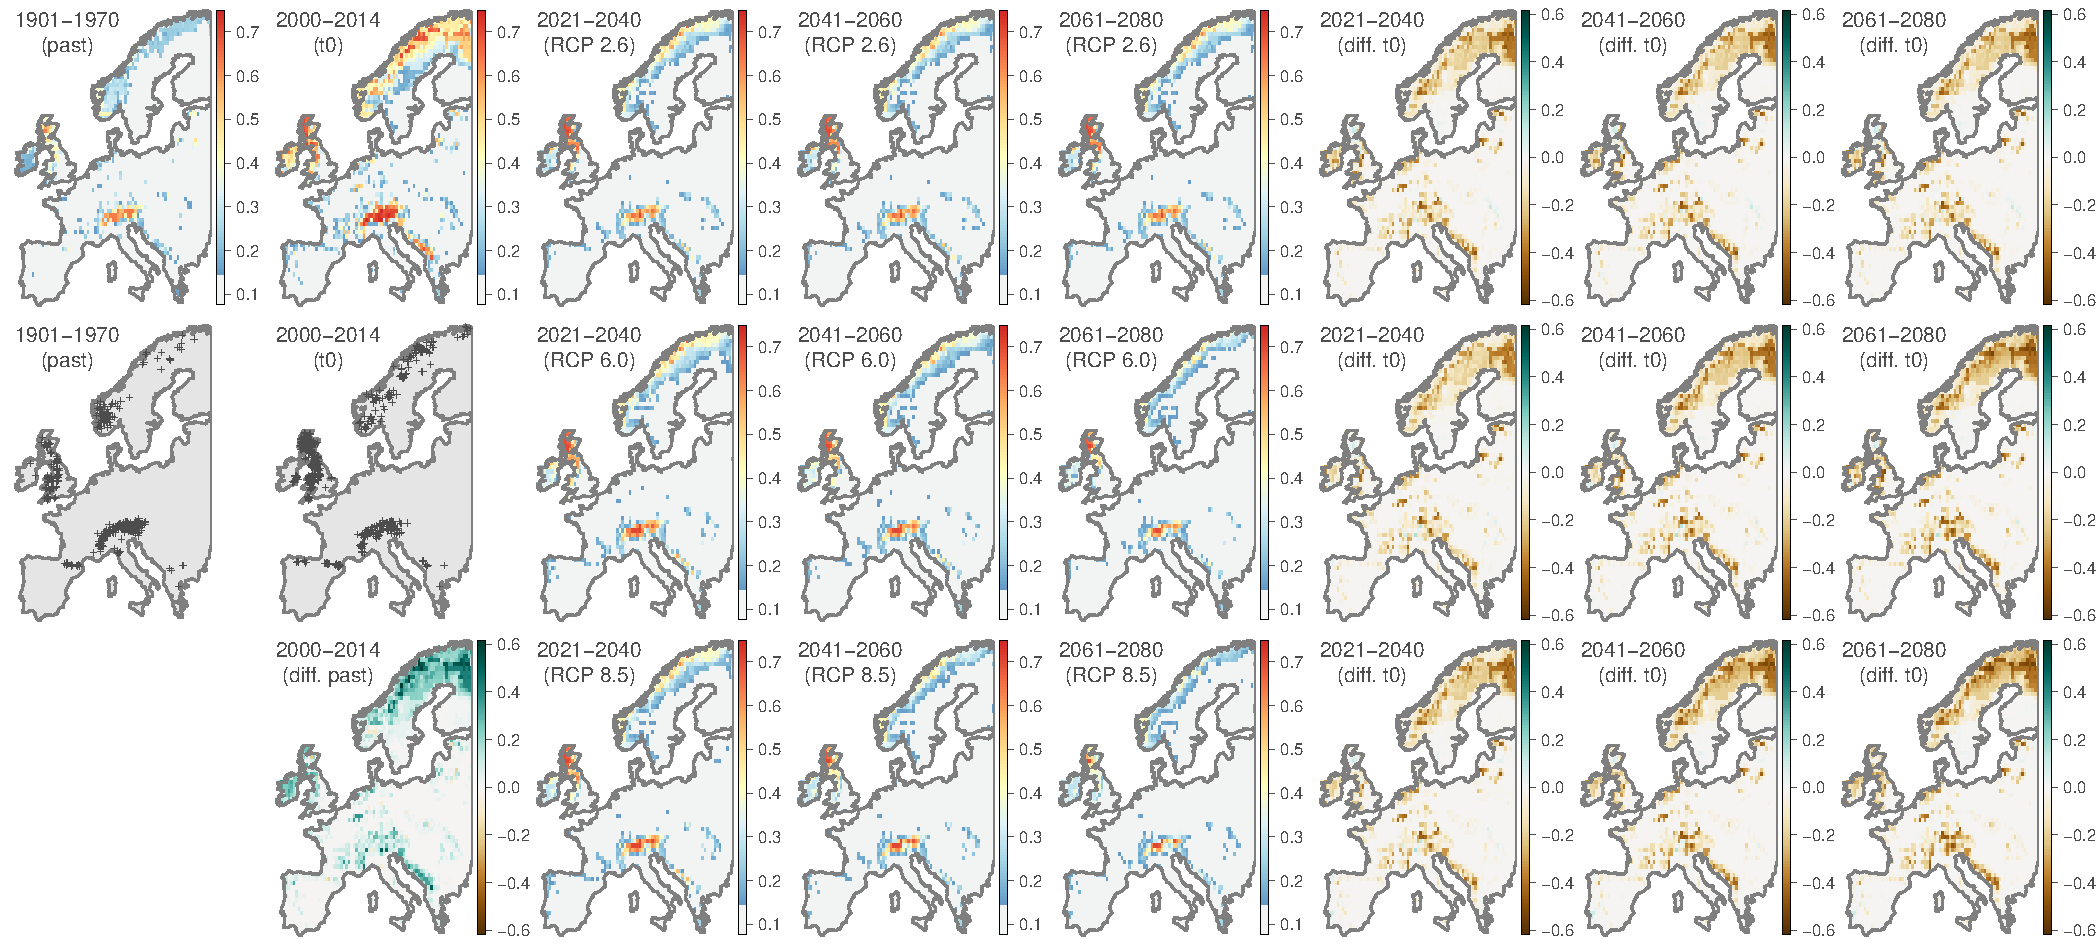
\includegraphics[width=1.00\textwidth]{All_the_species_projections/B_monticola_projections.pdf}}
\caption{\small{\textbf{Ecological niche modelling for \emph{Bombus monticola}.}
We report the projection for the current period as well as differences between future and current projections.}}
\label{FigureS34}
\end{figure}
\renewcommand{\thefigure}{S35}
\begin{figure}[H]
\centering
\makebox[\textwidth][c]{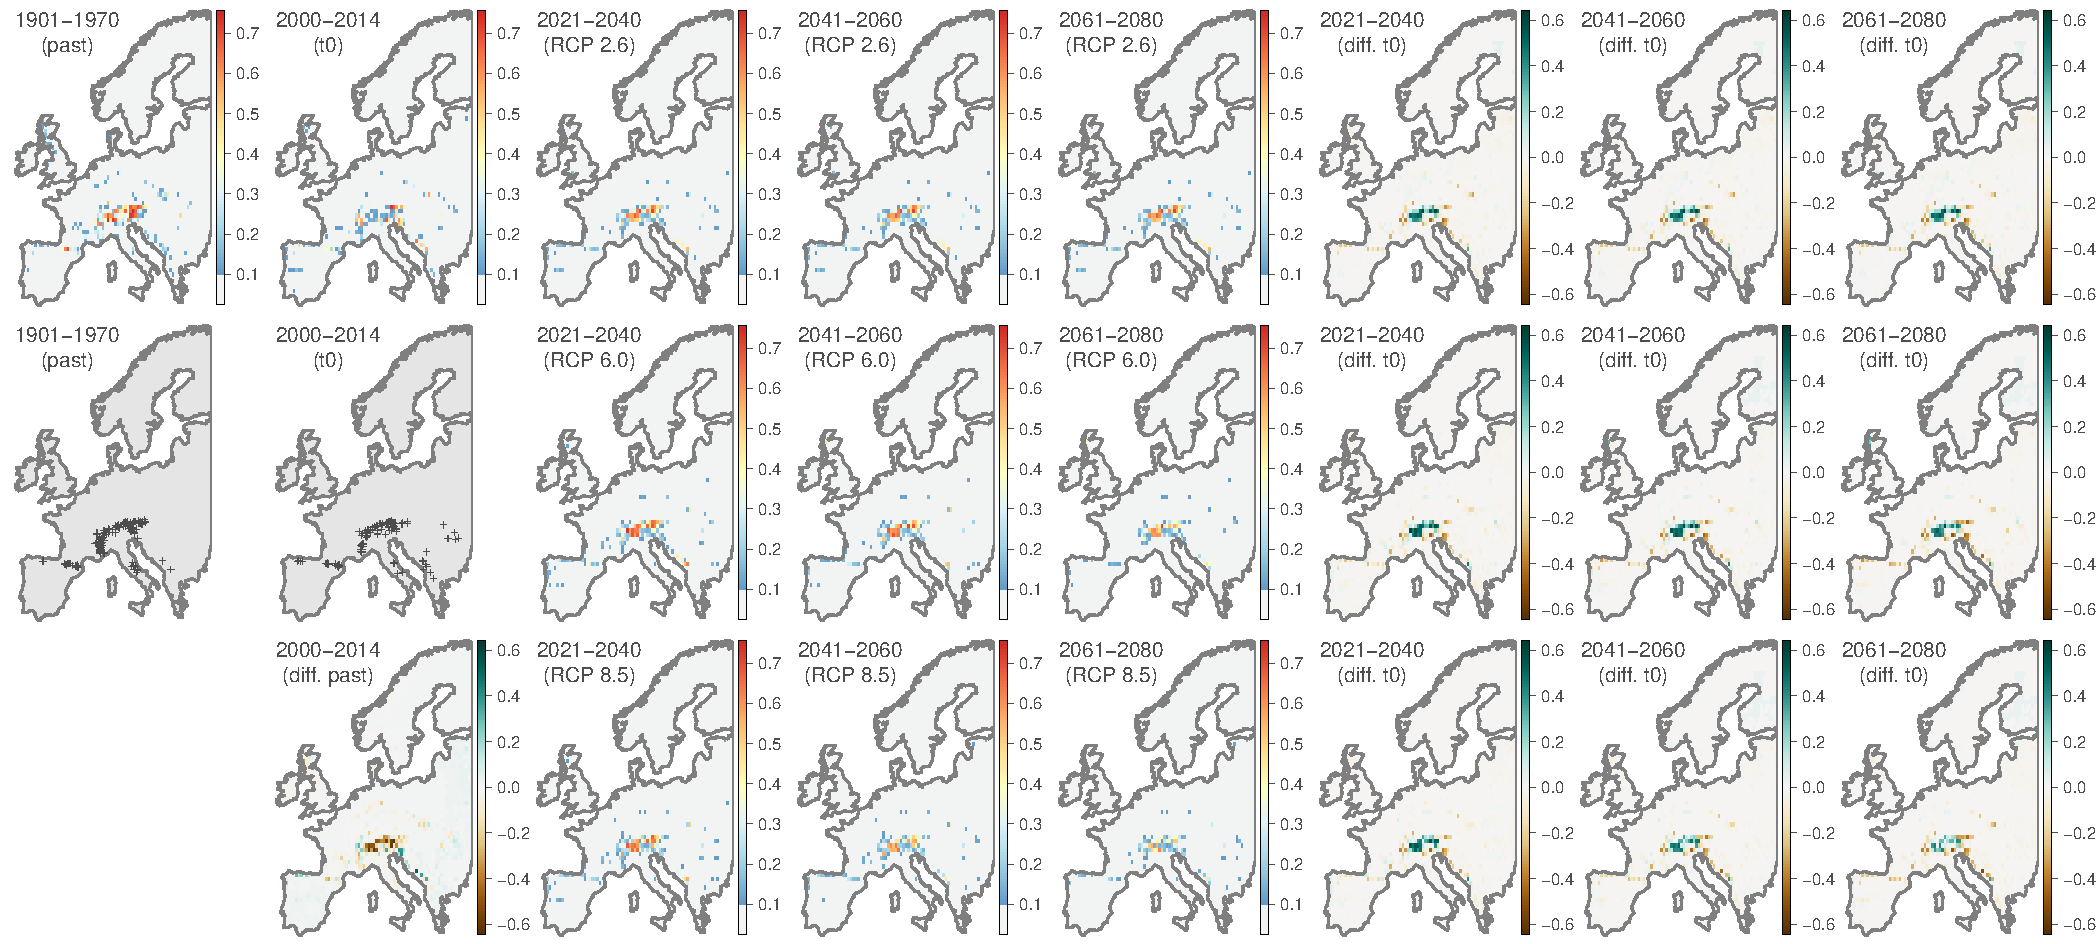
\includegraphics[width=1.00\textwidth]{All_the_species_projections/B_mucidus_projections.pdf}}
\caption{\small{\textbf{Ecological niche modelling for \emph{Bombus mucidus}.}
We report the projection for the current period as well as differences between future and current projections.}}
\label{FigureS35}
\end{figure}
\renewcommand{\thefigure}{S36}
\begin{figure}[H]
\centering
\makebox[\textwidth][c]{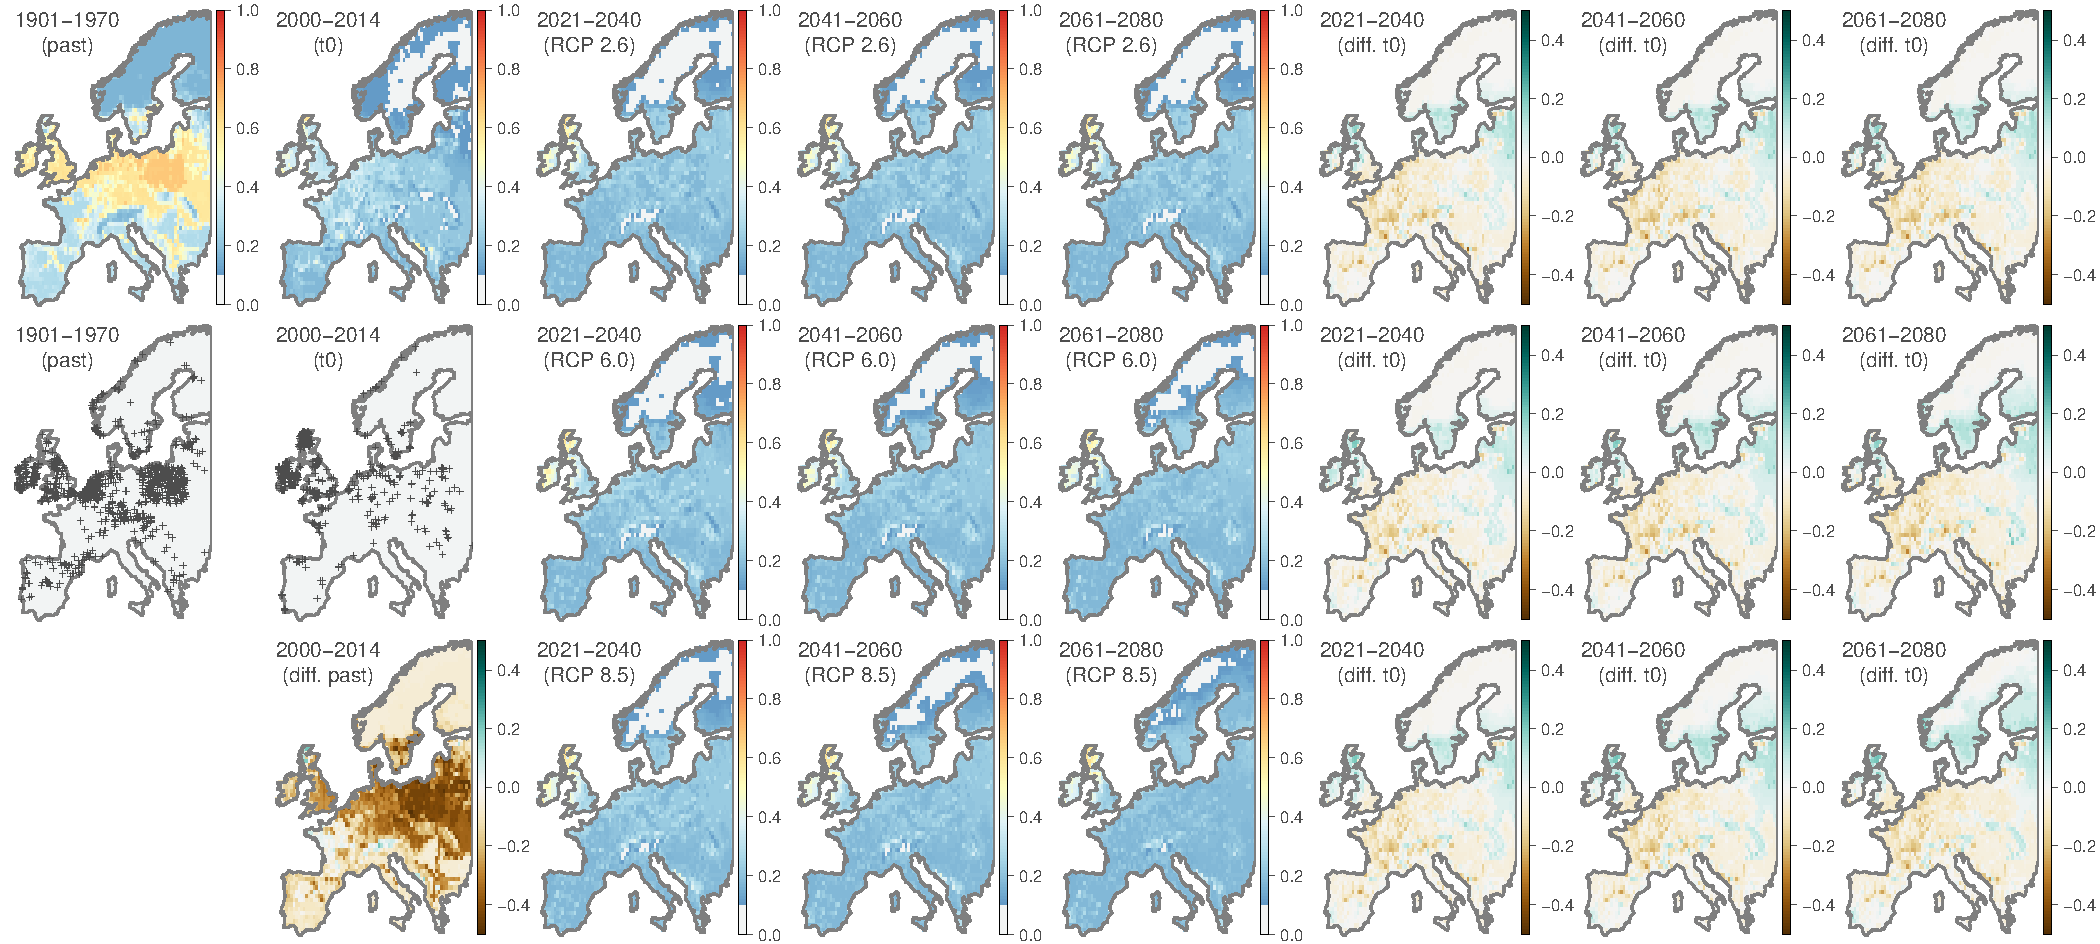
\includegraphics[width=1.00\textwidth]{All_the_species_projections/B_muscorum_projections.pdf}}
\caption{\small{\textbf{Ecological niche modelling for \emph{Bombus muscorum}.}
We report the projection for the current period as well as differences between future and current projections.}}
\label{FigureS36}
\end{figure}
\renewcommand{\thefigure}{S37}
\begin{figure}[H]
\centering
\makebox[\textwidth][c]{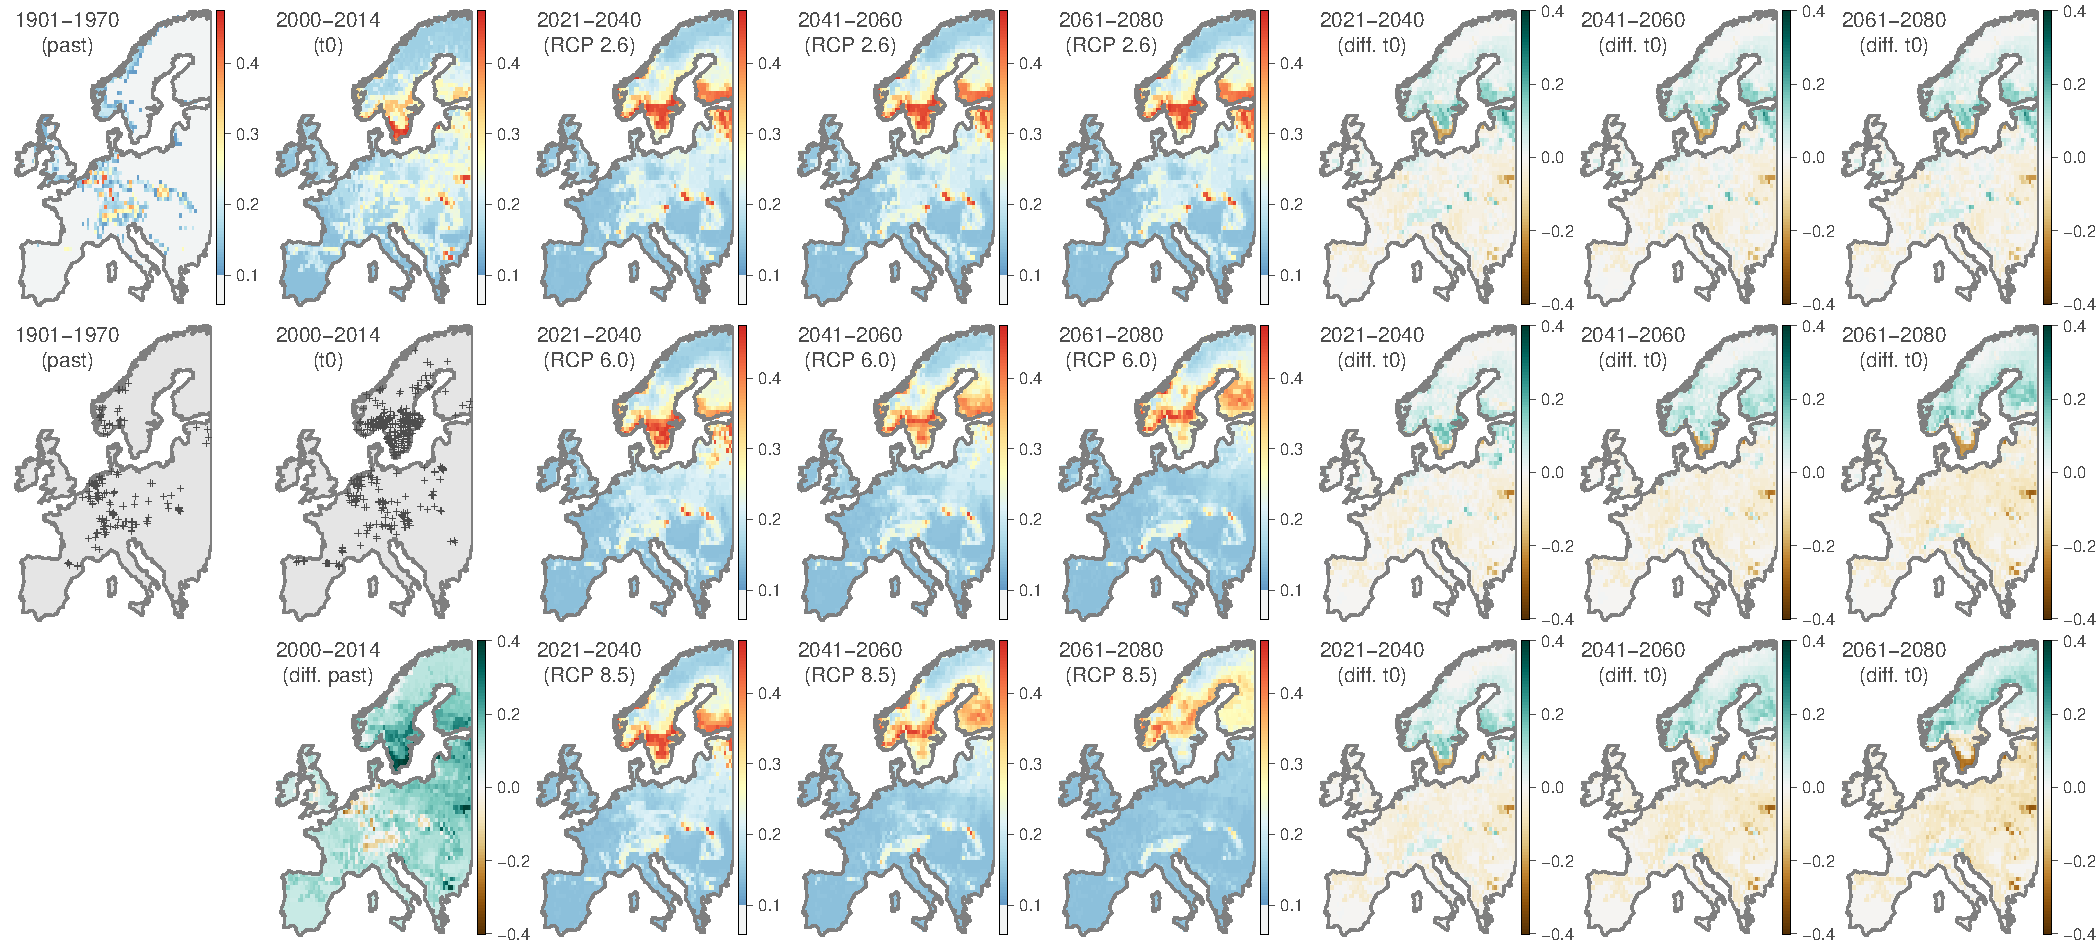
\includegraphics[width=1.00\textwidth]{All_the_species_projections/B_norvegicus_projections.pdf}}
\caption{\small{\textbf{Ecological niche modelling for \emph{Bombus norvegicus}.}
We report the projection for the current period as well as differences between future and current projections.}}
\label{FigureS37}
\end{figure}
\renewcommand{\thefigure}{S38}
\begin{figure}[H]
\centering
\makebox[\textwidth][c]{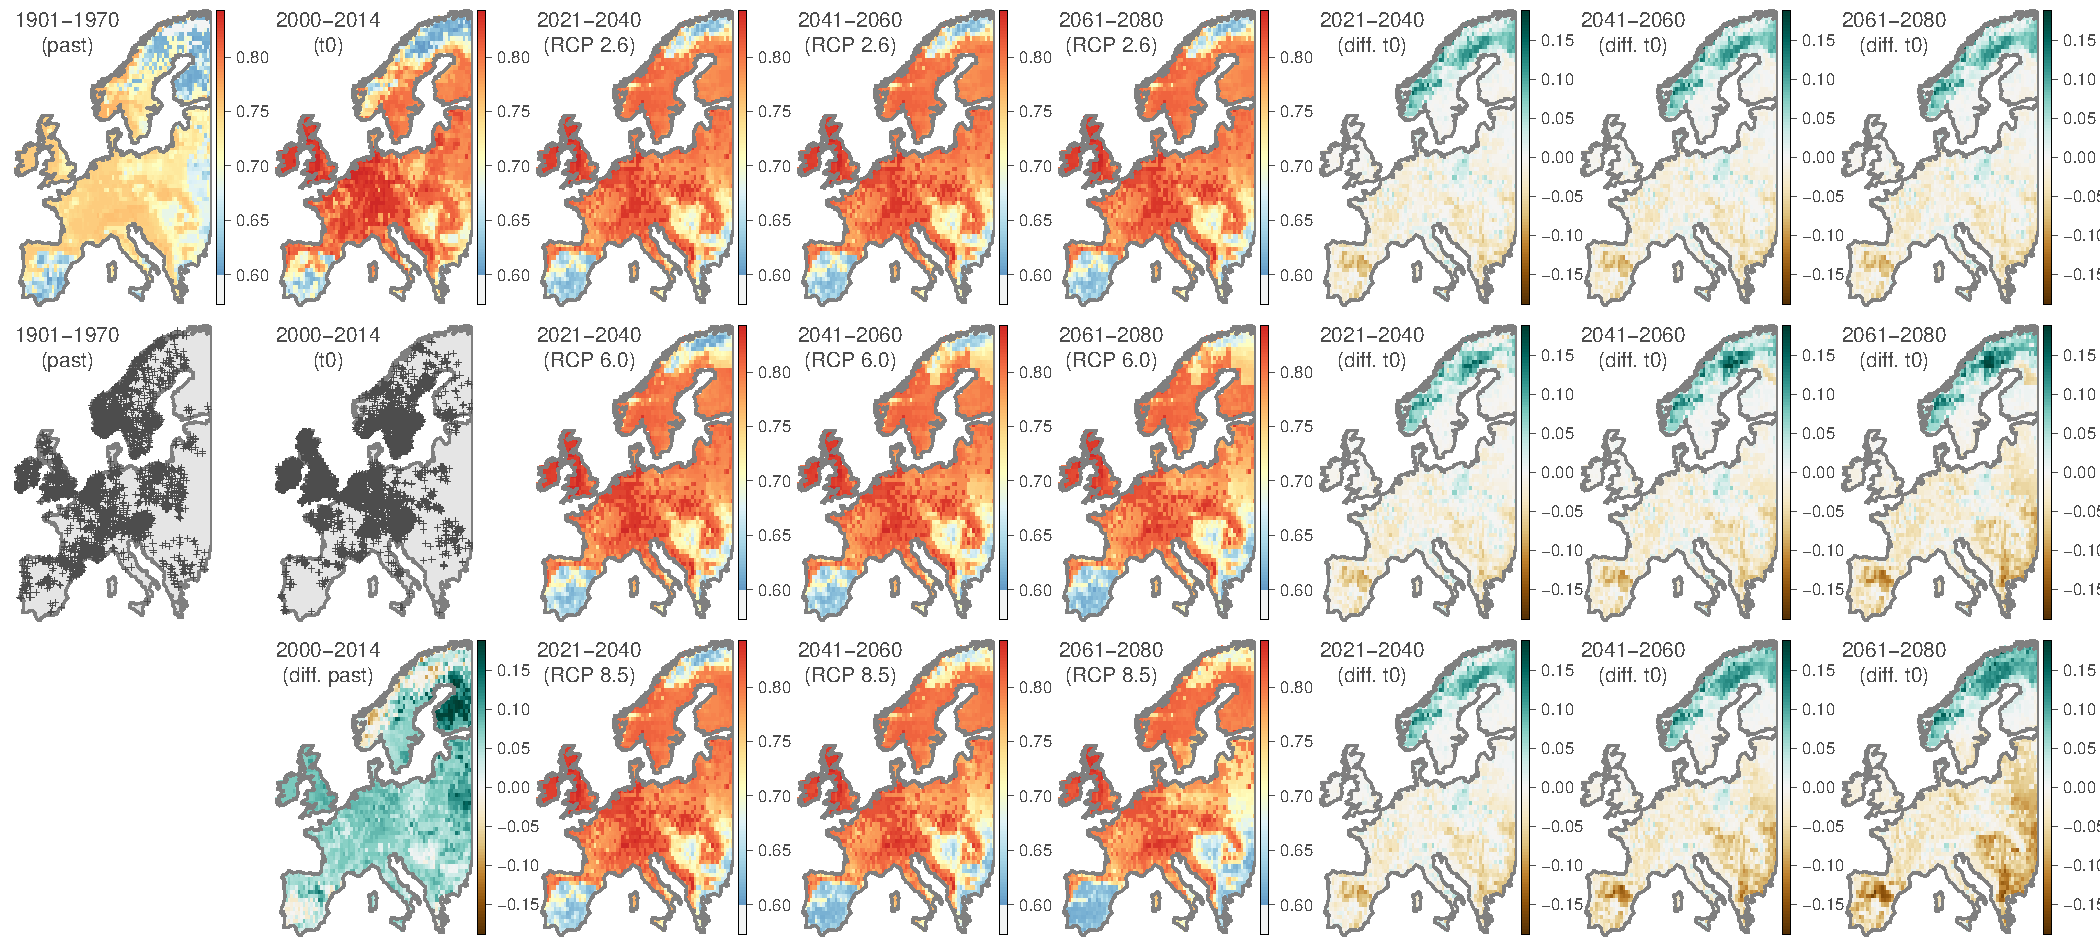
\includegraphics[width=1.00\textwidth]{All_the_species_projections/B_pascuorum_projections.pdf}}
\caption{\small{\textbf{Ecological niche modelling for \emph{Bombus pascuorum}.}
We report the projection for the current period as well as differences between future and current projections.}}
\label{FigureS38}
\end{figure}
\renewcommand{\thefigure}{S39}
\begin{figure}[H]
\centering
\makebox[\textwidth][c]{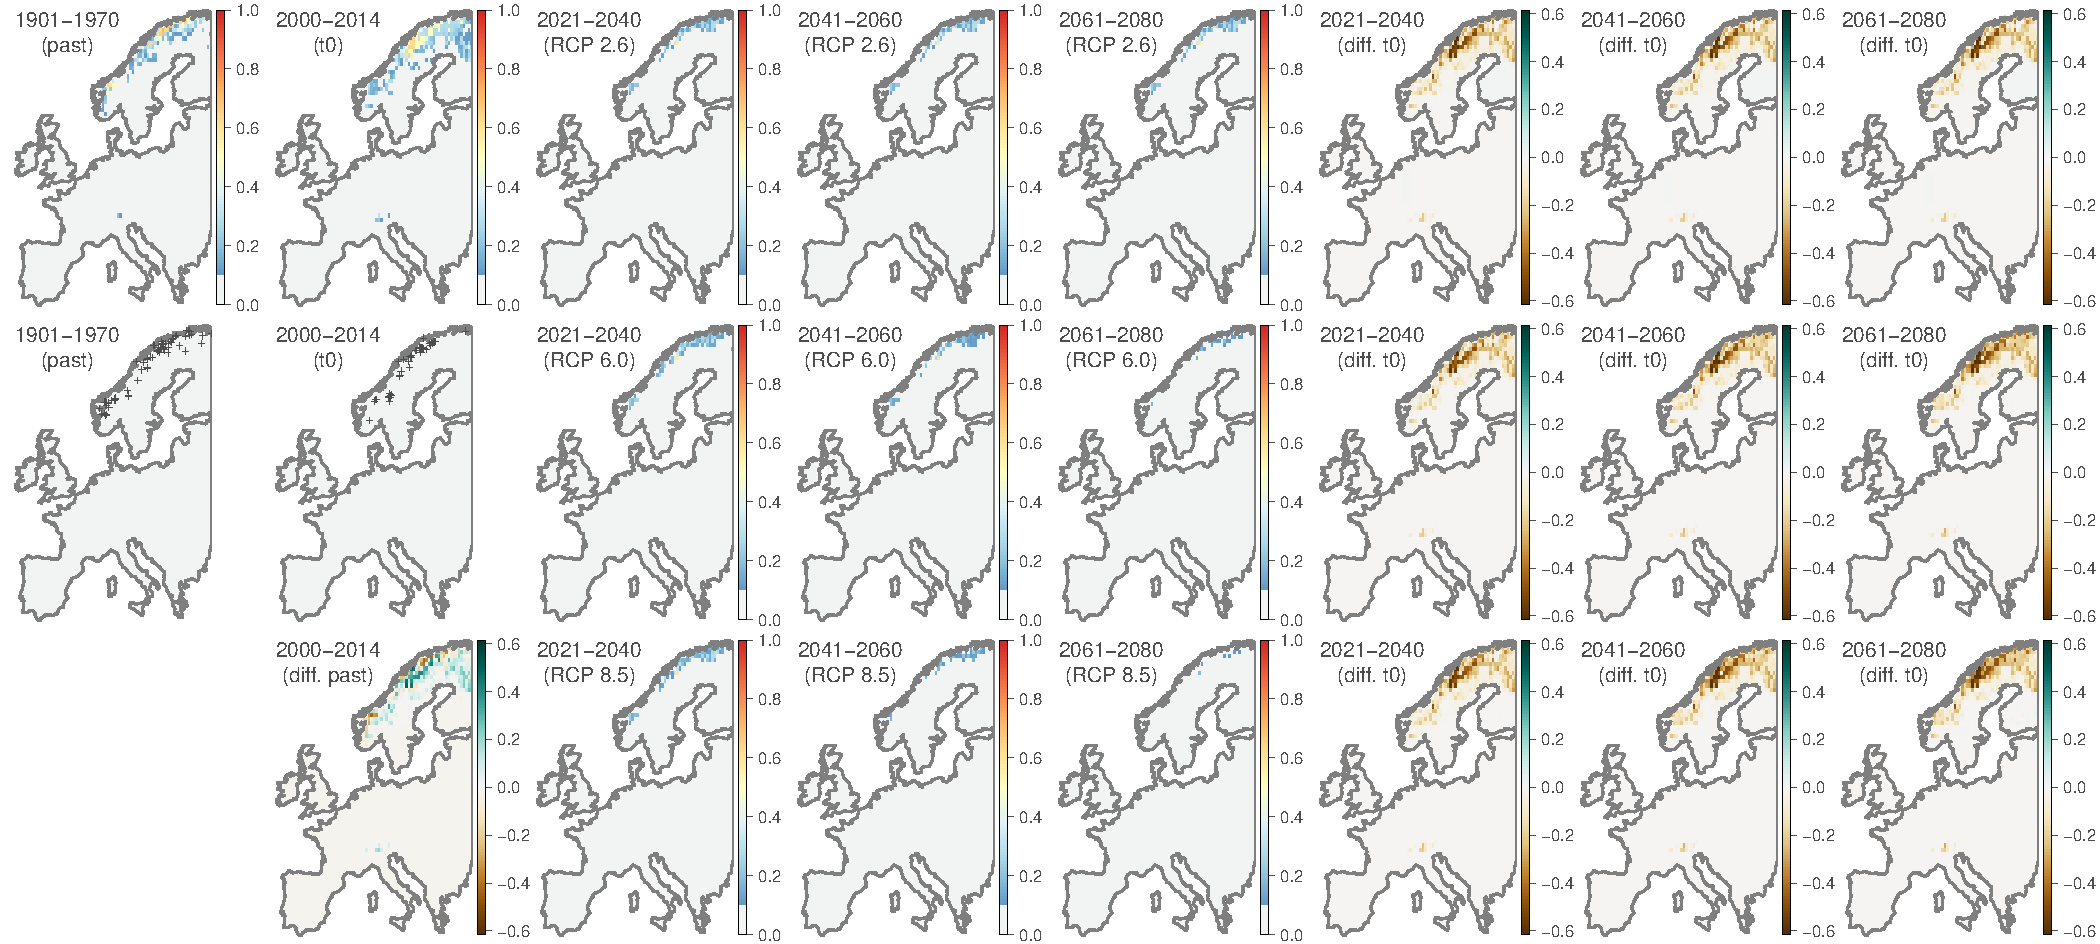
\includegraphics[width=1.00\textwidth]{All_the_species_projections/B_polaris_projections.pdf}}
\caption{\small{\textbf{Ecological niche modelling for \emph{Bombus polaris}.}
We report the projection for the current period as well as differences between future and current projections.}}
\label{FigureS39}
\end{figure}
\renewcommand{\thefigure}{S40}
\begin{figure}[H]
\centering
\makebox[\textwidth][c]{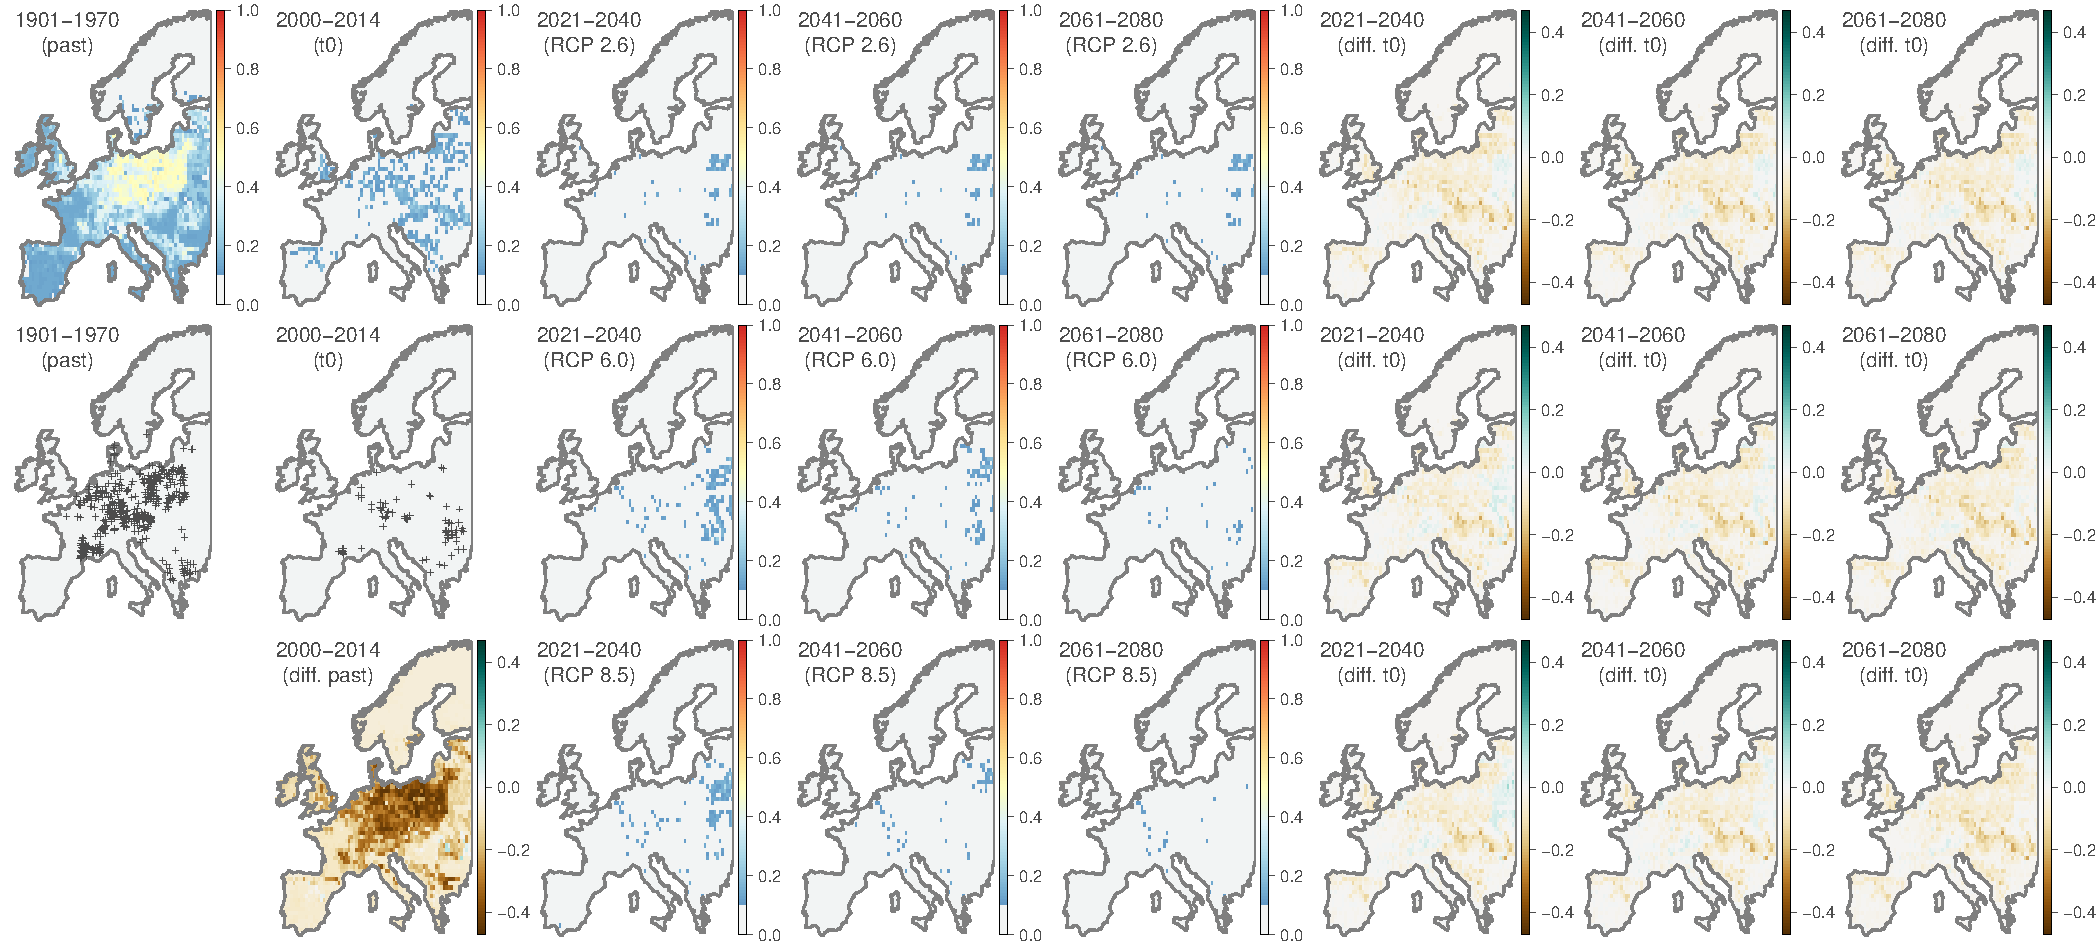
\includegraphics[width=1.00\textwidth]{All_the_species_projections/B_pomorum_projections.pdf}}
\caption{\small{\textbf{Ecological niche modelling for \emph{Bombus pomorum}.}
We report the projection for the current period as well as differences between future and current projections.}}
\label{FigureS40}
\end{figure}
\renewcommand{\thefigure}{S41}
\begin{figure}[H]
\centering
\makebox[\textwidth][c]{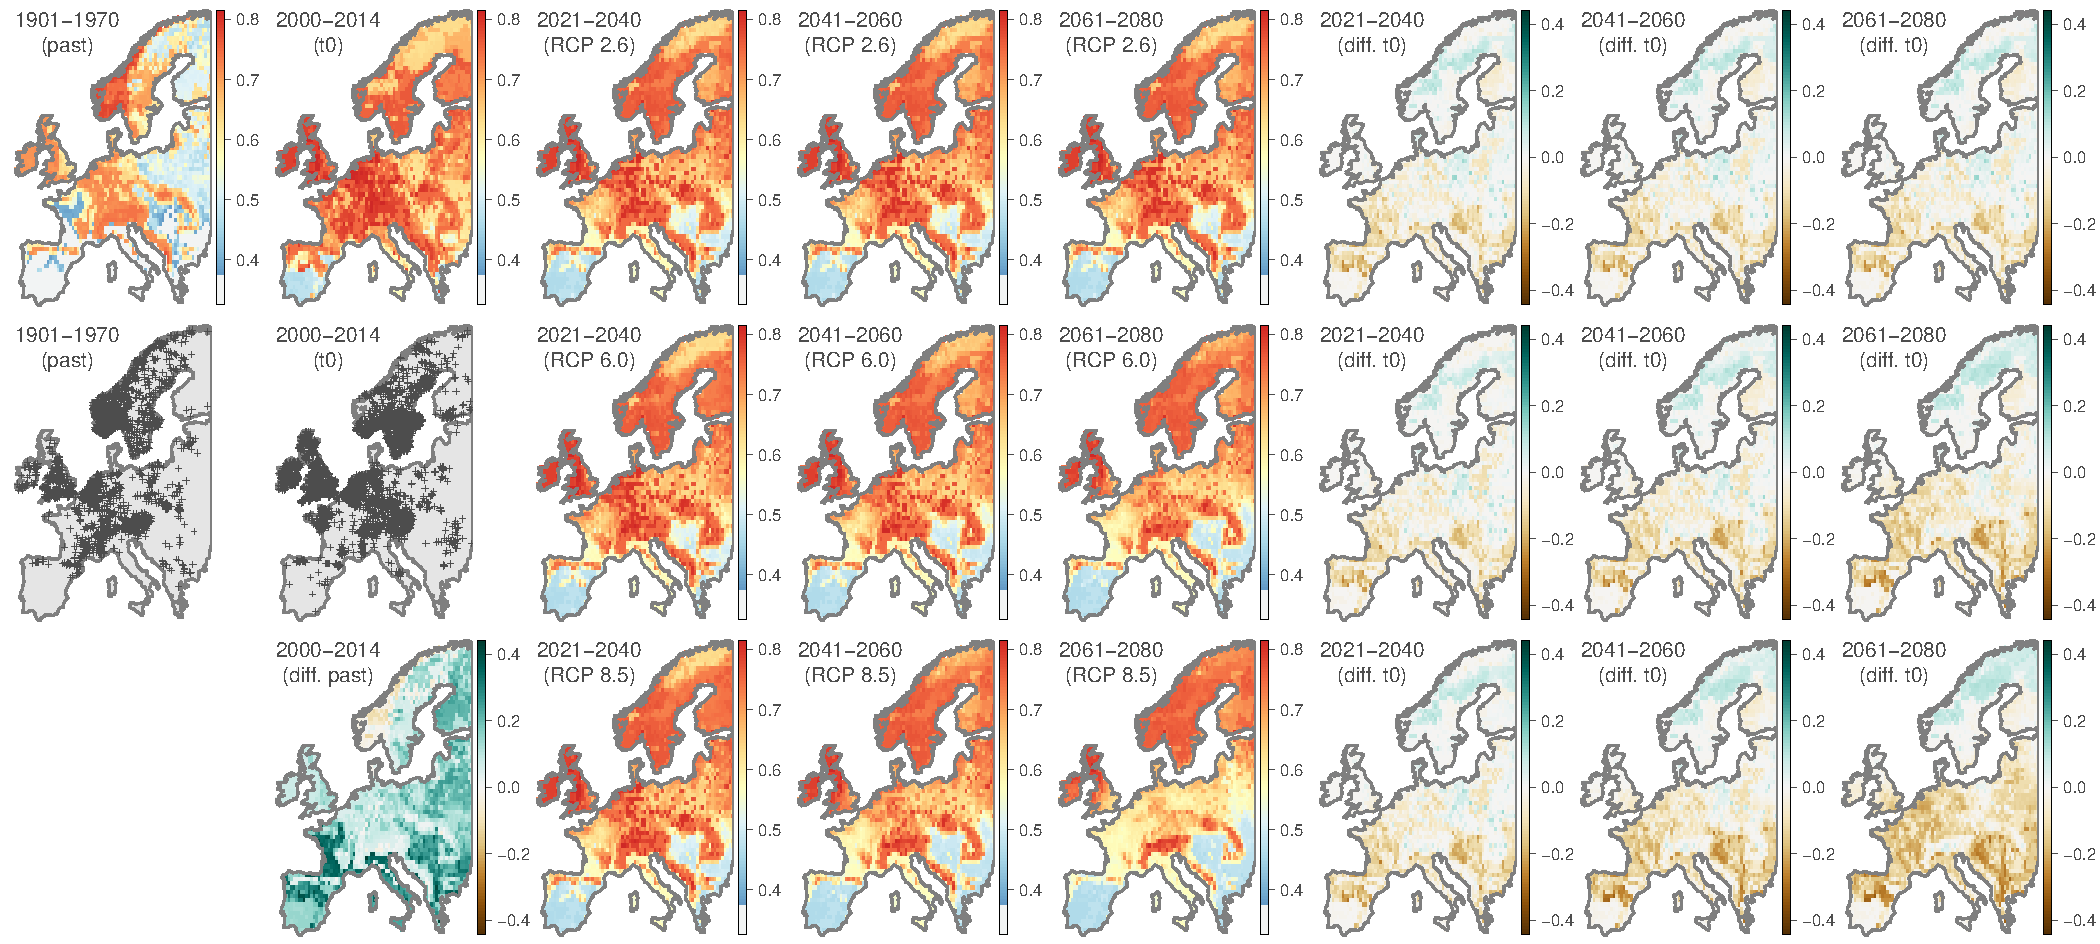
\includegraphics[width=1.00\textwidth]{All_the_species_projections/B_pratorum_projections.pdf}}
\caption{\small{\textbf{Ecological niche modelling for \emph{Bombus pratorum}.}
We report the projection for the current period as well as differences between future and current projections.}}
\label{FigureS41}
\end{figure}
\renewcommand{\thefigure}{S42}
\begin{figure}[H]
\centering
\makebox[\textwidth][c]{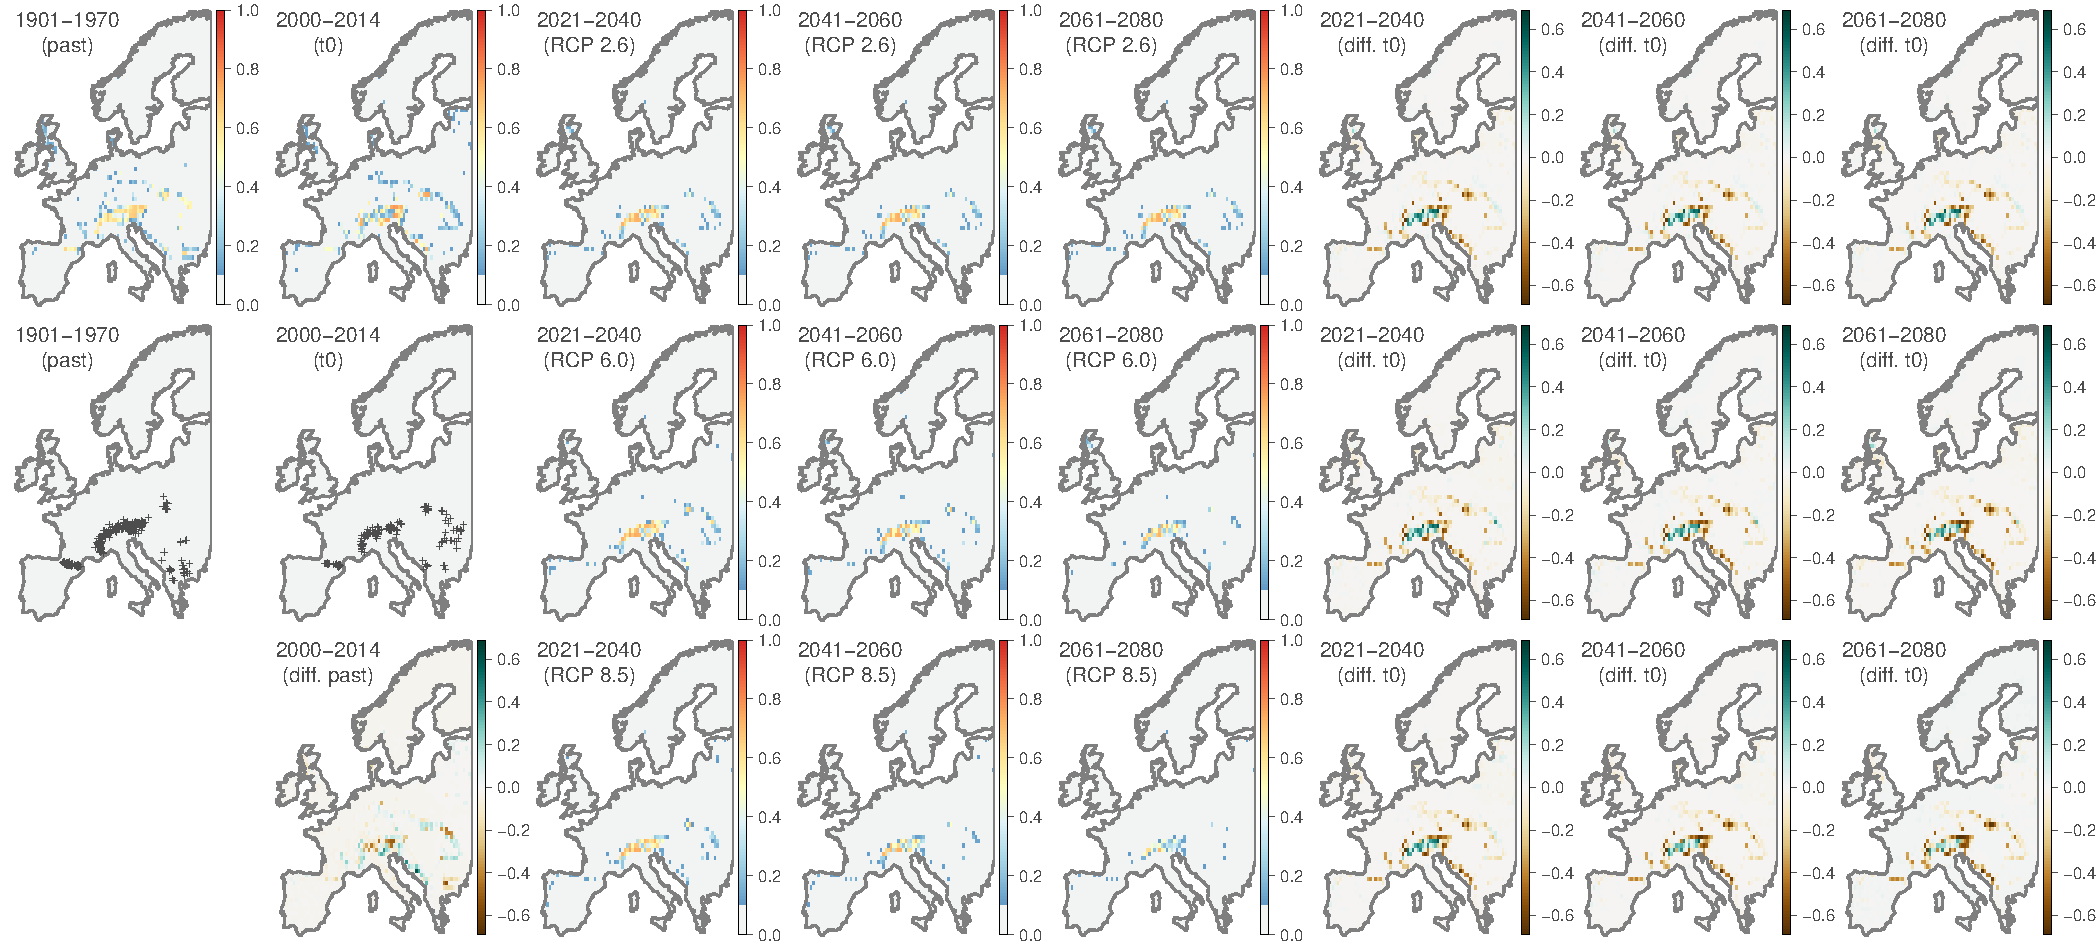
\includegraphics[width=1.00\textwidth]{All_the_species_projections/B_pyrenaeus_projections.pdf}}
\caption{\small{\textbf{Ecological niche modelling for \emph{Bombus pyrenaeus}.}
We report the projection for the current period as well as differences between future and current projections.}}
\label{FigureS42}
\end{figure}
\renewcommand{\thefigure}{S43}
\begin{figure}[H]
\centering
\makebox[\textwidth][c]{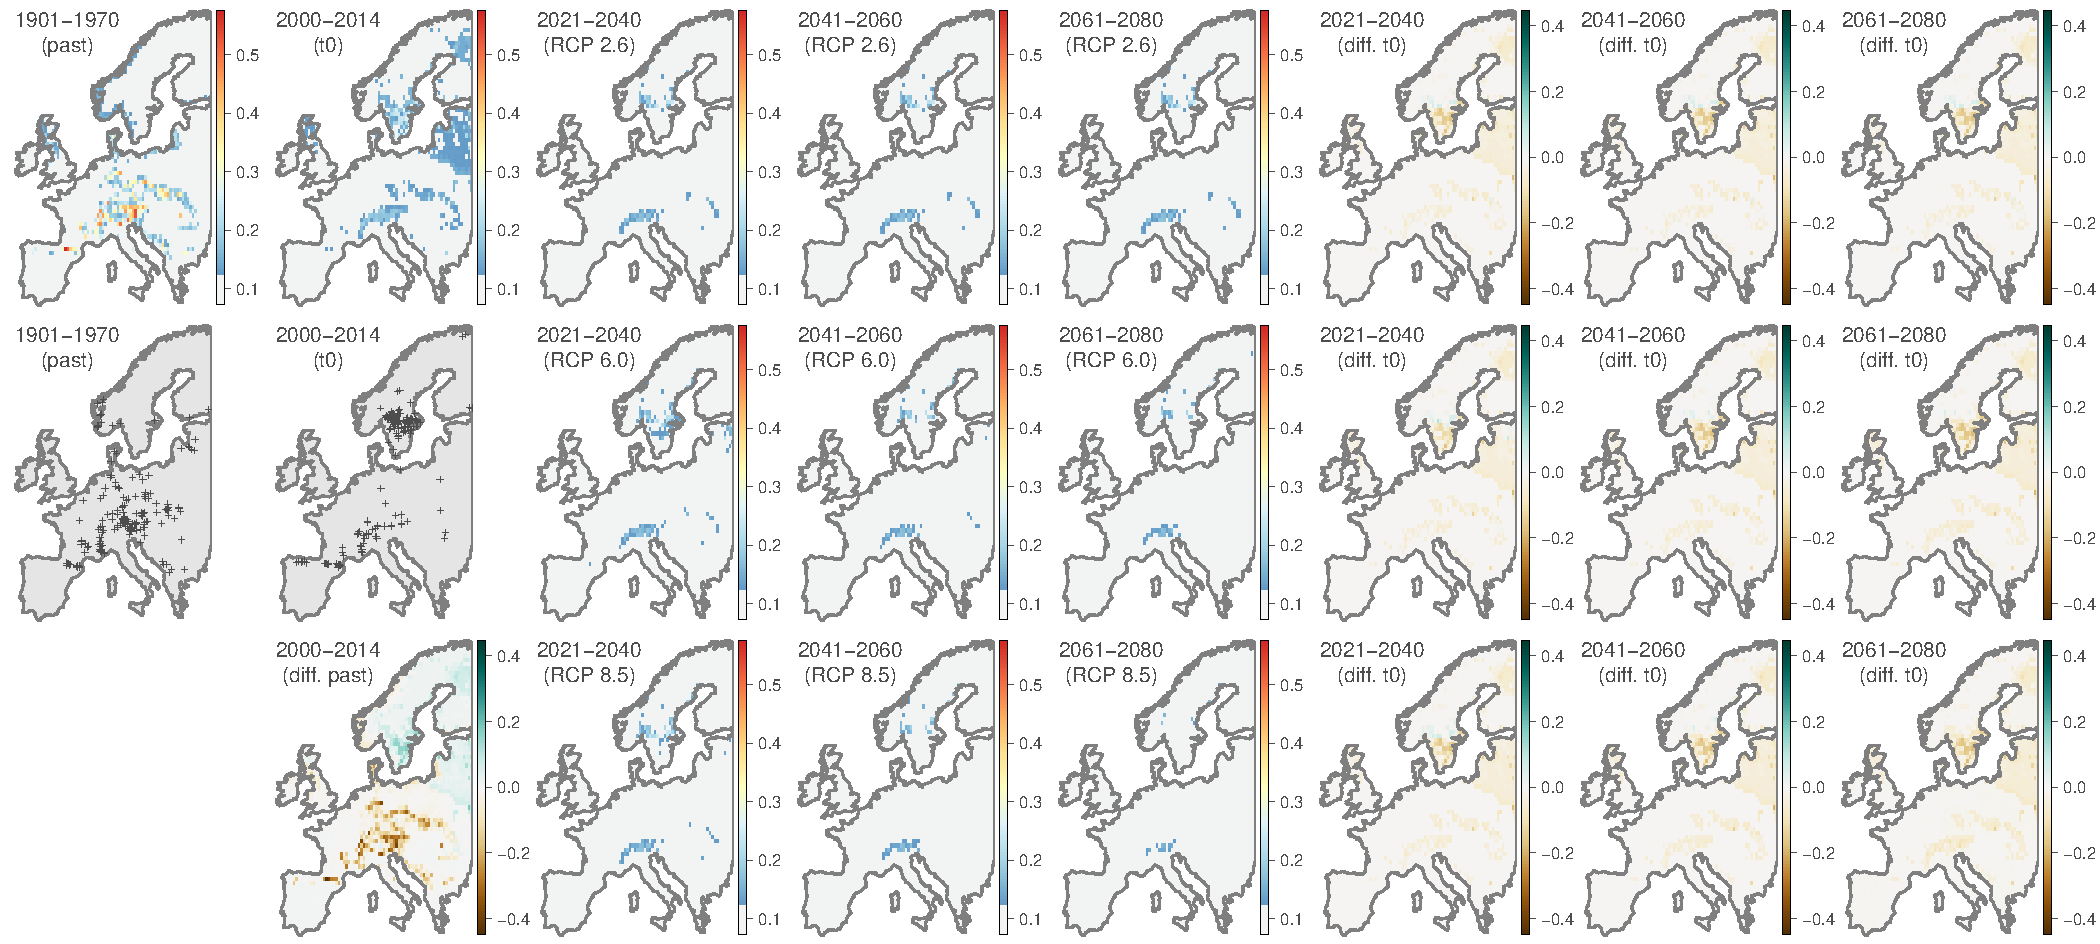
\includegraphics[width=1.00\textwidth]{All_the_species_projections/B_quadricolor_projections.pdf}}
\caption{\small{\textbf{Ecological niche modelling for \emph{Bombus quadricolor}.}
We report the projection for the current period as well as differences between future and current projections.}}
\label{FigureS43}
\end{figure}
\renewcommand{\thefigure}{S44}
\begin{figure}[H]
\centering
\makebox[\textwidth][c]{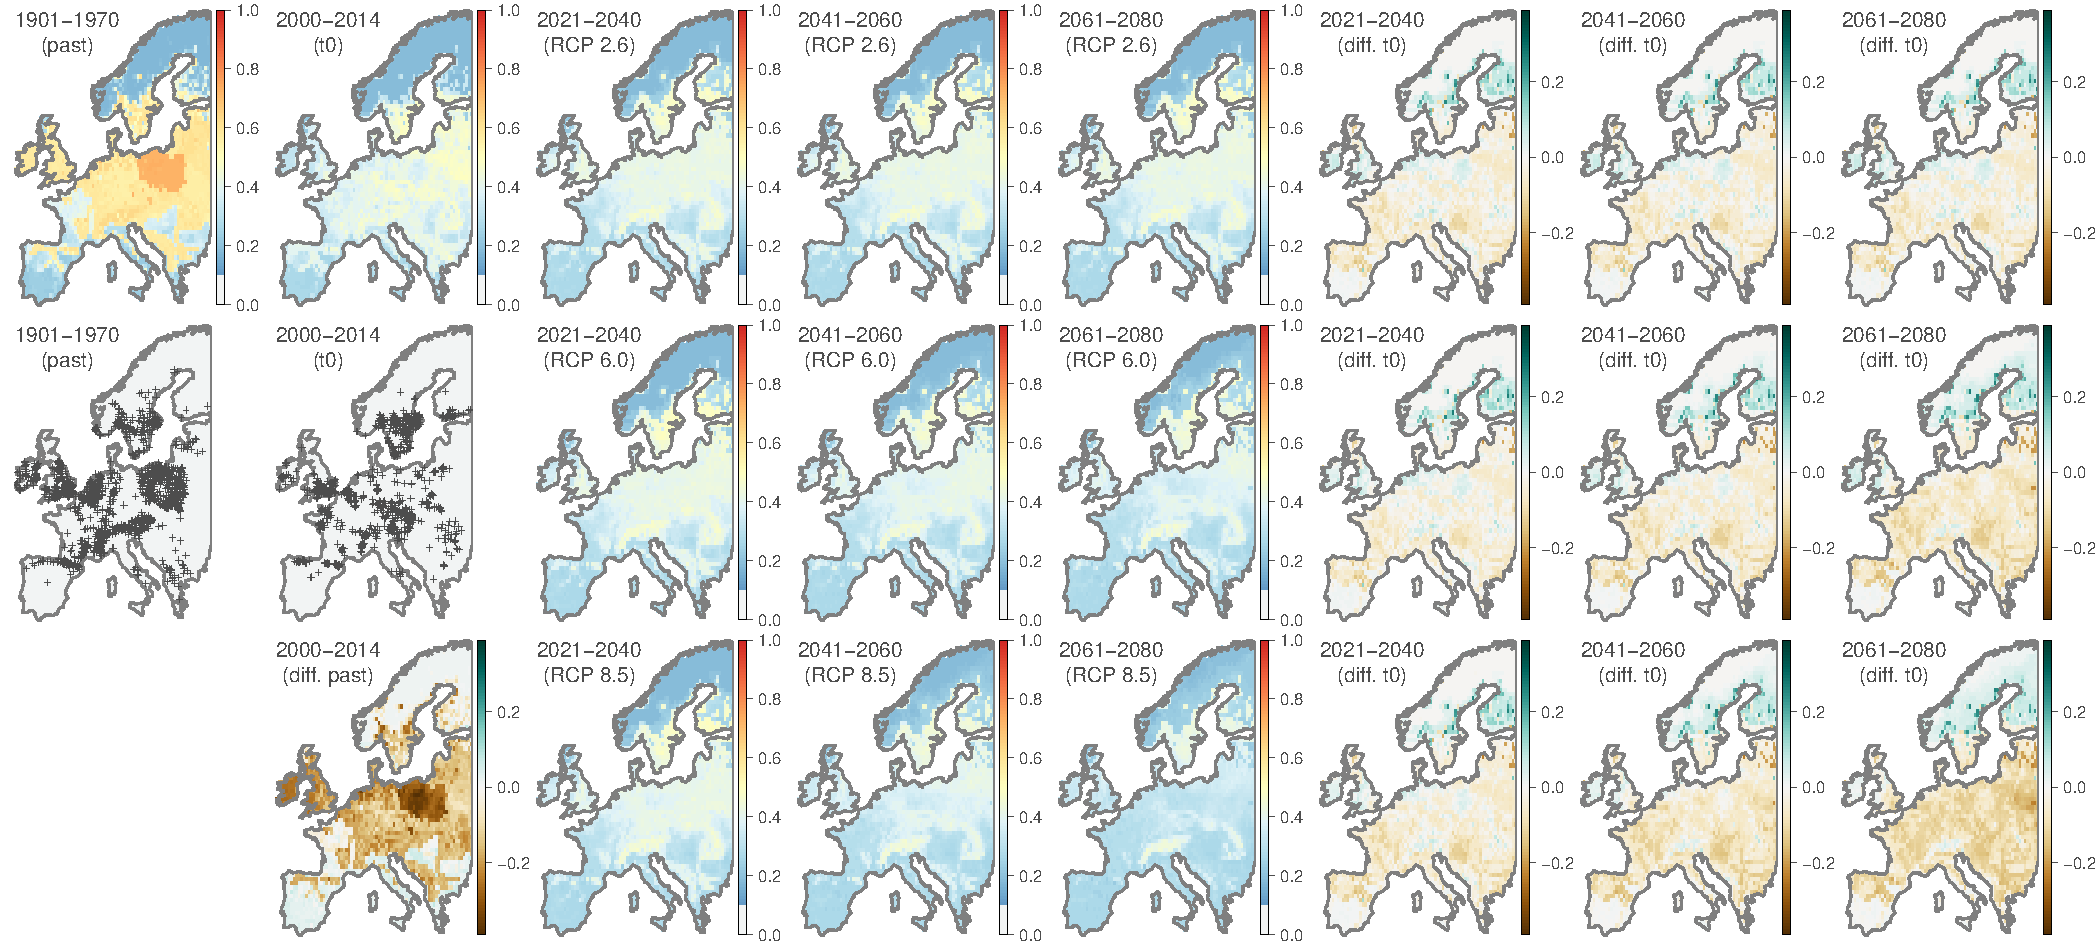
\includegraphics[width=1.00\textwidth]{All_the_species_projections/B_ruderarius_projections.pdf}}
\caption{\small{\textbf{Ecological niche modelling for \emph{Bombus ruderarius}.}
We report the projection for the current period as well as differences between future and current projections.}}
\label{FigureS44}
\end{figure}
\renewcommand{\thefigure}{S45}
\begin{figure}[H]
\centering
\makebox[\textwidth][c]{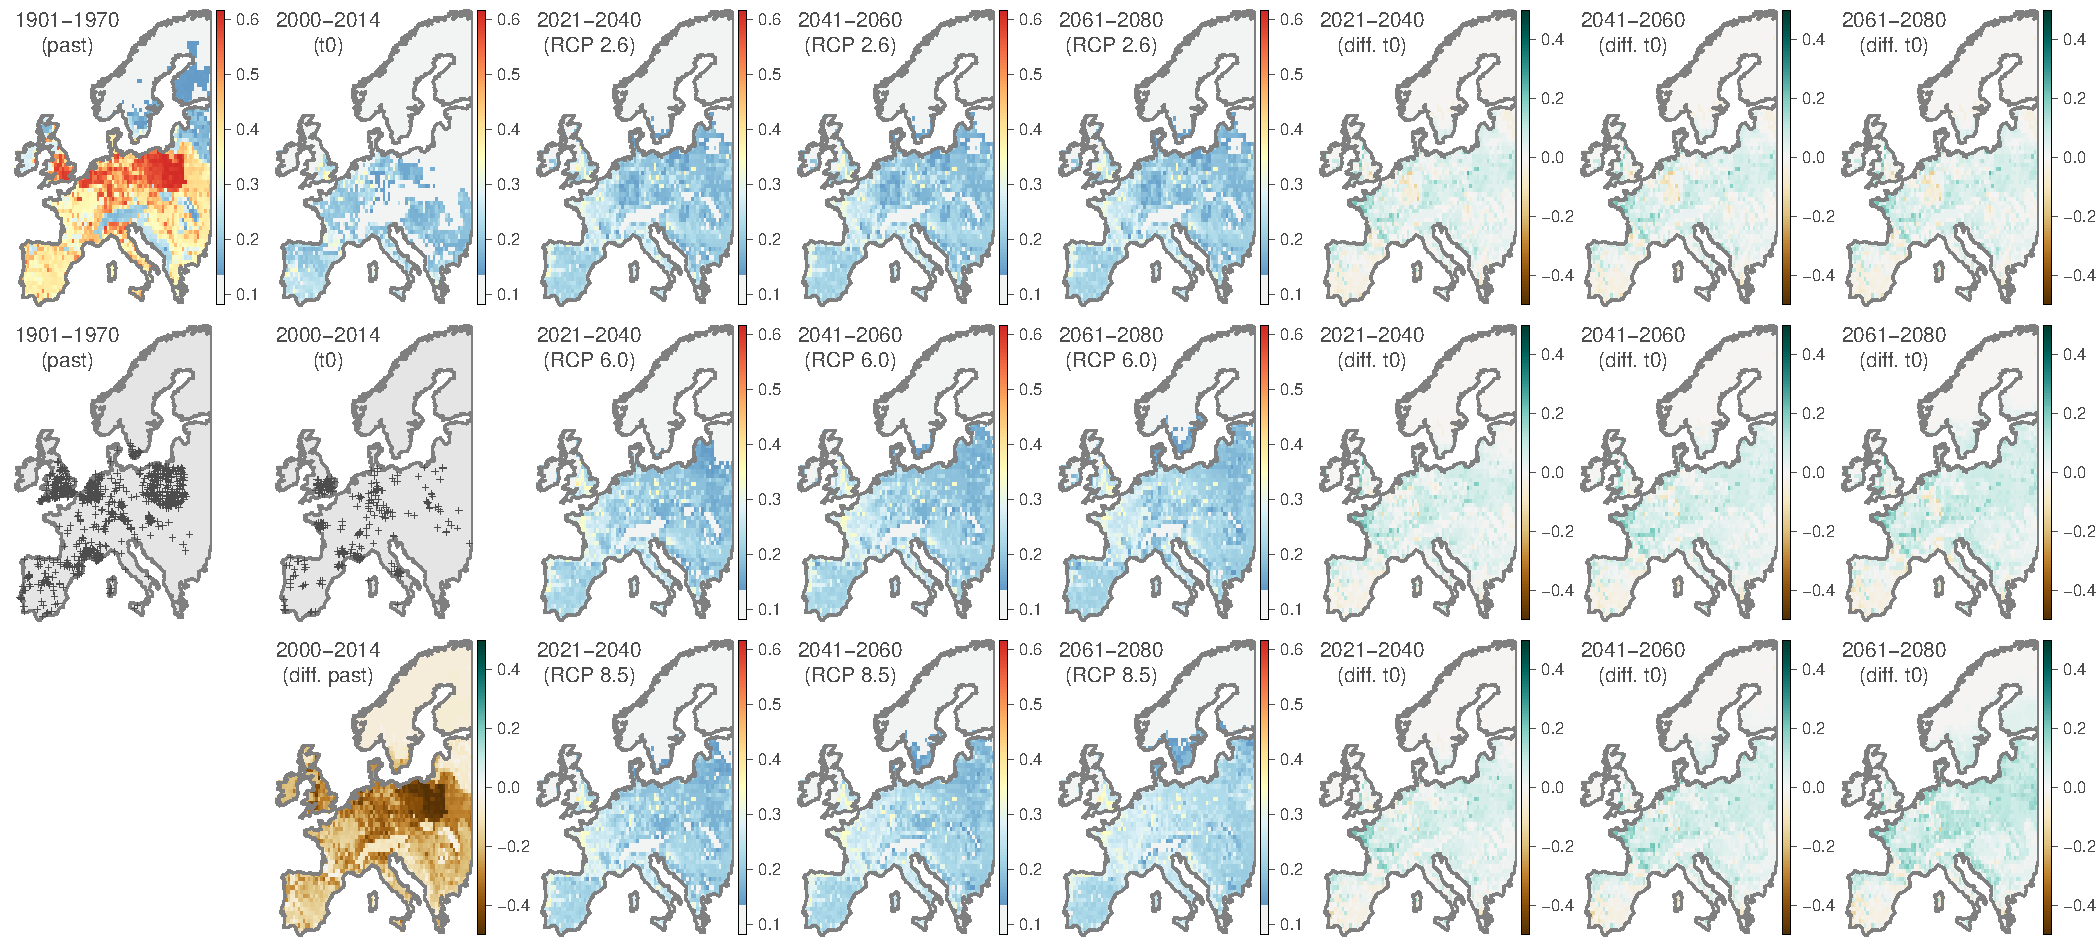
\includegraphics[width=1.00\textwidth]{All_the_species_projections/B_ruderatus_projections.pdf}}
\caption{\small{\textbf{Ecological niche modelling for \emph{Bombus ruderatus}.}
We report the projection for the current period as well as differences between future and current projections.}}
\label{FigureS45}
\end{figure}
\renewcommand{\thefigure}{S46}
\begin{figure}[H]
\centering
\makebox[\textwidth][c]{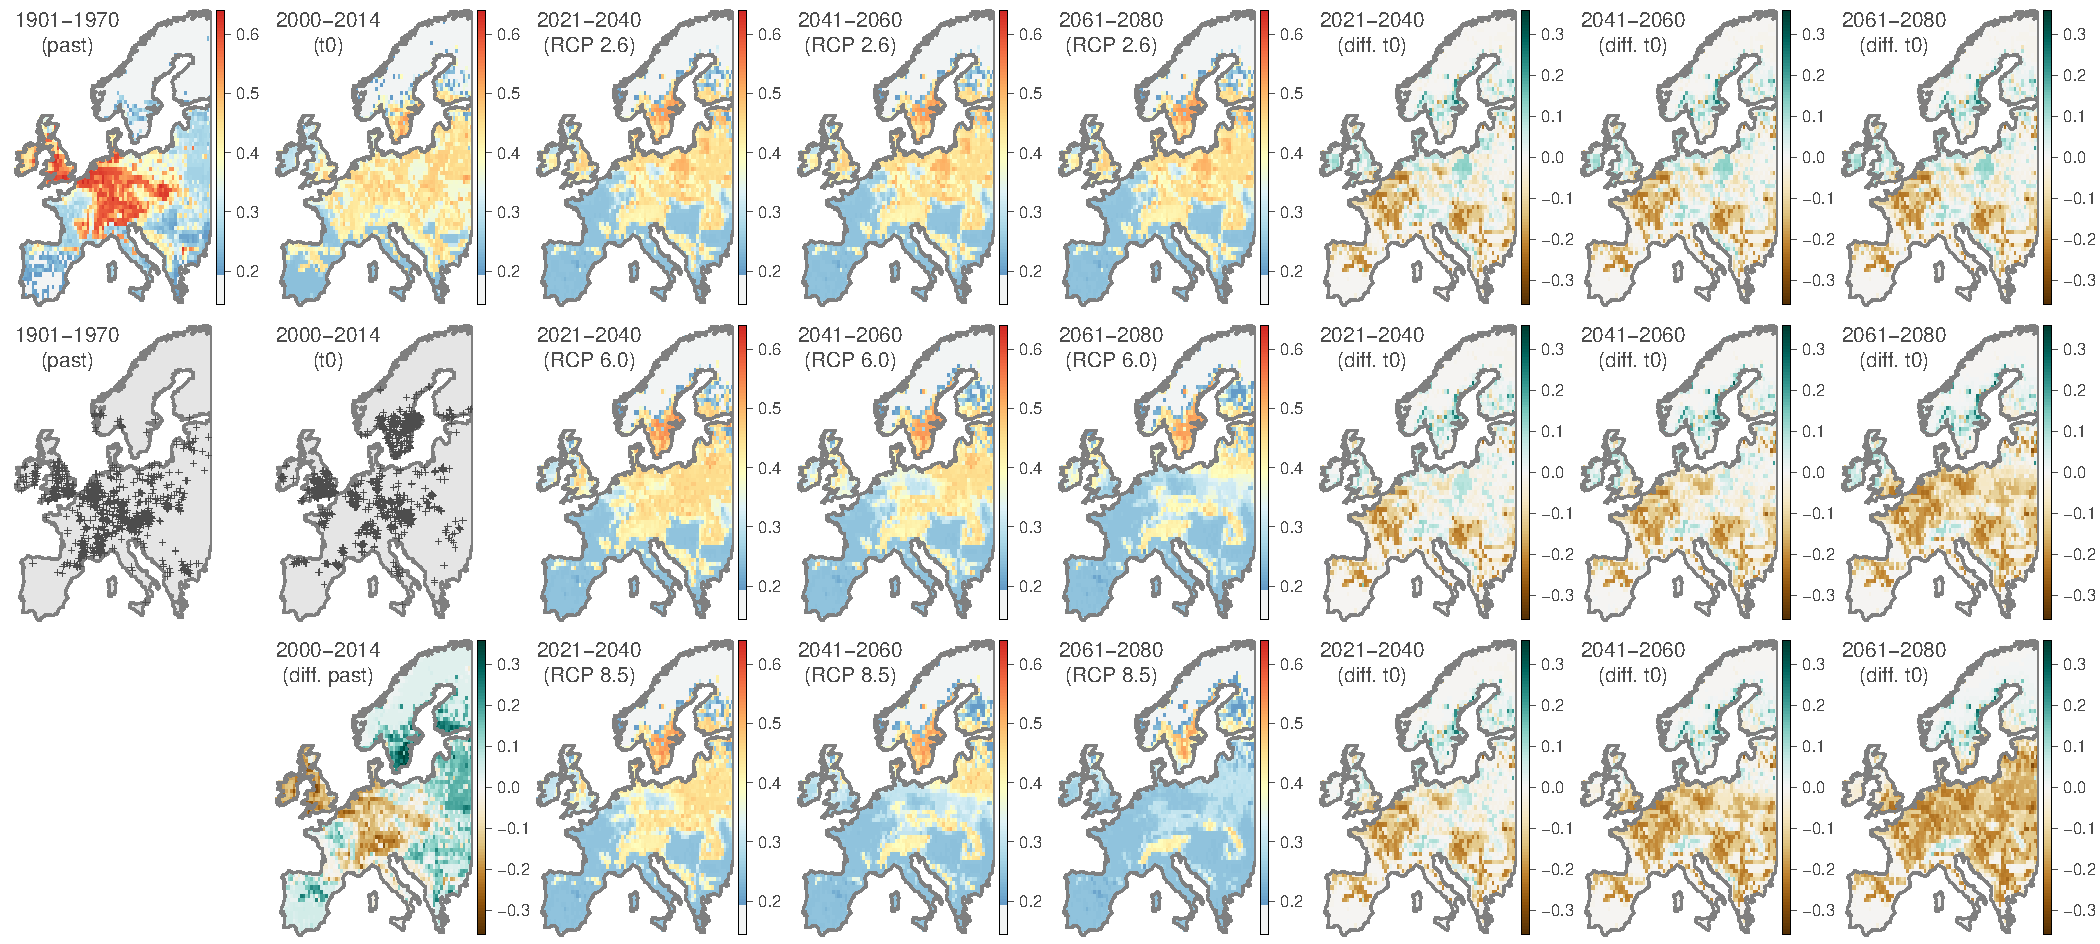
\includegraphics[width=1.00\textwidth]{All_the_species_projections/B_rupestris_projections.pdf}}
\caption{\small{\textbf{Ecological niche modelling for \emph{Bombus rupestris}.}
We report the projection for the current period as well as differences between future and current projections.}}
\label{FigureS46}
\end{figure}
\renewcommand{\thefigure}{S47}
\begin{figure}[H]
\centering
\makebox[\textwidth][c]{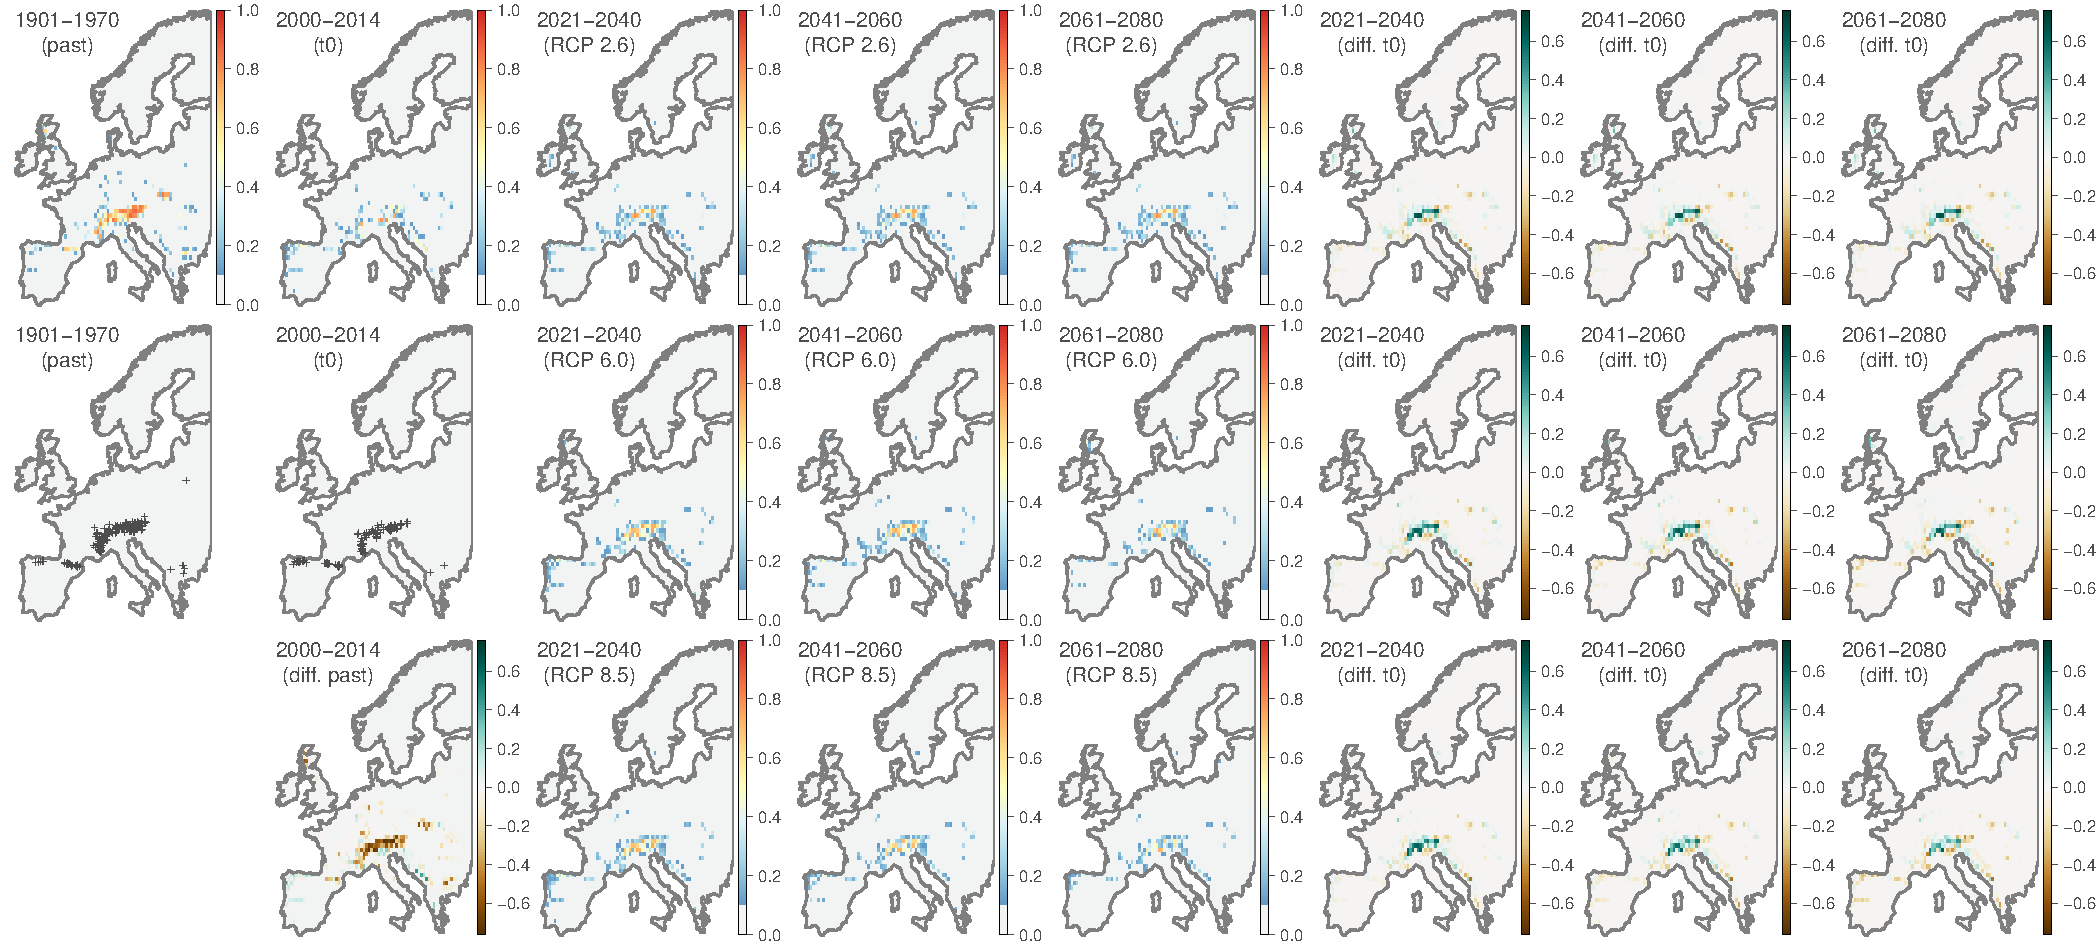
\includegraphics[width=1.00\textwidth]{All_the_species_projections/B_sichelii_projections.pdf}}
\caption{\small{\textbf{Ecological niche modelling for \emph{Bombus sichelii}.}
We report the projection for the current period as well as differences between future and current projections.}}
\label{FigureS47}
\end{figure}
\renewcommand{\thefigure}{S48}
\begin{figure}[H]
\centering
\makebox[\textwidth][c]{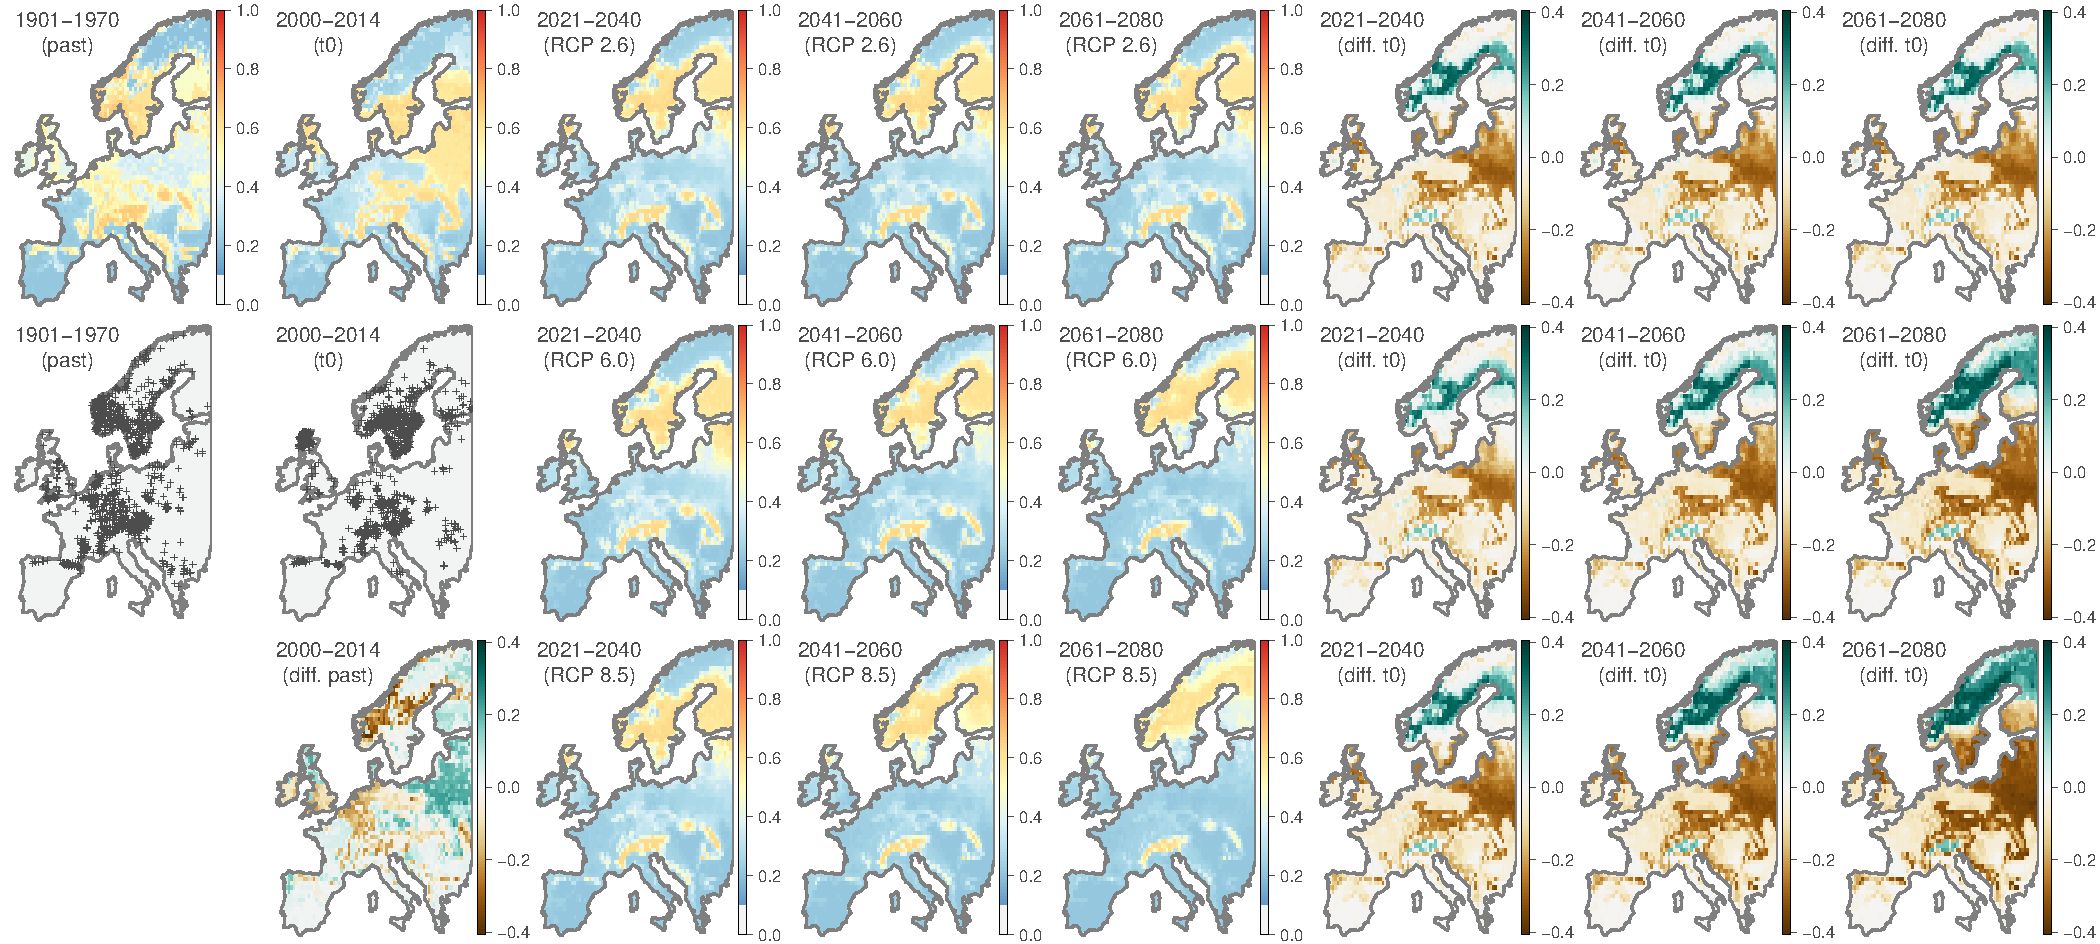
\includegraphics[width=1.00\textwidth]{All_the_species_projections/B_soroeensis_projections.pdf}}
\caption{\small{\textbf{Ecological niche modelling for \emph{Bombus soroeensis}.}
We report the projection for the current period as well as differences between future and current projections.}}
\label{FigureS48}
\end{figure}
\renewcommand{\thefigure}{S49}
\begin{figure}[H]
\centering
\makebox[\textwidth][c]{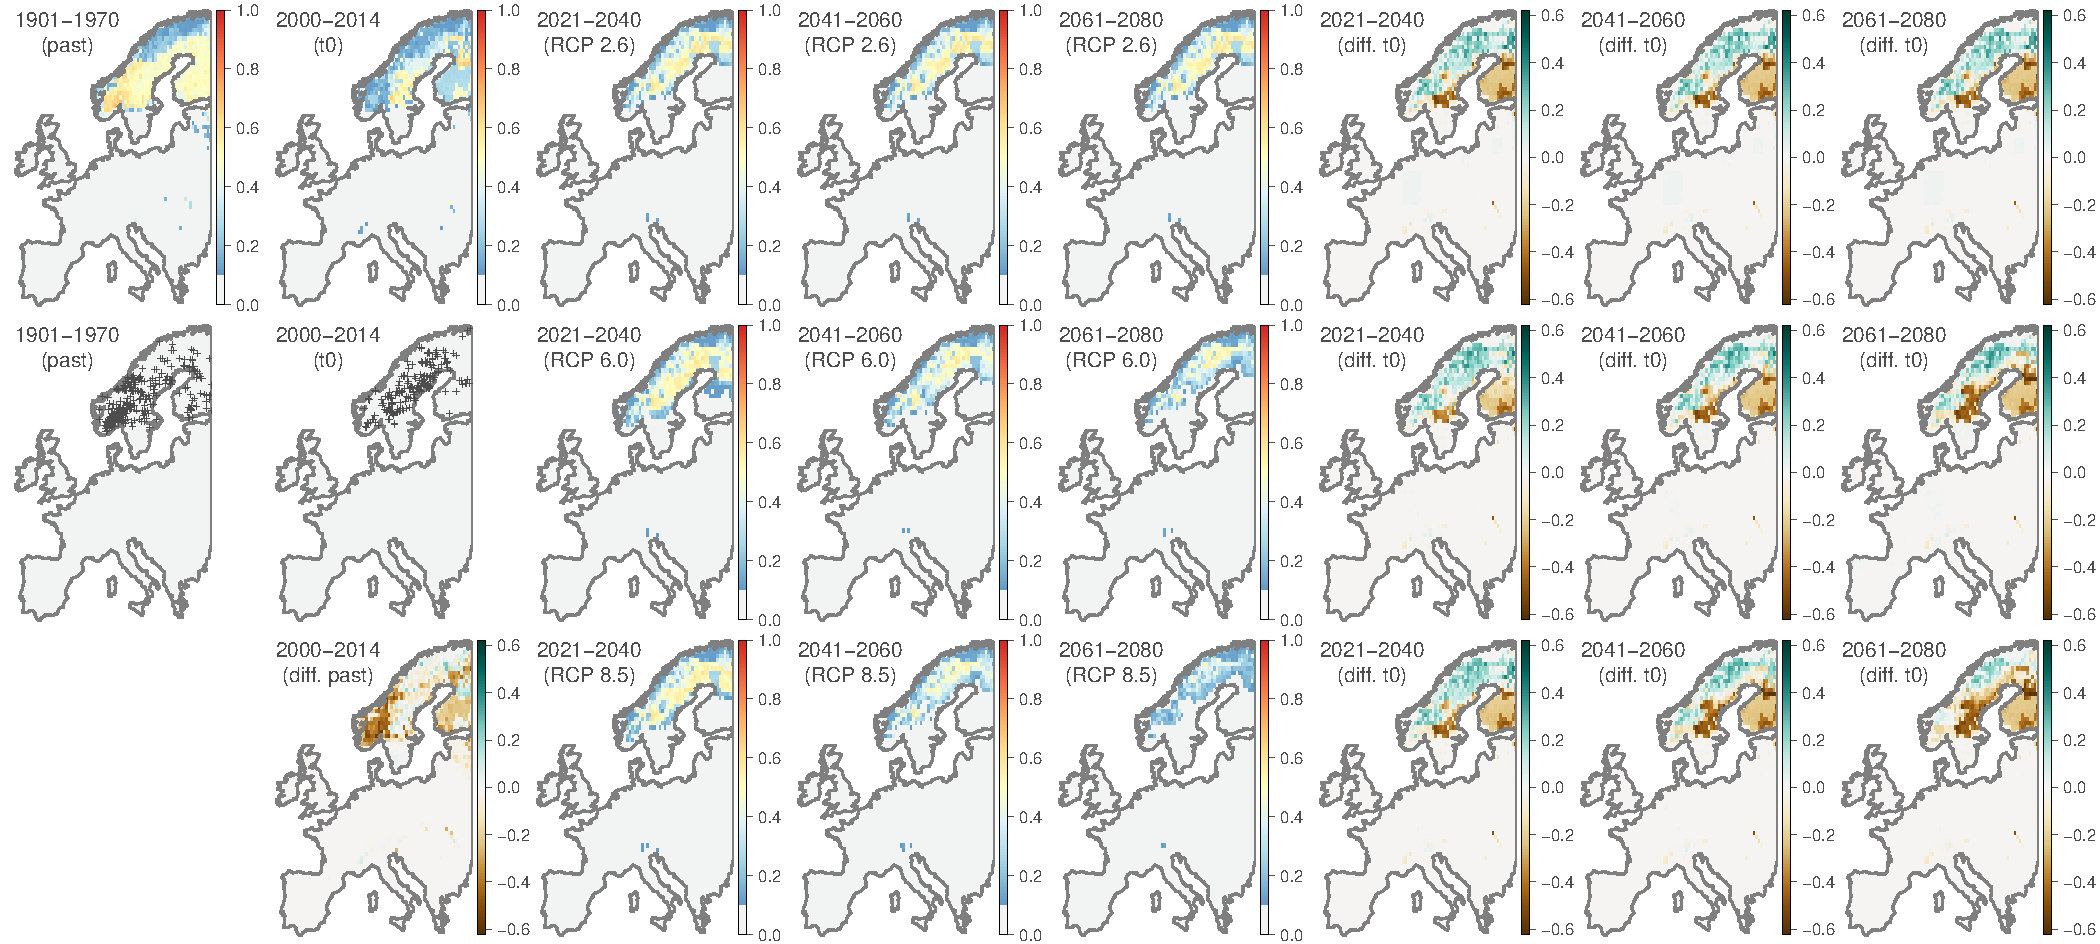
\includegraphics[width=1.00\textwidth]{All_the_species_projections/B_sporadicus_projections.pdf}}
\caption{\small{\textbf{Ecological niche modelling for \emph{Bombus sporadicus}.}
We report the projection for the current period as well as differences between future and current projections.}}
\label{FigureS49}
\end{figure}
\renewcommand{\thefigure}{S50}
\begin{figure}[H]
\centering
\makebox[\textwidth][c]{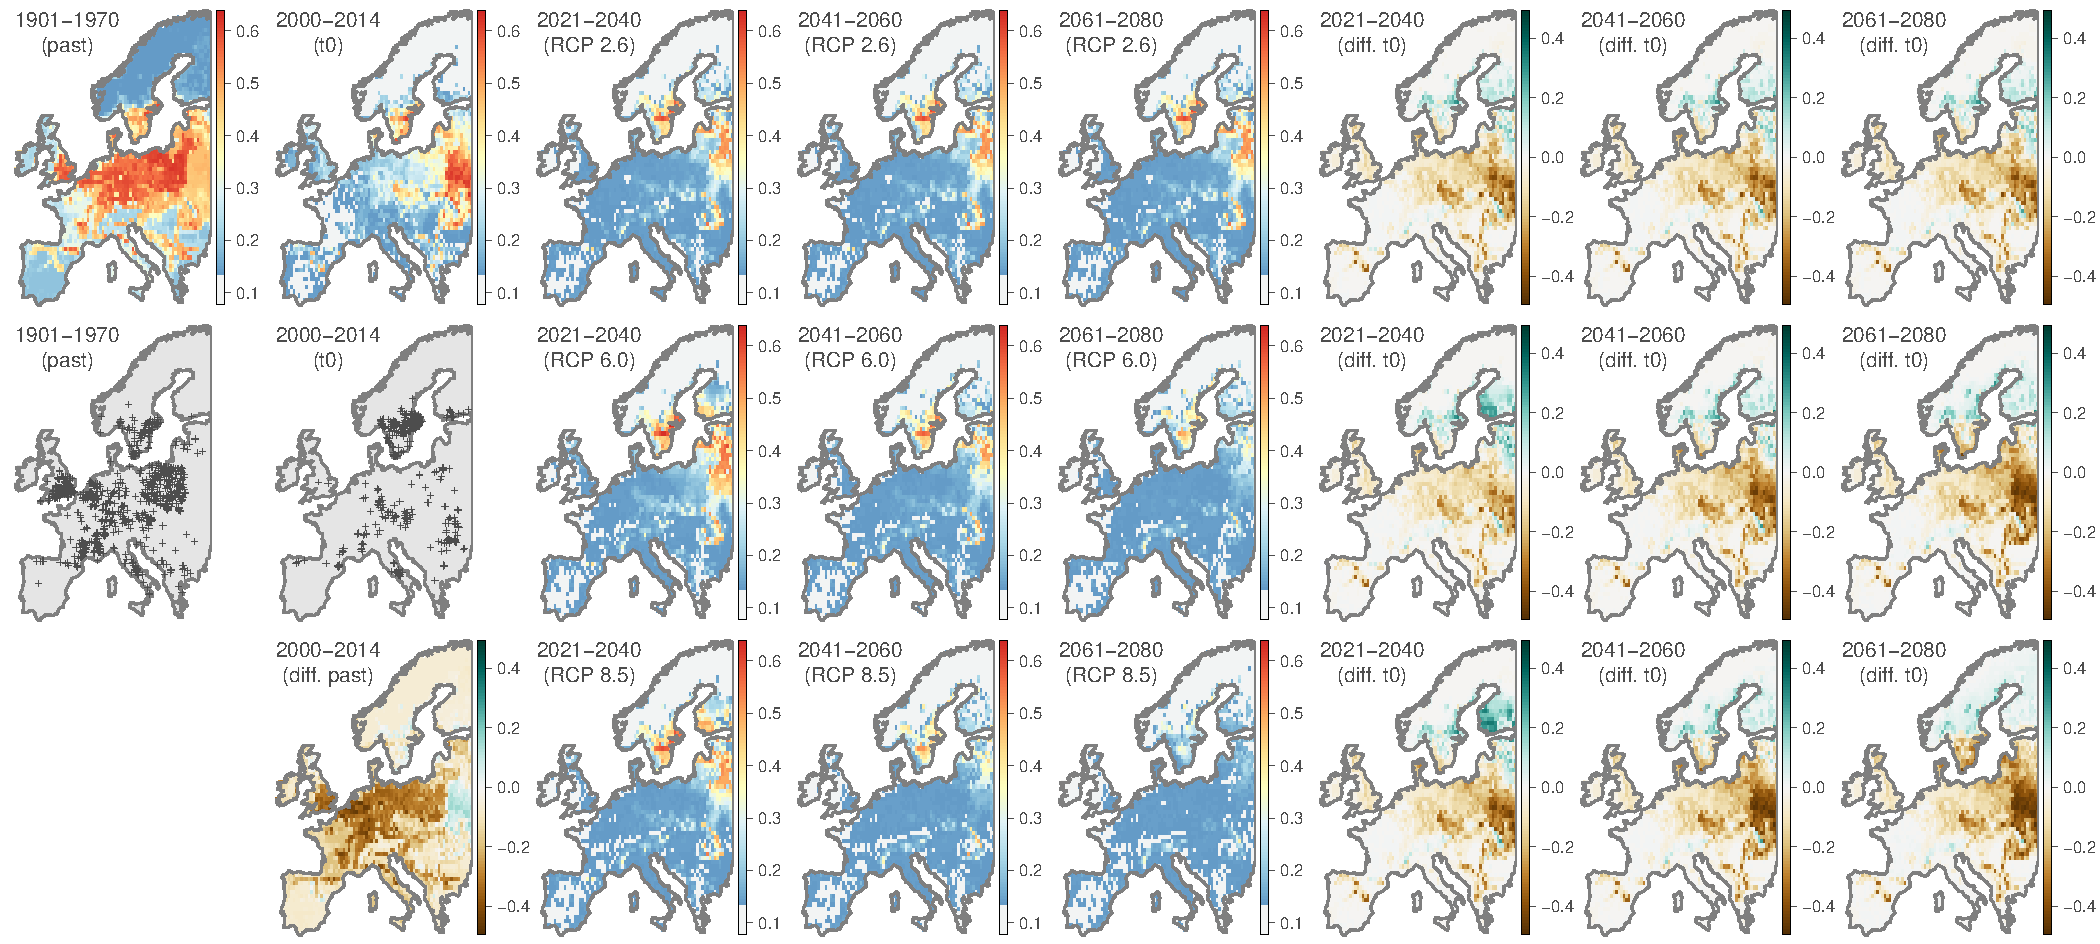
\includegraphics[width=1.00\textwidth]{All_the_species_projections/B_subterraneus_projections.pdf}}
\caption{\small{\textbf{Ecological niche modelling for \emph{Bombus subterraneus}.}
We report the projection for the current period as well as differences between future and current projections.}}
\label{FigureS50}
\end{figure}
\renewcommand{\thefigure}{S51}
\begin{figure}[H]
\centering
\makebox[\textwidth][c]{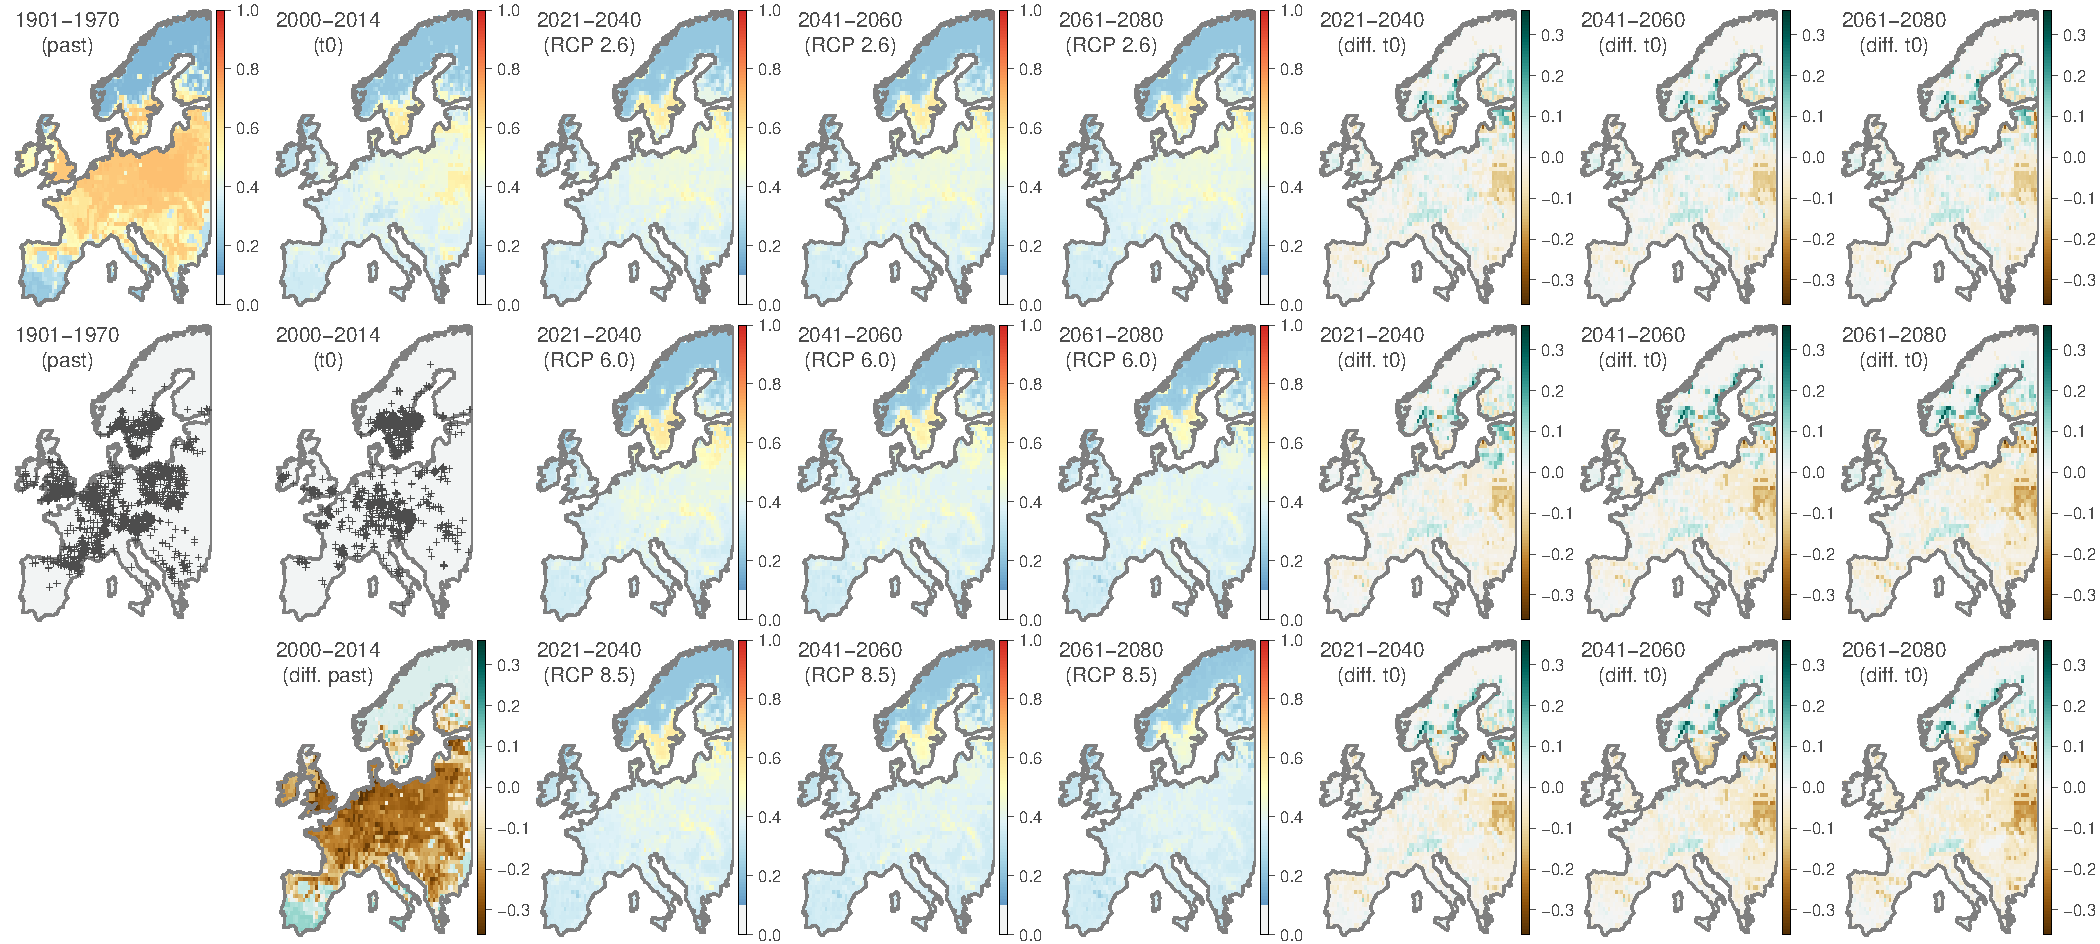
\includegraphics[width=1.00\textwidth]{All_the_species_projections/B_sylvarum_projections.pdf}}
\caption{\small{\textbf{Ecological niche modelling for \emph{Bombus sylvarum}.}
We report the projection for the current period as well as differences between future and current projections.}}
\label{FigureS51}
\end{figure}
\renewcommand{\thefigure}{S52}
\begin{figure}[H]
\centering
\makebox[\textwidth][c]{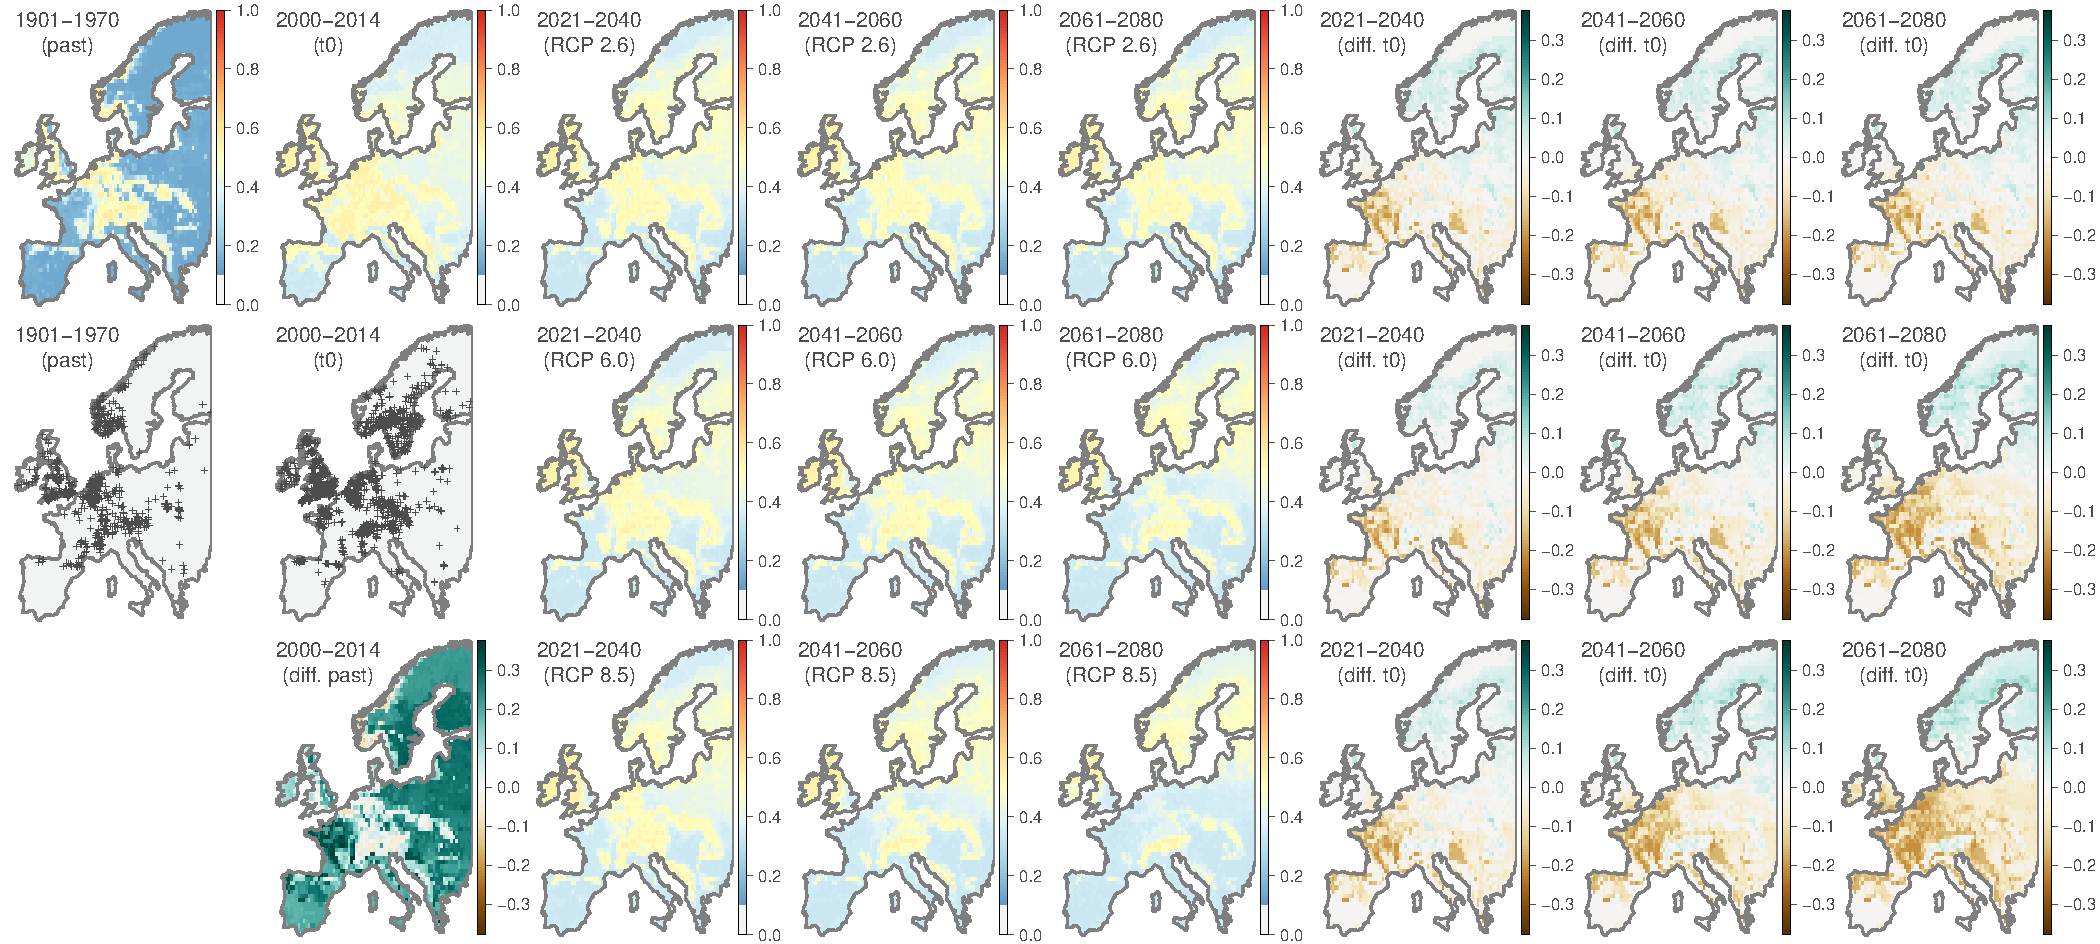
\includegraphics[width=1.00\textwidth]{All_the_species_projections/B_sylvestris_projections.pdf}}
\caption{\small{\textbf{Ecological niche modelling for \emph{Bombus sylvestris}.}
We report the projection for the current period as well as differences between future and current projections.}}
\label{FigureS52}
\end{figure}
\renewcommand{\thefigure}{S53}
\begin{figure}[H]
\centering
\makebox[\textwidth][c]{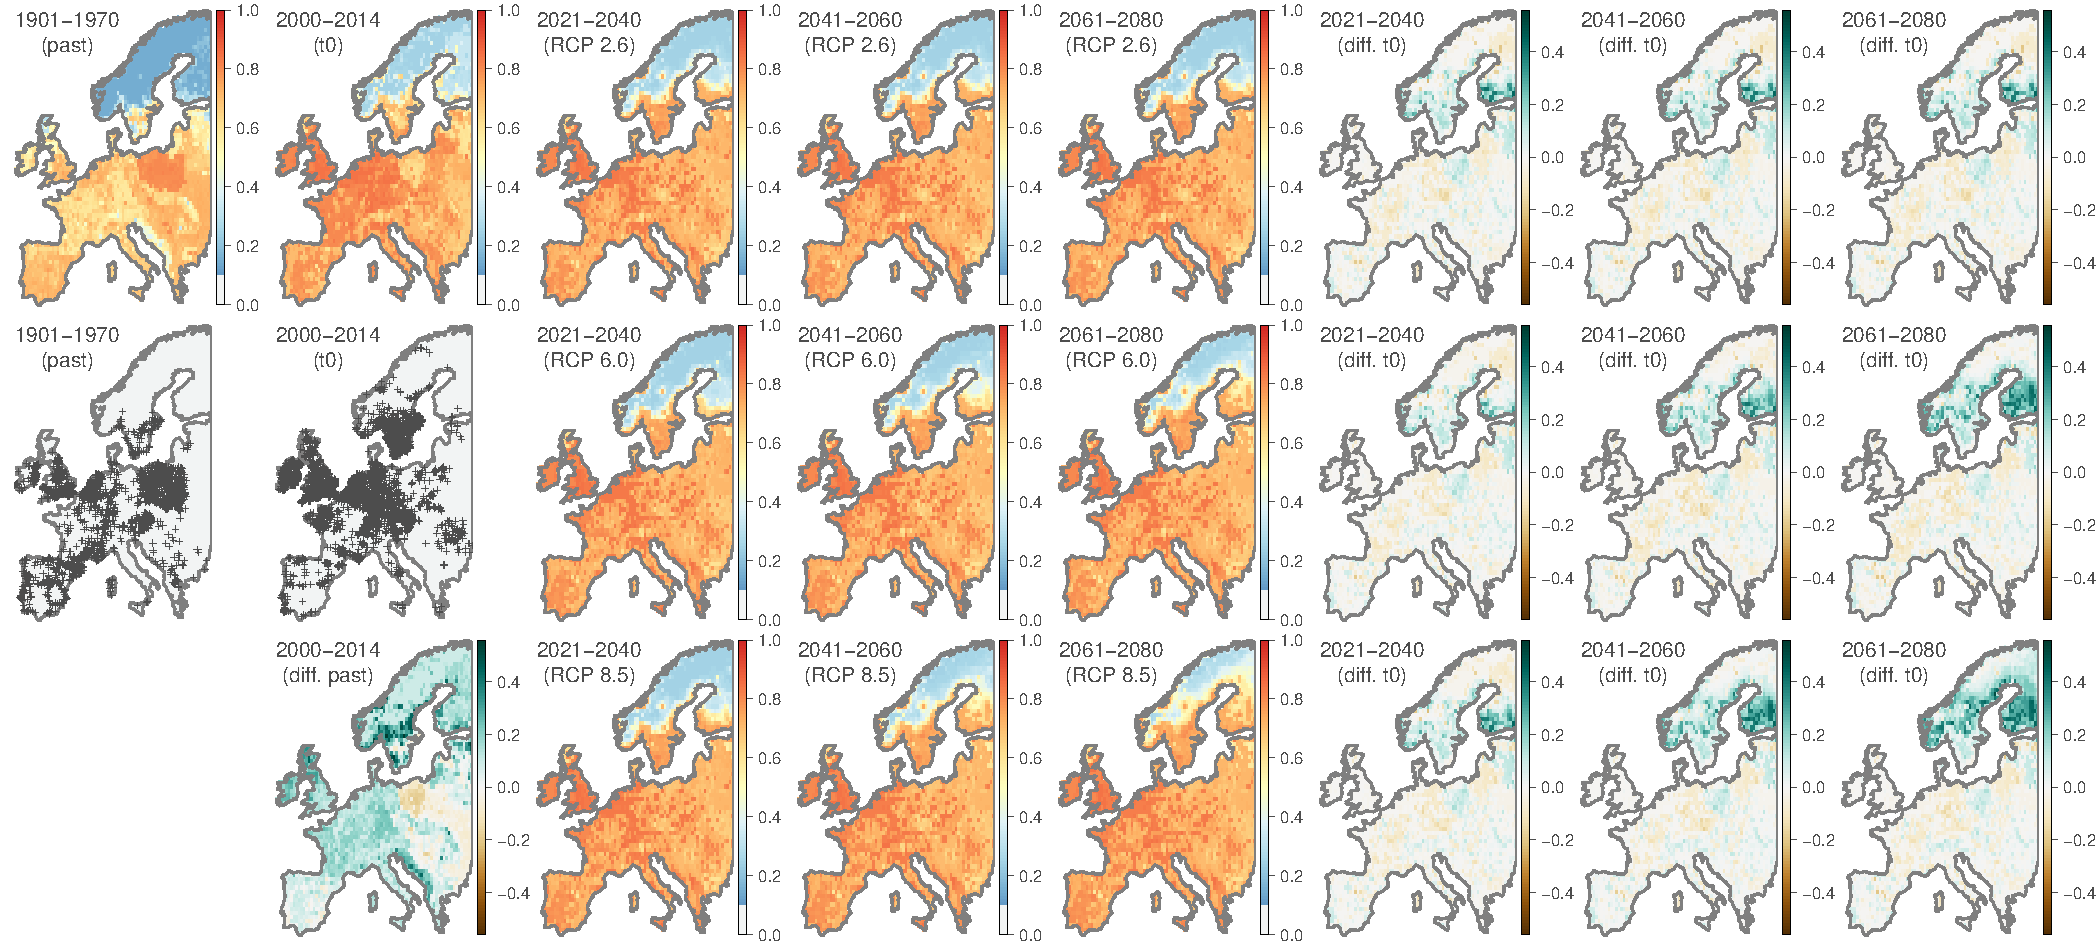
\includegraphics[width=1.00\textwidth]{All_the_species_projections/B_terrestris_projections.pdf}}
\caption{\small{\textbf{Ecological niche modelling for \emph{Bombus terrestris}.}
We report the projection for the current period as well as differences between future and current projections.}}
\label{FigureS53}
\end{figure}
\renewcommand{\thefigure}{S54}
\begin{figure}[H]
\centering
\makebox[\textwidth][c]{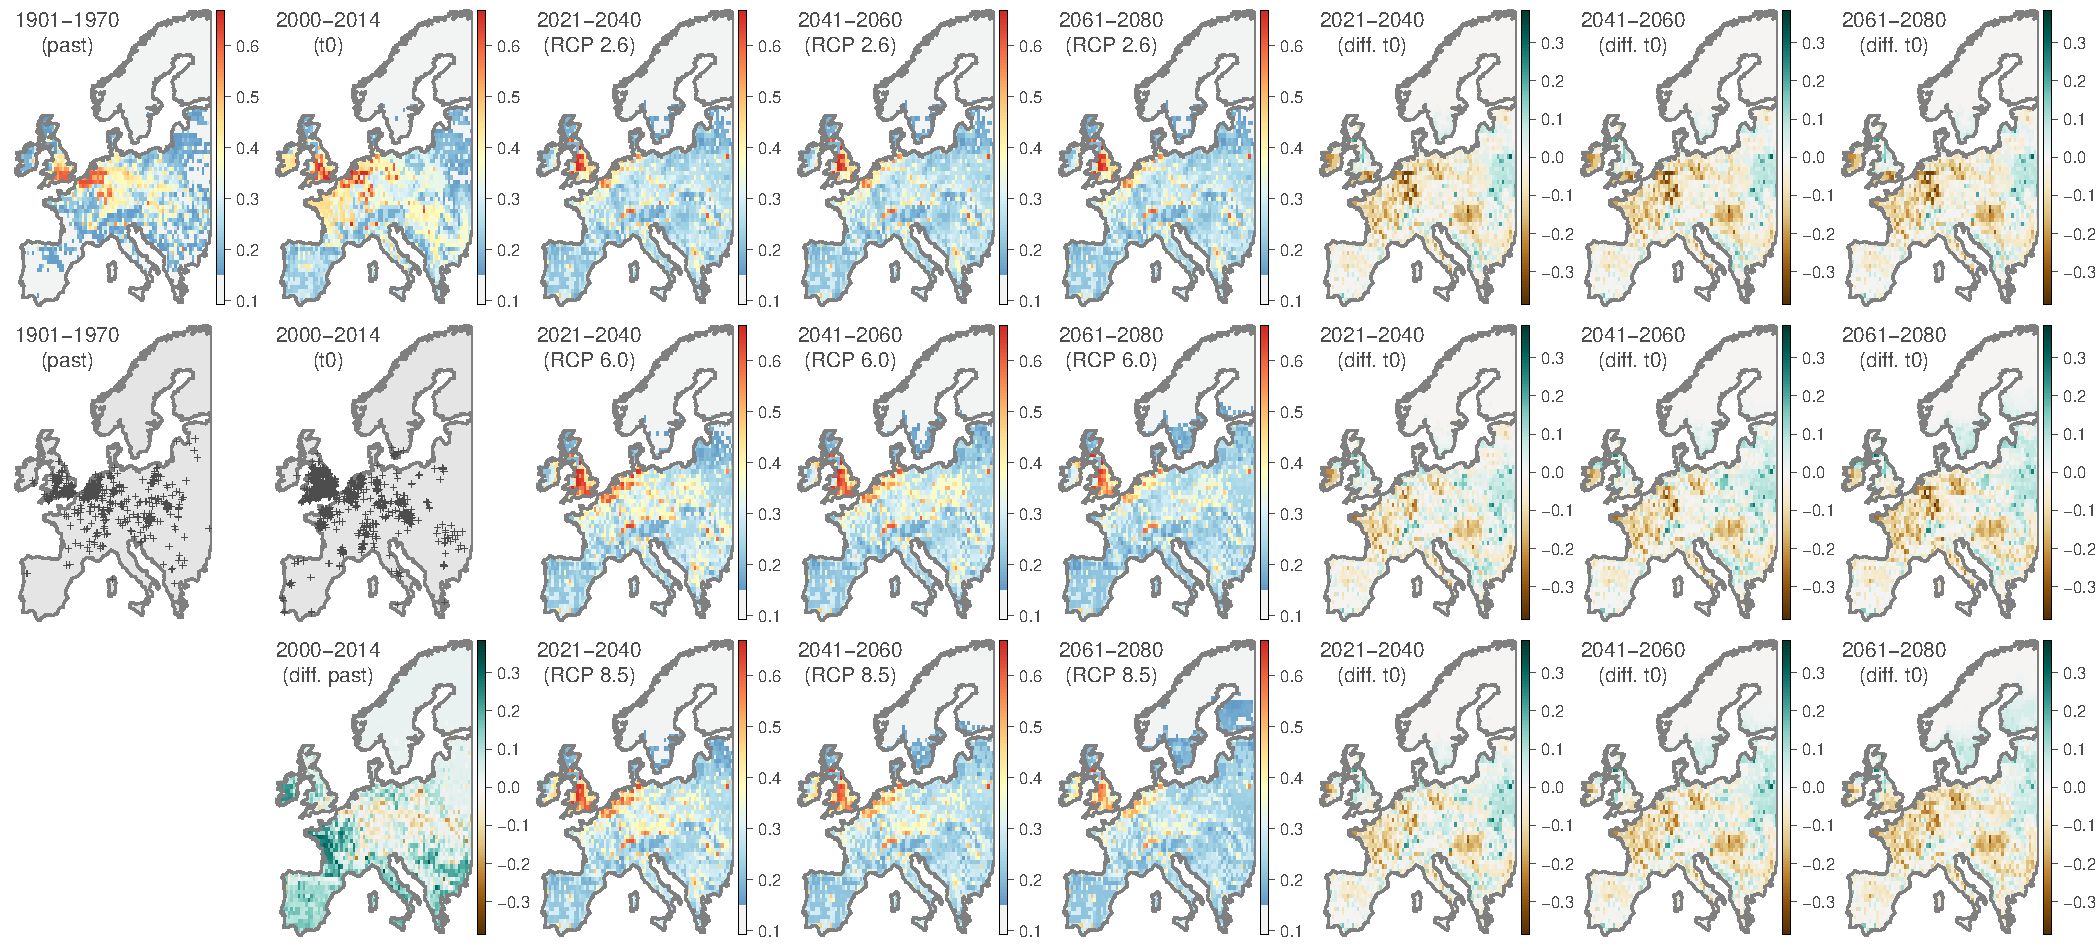
\includegraphics[width=1.00\textwidth]{All_the_species_projections/B_vestalis_projections.pdf}}
\caption{\small{\textbf{Ecological niche modelling for \emph{Bombus vestalis}.}
We report the projection for the current period as well as differences between future and current projections.}}
\label{FigureS54}
\end{figure}
\renewcommand{\thefigure}{S55}
\begin{figure}[H]
\centering
\makebox[\textwidth][c]{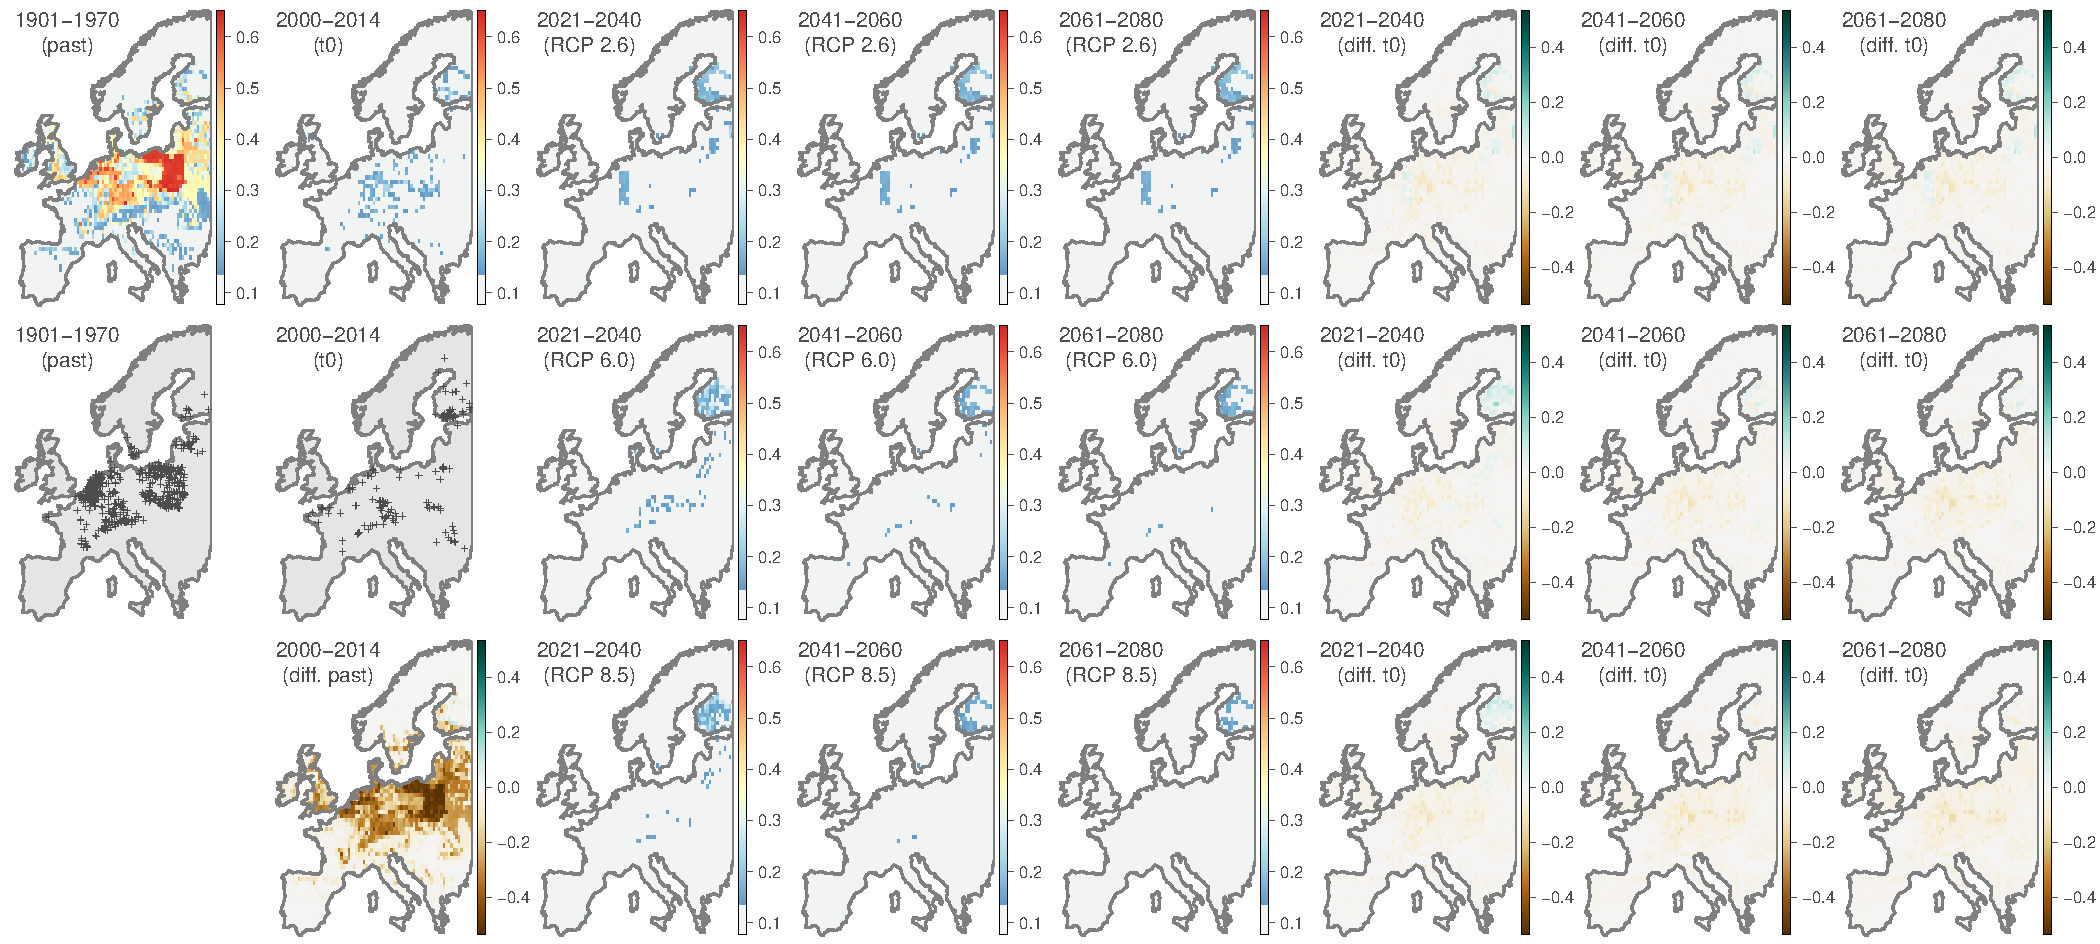
\includegraphics[width=1.00\textwidth]{All_the_species_projections/B_veteranus_projections.pdf}}
\caption{\small{\textbf{Ecological niche modelling for \emph{Bombus veteranus}.}
We report the projection for the current period as well as differences between future and current projections.}}
\label{FigureS55}
\end{figure}
\renewcommand{\thefigure}{S56}
\begin{figure}[H]
\centering
\makebox[\textwidth][c]{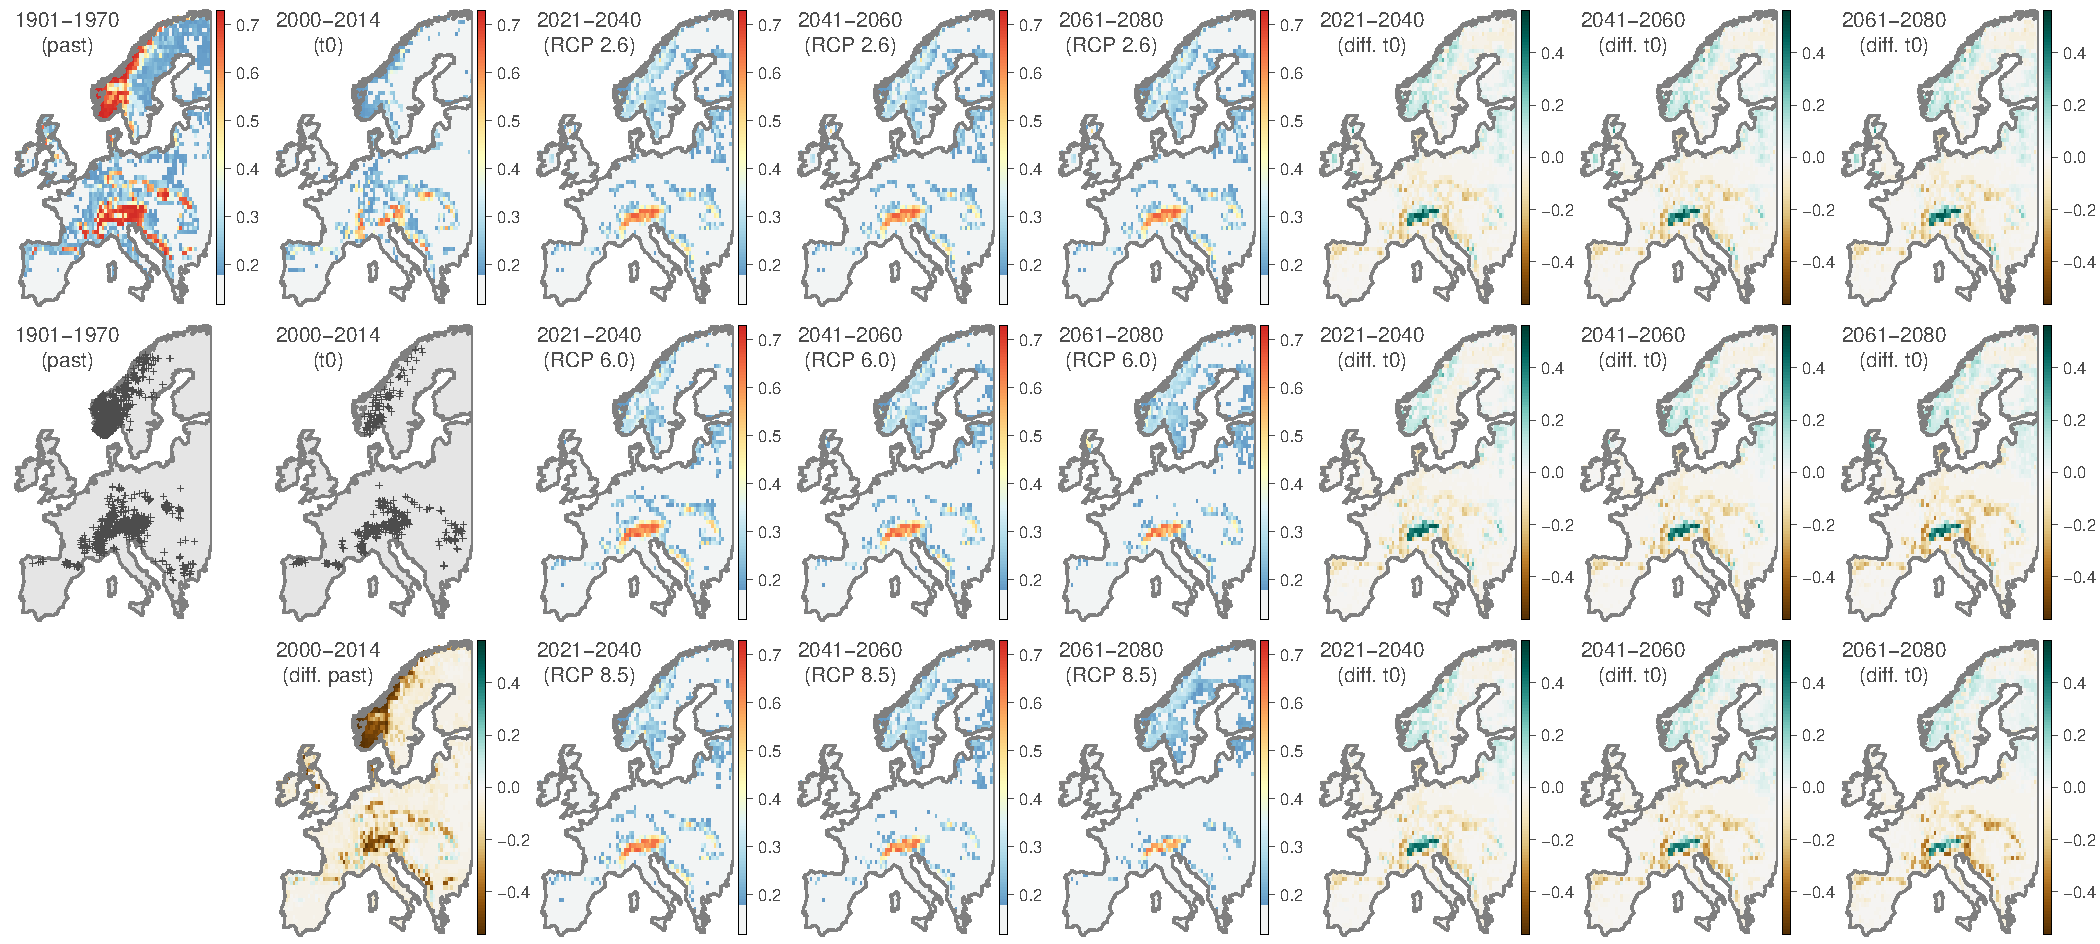
\includegraphics[width=1.00\textwidth]{All_the_species_projections/B_wurflenii_projections.pdf}}
\caption{\small{\textbf{Ecological niche modelling for \emph{Bombus wurflenii}.}
We report the projection for the current period as well as differences between future and current projections.}}
\label{FigureS56}
\end{figure}

\end{document}
